% Problems, Chapter 4: Multipoles, Electrostatics of Macroscopic Media, Dielectrics
% Jackson, Classical Electrodynamics, 3rd ed.
% Requires: amsmath, amssymb, tikz, booktabs (for the data tables)

\section*{Problems}

\Needspace{5\baselineskip}
\par\bigskip
\noindent\textbf{4.1}\quad Calculate the multipole moments $q_{lm}$ of the charge distributions shown as parts a and b. Try to obtain results for the nonvanishing moments valid for all $l$, but in each case find the first \emph{two} sets of nonvanishing moments at the very least.

\begin{center}
\begin{tikzpicture}[scale=1.5]
  % figure (a): +/-q at +/-a on x and y axes
  \draw (0,-1.5) -- (0,1.8) node[above] {$z$};
  \draw (-1.7,0) -- (1.7,0) node[right] {$y$};
  \draw (225:1.9) node[below left] {$x$} -- (45:1.9);
  \fill (0.85,0) circle (1.6pt) node[below right=0pt] {$q$};
  \fill (-0.85,0) circle (1.6pt) node[above left=0pt] {$-q$};
  \fill (45:0.85) circle (1.6pt) node[above left=0pt] {$-q$};
  \fill (225:0.85) circle (1.6pt) node[below left=0pt] {$q$};
  \node at (0.55,0.18) {$a$};
  \node at (-0.5,0.22) {$a$};
  \node at (48:0.42) {$a$};
  \node at (228:0.42) {$a$};
  \node at (0,-1.9) {(a)};
\end{tikzpicture}\hspace{3em}
\begin{tikzpicture}[scale=1.5]
  % figure (b): +q, -2q, +q on z axis
  \draw (0,-1.5) -- (0,1.8) node[above] {$z$};
  \draw (-1.7,0) -- (1.7,0) node[right] {$y$};
  \draw (225:1.9) node[below left] {$x$} -- (45:1.9);
  \fill (0,0.85) circle (1.6pt) node[left=3pt] {$+q$};
  \fill (0,0) circle (1.6pt) node[left=3pt] {$-2q$};
  \fill (0,-0.85) circle (1.6pt) node[left=3pt] {$+q$};
  \node[right] at (0.08,0.42) {$a$};
  \node[right] at (0.08,-0.42) {$a$};
  \node at (0,-1.9) {(b)};
\end{tikzpicture}
\par\vspace{0.5em}\textbf{Problem 4.1}
\end{center}

\begin{enumerate}
\item[(c)] For the charge distribution of the second set b write down the multipole expansion for the potential. Keeping only the lowest-order term in the expansion, plot the potential in the $x$-$y$ plane as a function of distance from the origin for distances greater than $a$.
\item[(d)] Calculate directly from Coulomb's law the exact potential for b in the $x$-$y$ plane. Plot it as a function of distance and compare with the result found in part c.
\end{enumerate}
Divide out the asymptotic form in parts c and d to see the behavior at large distances more clearly.
\solution

We use Jackson's (4.1), (4.3), and (4.7):
\[
q_{lm}=\int r^lY_{lm}^{*}\rho\,d^3r,\qquad
\Phi=\frac{1}{4\pi\epsilon_0}\sum_{l,m}\frac{4\pi}{2l+1}
\frac{q_{lm}Y_{lm}}{r^{l+1}},\qquad q_{l,-m}=(-1)^m q_{lm}^{*}.
\]
Here $Y_{lm}=N_{lm}P_l^m(\cos\theta)e^{im\phi}$ for $m\geq0$,
$N_{lm}=[(2l+1)(l-m)!/(4\pi(l+m)!)]^{1/2}$, and $P_l^m$
includes the Condon--Shortley factor $(-1)^m$.

\textbf{(a)} The positive $x$ axis points down and left in the drawing.
The charges are therefore $+q$ at $a\hat{\mathbf x},a\hat{\mathbf y}$ and
$-q$ at $-a\hat{\mathbf x},-a\hat{\mathbf y}$. Substitution gives
\begin{align*}
q_{lm}&=qa^lN_{lm}P_l^m(0)
[1+e^{-im\pi/2}-e^{-im\pi}-e^{-3im\pi/2}]\\
&=qa^lN_{lm}P_l^m(0)[1-(-1)^m][1+e^{-im\pi/2}].
\end{align*}
Even $l$ vanish by odd inversion symmetry; $P_l^m(0)=0$ when $l+m$
is odd. To evaluate the nonzero values, use Rodrigues' polynomial
and $P_l^m(x)=(-1)^m(1-x^2)^{m/2}d^mP_l/dx^m$:
\[
P_l(x)=2^{-l}\sum_{j=0}^{\lfloor l/2\rfloor}
\frac{(-1)^j(2l-2j)!}{j!(l-j)!(l-2j)!}\,x^{l-2j}.
\]
At $x=0$, only the term with $l-2j=m$ survives the $m$ derivatives.
For even $l+m$ this gives
\[
P_l^m(0)=(-1)^{(l+m)/2}
\frac{(l+m)!}{2^l[(l-m)/2]![(l+m)/2]!}
=(-1)^{(l+m)/2}\frac{(l+m-1)!!}{(l-m)!!}.
\]
The factor $1-(-1)^m$ in the charge sum also requires odd $m$.
For odd $l$ and positive odd $m\leq l$ the complete answer is
\[
\boxed{q_{lm}=2qa^lN_{lm}(-1)^{(l+m)/2}
\frac{(l+m-1)!!}{(l-m)!!}(1+e^{-im\pi/2}).}
\]
Negative $m$ follow by conjugation, and all remaining moments vanish.
The first two nonzero sets are
\[
q_{11}=-qa\sqrt{\frac{3}{2\pi}}(1-i),\qquad q_{1,-1}=-q_{11}^{*},
\]
\[
q_{31}=qa^3\sqrt{\frac{21}{16\pi}}(1-i),\quad
q_{33}=-qa^3\sqrt{\frac{35}{16\pi}}(1+i),\quad
q_{3,-1}=-q_{31}^{*},\quad q_{3,-3}=-q_{33}^{*}.
\]
As a check, $\mathbf p=2qa(\hat{\mathbf x}+\hat{\mathbf y})$ reproduces
$q_{11}$ through Jackson's (4.5).

\textbf{(b)} Axial symmetry permits only $m=0$. The central charge
contributes only to $l=0$, cancelling the other two charges. Since
$Y_{l0}(0)=\sqrt{(2l+1)/(4\pi)}$ and
$Y_{l0}(\pi)=(-1)^lY_{l0}(0)$,
\[
\boxed{q_{2n,0}=2qa^{2n}\sqrt{\frac{4n+1}{4\pi}},\quad n\geq1.}
\]
Thus $q_{20}=qa^2\sqrt{5/\pi}$ and $q_{40}=3qa^4/\sqrt\pi$ are the
first two sets; all other moments vanish.

\textbf{(c)} Substitution into the potential, using
$Y_{l0}=\sqrt{(2l+1)/(4\pi)}P_l$, gives
\[
\boxed{\Phi(r,\theta)=\frac{2q}{4\pi\epsilon_0r}
\sum_{n=1}^{\infty}\left(\frac ar\right)^{2n}P_{2n}(\cos\theta),\quad r>a.}
\]
In the $x$--$y$ plane let $s=\sqrt{x^2+y^2}$. As $P_2(0)=-1/2$,
$\Phi_2(s)=-qa^2/(4\pi\epsilon_0s^3)$.

\textbf{(d)} The distances to the three charges are
$\sqrt{s^2+a^2},s,\sqrt{s^2+a^2}$. Hence
\[
\boxed{\Phi_{\rm exact}(s)=\frac{2q}{4\pi\epsilon_0}
\left(\frac{1}{\sqrt{s^2+a^2}}-\frac1s\right).}
\]
Set $u=s/a$ and $v=4\pi\epsilon_0a\Phi/q$. Then
$v_2=-u^{-3}$ and $v_{\rm exact}=2[(u^2+1)^{-1/2}-u^{-1}]$.
Dividing by the common asymptotic potential and rationalizing gives
\begin{align*}
\frac{\Phi_{\rm exact}}{\Phi_2}
&=2u^2[1-(1+u^{-2})^{-1/2}]\\
&=\frac{2}{\sqrt{1+u^{-2}}[1+\sqrt{1+u^{-2}}]}
=1-\frac{3}{4u^2}+\frac{5}{8u^4}+O(u^{-6}).
\end{align*}
The quadrupole term overestimates the magnitude. The ratio increases
from $2-\sqrt2$ at $u=1$ to $1$ at infinity.
\begin{center}
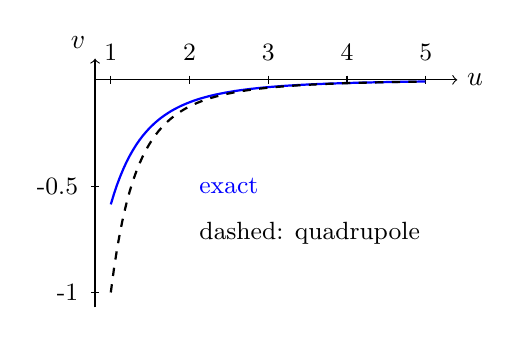
\begin{tikzpicture}[x=1.0cm,y=2.7cm]
\draw[->] (0.8,-1.07)--(0.8,0.1) node[above left] {$v$};
\draw[->] (0.8,0)--(5.4,0) node[right] {$u$};
\foreach \x in {1,2,3,4,5} {\draw (\x,0.02)--(\x,-0.02) node[above=5pt] {\small\x};}
\foreach \y in {-1,-0.5} {\draw (0.75,\y)--(0.85,\y) node[left=4pt] {\small\y};}
\draw[blue,thick,domain=1:5,samples=100] plot (\x,{2*(1/sqrt(\x*\x+1)-1/\x)});
\draw[dashed,thick,domain=1:5,samples=100] plot (\x,{-1/(\x*\x*\x)});
\node[blue,anchor=west] at (2,-0.5) {\small exact};
\node[anchor=west] at (2,-0.72) {\small dashed: quadrupole};
\end{tikzpicture}\hspace{1em}
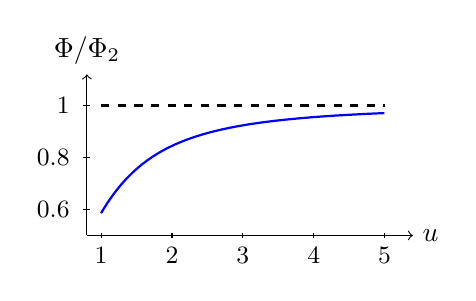
\begin{tikzpicture}[x=0.9cm,y=3.3cm]
\draw[->] (0.8,0.5)--(0.8,1.12) node[above] {$\Phi/\Phi_2$};
\draw[->] (0.8,0.5)--(5.4,0.5) node[right] {$u$};
\foreach \x in {1,2,3,4,5} {\draw (\x,0.51)--(\x,0.49) node[below] {\small\x};}
\foreach \y in {0.6,0.8,1} {\draw (0.75,\y)--(0.85,\y) node[left=4pt] {\small\y};}
\draw[dashed,thick] (1,1)--(5,1);
\draw[blue,thick,domain=1:5,samples=100]
plot (\x,{2/(sqrt(1+1/(\x*\x))*(1+sqrt(1+1/(\x*\x))))});
\end{tikzpicture}
\end{center}
For example the ratios at $u=2,3,5$ are $0.84458,0.92370,0.97097$.

\Needspace{5\baselineskip}
\par\bigskip
\noindent\textbf{4.2}\quad A point dipole with dipole moment $\mathbf{p}$ is located at the point $\mathbf{x}_{0}$. From the properties of the derivative of a Dirac delta function, show that for calculation of the potential $\Phi$ or the energy of a dipole in an external field, the dipole can be described by an effective charge density
\[
\rho_{\mathrm{eff}}(\mathbf{x})=-\mathbf{p}\cdot\nabla\delta(\mathbf{x}-\mathbf{x}_{0})
\]
\solution

The defining distributional identity is
\[
\int f(\mathbf x)\partial_i\delta(\mathbf x-\mathbf x_0)\,d^3x
=-\partial_i f(\mathbf x_0).
\]
Thus $\int\rho_{\rm eff}f\,d^3x=\mathbf p\cdot\nabla f(\mathbf x_0)$.
For an observation point $\mathbf r\ne\mathbf x_0$, put
$f(\mathbf x)=1/|\mathbf r-\mathbf x|$. The derivative is with respect
to the source coordinate, so
\[
\nabla_{\mathbf x}\frac1{|\mathbf r-\mathbf x|}
=\frac{\mathbf r-\mathbf x}{|\mathbf r-\mathbf x|^3},\qquad
\boxed{\Phi(\mathbf r)=\frac{1}{4\pi\epsilon_0}
\frac{\mathbf p\cdot(\mathbf r-\mathbf x_0)}{|\mathbf r-\mathbf x_0|^3}.}
\]
For the energy choose $f=\Phi^{(0)}$, smooth at $\mathbf x_0$. Since
this is interaction with distinct external sources, there is no factor $1/2$:
\[
\boxed{W=\int\rho_{\rm eff}\Phi^{(0)}\,d^3x
=\mathbf p\cdot\nabla\Phi^{(0)}(\mathbf x_0)
=-\mathbf p\cdot\mathbf E^{(0)}(\mathbf x_0).}
\]
Self-energy is excluded. Taking $f=1$ checks zero total charge;
taking $f=x_i$ checks $\int x_i\rho_{\rm eff}\,d^3x=p_i$.
For a further direct construction, place $\pm q$ a displacement
$\pm\mathbf d/2$ from $\mathbf x_0$. Taylor expansion gives
\[
q[\delta(\mathbf x-\mathbf x_0-\mathbf d/2)
-\delta(\mathbf x-\mathbf x_0+\mathbf d/2)]
=-q\mathbf d\cdot\nabla\delta(\mathbf x-\mathbf x_0)+O(qd^3).
\]
Taking $\mathbf d\to0$ with $q\mathbf d=\mathbf p$ fixed gives the
same density and fixes its sign.

\Needspace{5\baselineskip}
\par\bigskip
\noindent\textbf{4.3}\quad The $l$th term in the multipole expansion (4.1) of the potential is specified by the $(2l+1)$ multipole moments $q_{lm}$. On the other hand, the Cartesian multipole moments,
\[
Q_{\alpha\beta\gamma}^{(l)}=\int\rho(\mathbf{x})\,x^{\alpha}y^{\beta}z^{\gamma}\;d^{3}x
\]
with $\alpha$, $\beta$, $\gamma$ nonnegative integers subject to the constraint $\alpha+\beta+\gamma=l$, are $(l+1)(l+2)/2$ in number. Thus, for $l>1$ there are more Cartesian multipole moments than seem necessary to describe the term in the potential whose radial dependence is $r^{-l-1}$.

Show that while the $q_{lm}$ transform under rotations as irreducible spherical tensors of rank $l$, the Cartesian multipole moments correspond to reducible spherical tensors of ranks $l$, $l-2$, $l-4$, \ldots, $l_{\min}$, where $l_{\min}=0$ or 1 for $l$ even or odd, respectively. Check that the number of different tensorial components adds up to the total number of Cartesian tensors. Why are only the $q_{lm}$ needed in the expansion (4.1)?
\solution

Package the Cartesian moments into the symmetric rank-$l$ tensor
$M_{i_1\cdots i_l}=\int\rho x_{i_1}\cdots x_{i_l}\,d^3x$.
Its independent components correspond to homogeneous polynomials of degree
$l$, whose monomials are $x^\alpha y^\beta z^\gamma$ with
$\alpha+\beta+\gamma=l$. There are $\binom{l+2}{2}$ such monomials.

A homogeneous polynomial has the unique harmonic decomposition
\[
F_l(\mathbf x)=H_l(\mathbf x)+r^2H_{l-2}(\mathbf x)
+r^4H_{l-4}(\mathbf x)+\cdots,
\qquad \nabla^2H_k=0,
\]
where each $H_k$ is homogeneous of degree $k$. Here is why traces can
be removed recursively. For such a harmonic $H_k$, Euler's identity
$\mathbf x\cdot\nabla H_k=kH_k$ gives
\begin{align*}
\nabla^2(r^{2s}H_k)
&=(\nabla^2r^{2s})H_k+2\nabla r^{2s}\cdot\nabla H_k\\
&=[2s(2s+1)+4sk]r^{2s-2}H_k
=2s(2k+2s+1)r^{2s-2}H_k.
\end{align*}
The coefficient is nonzero for $s\geq1$. Decompose $\nabla^2F_l$
recursively and subtract the corresponding $r^{2s}H_k$ terms; the
remainder is harmonic. The same nonzero coefficients establish uniqueness.
In tensor language $H_l$ is the symmetric traceless part, while each
factor $r^2$ corresponds to a Kronecker delta, or trace.

The degree-$k$ harmonic polynomials have the basis
$\mathcal Y_{km}=r^kY_{km}$, $-k\leq m\leq k$.
Rotations preserve degree and harmonicity and mix only these $2k+1$
components. Moreover $L^2Y_{km}=k(k+1)Y_{km}$, and $L_\pm$ connect all
$m$ in that set; this is the irreducible rank-$k$ representation.
Therefore the Cartesian moments contain the ranks
\[
\boxed{l,\ l-2,\ l-4,\ldots,l_{\min},}
\]
whereas the integrals $q_{lm}=\int\rho\mathcal Y_{lm}^{*}\,d^3x$
select just the irreducible rank-$l$ part. The lower-rank pieces of
$M^{(l)}$ involve radial weights $r^{2s}$; they are not generally the
ordinary moments of order $l-2s$.

For $l=2n$, the number of components is
\[
\sum_{k=0}^n(4k+1)=(n+1)(2n+1)
=\frac{(l+1)(l+2)}2;
\]
for $l=2n+1$ it is
\[
\sum_{k=0}^n(4k+3)=(n+1)(2n+3)
=\frac{(l+1)(l+2)}2.
\]
Finally, Taylor expansion of the Coulomb kernel yields
\[
\Phi_l(\mathbf r)=\frac{1}{4\pi\epsilon_0}
\frac{(-1)^l}{l!}M_{i_1\cdots i_l}
\partial_{i_1}\cdots\partial_{i_l}\frac1r.
\]
Any trace in $M$ contracts two derivatives into
$\nabla^2(1/r)=0$ at exterior points. Only its symmetric traceless
part contributes, and that part is fully specified by the $2l+1$
$q_{lm}$. This explains why the extra Cartesian components do not
appear in (4.1).

\Needspace{5\baselineskip}
\par\bigskip
\noindent\textbf{4.4}\quad\begin{enumerate}
\item[(a)] Prove the following theorem: For an arbitrary charge distribution $\rho(\mathbf{x})$ the values of the $(2l+1)$ moments of the first nonvanishing multipole are independent of the origin of the coordinate axes, but the values of all higher multipole moments do in general depend on the choice of origin. (The different moments $q_{lm}$ for fixed $l$ depend, of course, on the orientation of the axes.)
\item[(b)] A charge distribution has multipole moments $q$, $\mathbf{p}$, $Q_{ij}$, \ldots{} with respect to one set of coordinate axes, and moments $q'$, $\mathbf{p}'$, $Q'_{ij}$, \ldots{} with respect to another set whose axes are parallel to the first, but whose origin is located at the point $\mathbf{R}=(X,Y,Z)$ relative to the first. Determine explicitly the connections between the monopole, dipole, and quadrupole moments in the two coordinate frames.
\item[(c)] If $q\neq0$, can $\mathbf{R}$ be found so that $\mathbf{p}'=0$? If $q\neq0$, $\mathbf{p}\neq0$, or at least $\mathbf{p}\neq0$, can $\mathbf{R}$ be found so that $Q'_{ij}=0$?
\end{enumerate}
\solution

\textbf{(a)} Keep the axes parallel and move the origin to $\mathbf R$,
so that $\mathbf x'=\mathbf x-\mathbf R$. For the regular solid harmonic
$\mathcal Y_{lm}=r^lY_{lm}$, the finite Taylor expansion is
\[
\mathcal Y_{lm}^{*}(\mathbf x-\mathbf R)
=\sum_{k=0}^l\frac{(-\mathbf R\cdot\nabla)^k}{k!}
\mathcal Y_{lm}^{*}(\mathbf x).
\]
Each derivative on the right is a homogeneous polynomial of degree
$l-k$ and is harmonic, since differentiation commutes with $\nabla^2$.
It is consequently a linear combination of the $\mathcal Y_{l-k,m'}$.
Multiplying by $\rho$ and integrating shows that
\[
q'_{lm}=q_{lm}+\text{linear combinations of moments of orders }0,\ldots,l-1.
\]
If all moments below order $L$ vanish, then $q'_{Lm}=q_{Lm}$ and all
moments below $L$ remain zero. Higher moments contain terms involving
the nonzero order-$L$ moments, so in general they change under
translation. Particular components may be unchanged for particular
translations; the theorem does not assert otherwise. Rotations still
mix the $m$ components within each order.

\textbf{(b)} With $q=\int\rho\,d^3x$, $p_i=\int\rho x_i\,d^3x$, and
$Q_{ij}=\int\rho(3x_ix_j-r^2\delta_{ij})\,d^3x$,
\[
\boxed{q'=q,\qquad p'_i=p_i-qR_i.}
\]
For the quadrupole, expand its integrand before integrating:
\begin{align*}
3(x_i-R_i)(x_j-R_j)-|\mathbf x-\mathbf R|^2\delta_{ij}
={}&3x_ix_j-r^2\delta_{ij}-3(R_ix_j+R_jx_i)\\
&+2(\mathbf R\cdot\mathbf x)\delta_{ij}
+3R_iR_j-R^2\delta_{ij}.
\end{align*}
Thus
\[
\boxed{Q'_{ij}=Q_{ij}-3(R_ip_j+R_jp_i)
+2\mathbf R\cdot\mathbf p\,\delta_{ij}
+q(3R_iR_j-R^2\delta_{ij}).}
\]
The trace remains zero, as it must.

\textbf{(c)} If $q\ne0$, the unique dipole-free origin is
$\boxed{\mathbf R=\mathbf p/q}$. A quadrupole-free origin generally does
not exist. To give the precise restriction, define the quadrupole at
this dipole-free origin,
\[
Q^{c}_{ij}=Q_{ij}-\frac{3p_ip_j-p^2\delta_{ij}}q,
\qquad \mathbf s=\mathbf R-\frac{\mathbf p}q.
\]
Completing the square in the transformation law gives
\[
Q'_{ij}=Q^c_{ij}+q(3s_is_j-s^2\delta_{ij}).
\]
The matrix $3\mathbf s\mathbf s^{\mathsf T}-s^2\mathbf I$ has
eigenvalue $2s^2$ along $\mathbf s$ and $-s^2$ along each perpendicular
direction; this identifies the possible spectra of its negative.
Therefore $Q'=0$ is possible exactly when $Q^c=0$ (choose $\mathbf s=0$),
or when $Q^c$ has eigenvalues $(-2\lambda,\lambda,\lambda)$ with
$\lambda/q>0$. The direction of $\mathbf s$ must be the first
principal axis, and $s^2=\lambda/q$. A generic traceless symmetric
tensor has three distinct eigenvalues and fails this condition.
For example, equal pairs of charges $+e$ at $\pm a\hat{\mathbf x}$ and
$+2e$ at $\pm a\hat{\mathbf y}$ have $q=6e$, $\mathbf p=0$, and
$Q^c=6ea^2\operatorname{diag}(0,1,-1)$, which cannot be removed by
translation. Describing this same distribution from another origin
makes $\mathbf p\ne0$ without removing the obstruction.

If $q=0$ but $\mathbf p\ne0$, choose axes with $\mathbf p=p\hat{\mathbf z}$.
The six symmetric components transform as
\begin{gather*}
Q'_{xx}=Q_{xx}+2pR_z,\quad Q'_{yy}=Q_{yy}+2pR_z,\quad
Q'_{zz}=Q_{zz}-4pR_z,\\
Q'_{xy}=Q_{xy},\quad Q'_{xz}=Q_{xz}-3pR_x,\quad
Q'_{yz}=Q_{yz}-3pR_y.
\end{gather*}
Thus $Q'=0$ requires $Q_{xy}=0$ and $Q_{xx}=Q_{yy}$; when these
conditions hold, choose
\[
(R_x,R_y,R_z)=\left(\frac{Q_{xz}}{3p},\frac{Q_{yz}}{3p},
-\frac{Q_{xx}}{2p}\right).
\]
If both $q$ and $\mathbf p$ vanish, the quadrupole is invariant and
can be zero in a translated frame only if it was zero already.

\Needspace{5\baselineskip}
\par\bigskip
\noindent\textbf{4.5}\quad A localized charge density $\rho(x,y,z)$ is placed in an external electrostatic field described by a potential $\Phi^{(0)}(x,y,z)$. The external potential varies slowly in space over the region where the charge density is different from zero. \erratum{Assume that the external sources lie outside a neighborhood of this region, so that $\nabla^2\Phi^{(0)}=0$ there, as in the derivation of (4.23)--(4.24).}
\begin{enumerate}
\item[(a)] From first principles calculate the total \emph{force} acting on the charge distribution as an expansion in multipole moments times derivatives of the electric field, up to and including the quadrupole moments. Show that the force is
\[
\mathbf{F}=q\mathbf{E}^{(0)}(0)+\{\nabla[\mathbf{p}\cdot\mathbf{E}^{(0)}(\mathbf{x})]\}_{0}+\left\{\nabla\!\left[\frac{1}{6}\sum_{j,k}Q_{jk}\frac{\partial E_{j}^{(0)}}{\partial x_{k}}(\mathbf{x})\right]\right\}_{0}+\cdots
\]
Compare this to the expansion (4.24) of the \emph{energy} $W$. Note that (4.24) is a number---it is not a function of $\mathbf{x}$ that can be differentiated! What is its connection to $\mathbf{F}$?
\item[(b)] Repeat the calculation of part a for the total \emph{torque}. For simplicity, evaluate only one Cartesian component of the torque, say $N_{1}$. Show that this component is
\[
N_{1}=[\mathbf{p}\times\mathbf{E}^{(0)}(0)]_{1}+\frac{1}{3}\left[\frac{\partial}{\partial x_{3}}\left(\sum_{j}Q_{2j}E_{j}^{(0)}\right)-\frac{\partial}{\partial x_{2}}\left(\sum_{j}Q_{3j}E_{j}^{(0)}\right)\right]_{0}+\cdots
\]
\end{enumerate}
\solution

As in Jackson's derivation of (4.23)--(4.24), assume that the external
sources lie outside a neighborhood containing the localized distribution.
Then $\nabla\cdot\mathbf E^{(0)}=0$ and
$\nabla\times\mathbf E^{(0)}=0$ there. This source-free condition is
needed for the stated force formula with only traceless moments.
All derivatives below are of the external field.

\textbf{(a)} Start with the force on each charge element:
\[
F_i=\int\rho(\mathbf x)E_i^{(0)}(\mathbf x)\,d^3x.
\]
Taylor-expand the field around the origin, integrate term by term,
and define $M_{jk}=\int\rho x_jx_k\,d^3x$ and
$S=\int\rho r^2\,d^3x$:
\begin{align*}
F_i&=qE_i^{(0)}(0)+p_j\partial_jE_i^{(0)}(0)
+\frac12M_{jk}\partial_j\partial_kE_i^{(0)}(0)+\cdots,\\
M_{jk}&=\frac13(Q_{jk}+S\delta_{jk}).
\end{align*}
The trace term is $S\nabla^2E_i^{(0)}/6=0$, because
$\nabla^2\mathbf E^{(0)}=\nabla(\nabla\cdot\mathbf E^{(0)})=0$.
Electrostatics also gives $\partial_jE_i^{(0)}=\partial_iE_j^{(0)}$,
so
\begin{align*}
p_j\partial_jE_i^{(0)}&=\partial_i(p_jE_j^{(0)}),\\
Q_{jk}\partial_j\partial_kE_i^{(0)}
&=\partial_i(Q_{jk}\partial_kE_j^{(0)}).
\end{align*}
These identities give exactly
\[
\boxed{\mathbf F=q\mathbf E^{(0)}(0)
+\left.\nabla(\mathbf p\cdot\mathbf E^{(0)})\right|_0
+\left.\frac16\nabla(Q_{jk}\partial_kE_j^{(0)})\right|_0+\cdots.}
\]
Repeated Cartesian indices are summed. If external charge overlaps the
region, the additional term $S\nabla(\nabla\cdot\mathbf E^{(0)})/6$
must be retained; the displayed problem formula alone is then insufficient.

To connect force and energy, let $\mathbf R$ be a \emph{physical rigid
translation} of the charge distribution and let $\mathbf u$ denote
coordinates fixed in it. Its interaction energy is the function
\begin{align*}
W(\mathbf R)&=\int\rho(\mathbf u)\Phi^{(0)}(\mathbf R+\mathbf u)\,d^3u\\
&=q\Phi^{(0)}(\mathbf R)-p_jE_j^{(0)}(\mathbf R)
-\frac16Q_{jk}\partial_kE_j^{(0)}(\mathbf R)+\cdots.
\end{align*}
The moments are held fixed while differentiating, and
$\mathbf F=-\nabla_{\mathbf R}W(\mathbf R)|_{\mathbf R=0}$.
Equation (4.24) is the value $W(0)$, not a spatial function to which
one may directly apply $\nabla_{\mathbf x}$.

\textbf{(b)} The torque about the chosen origin is
\[
N_1=\int\rho(x_2E_3^{(0)}-x_3E_2^{(0)})\,d^3x.
\]
Keeping the constant and linear terms of the field produces
\begin{align*}
N_1={}&p_2E_3^{(0)}(0)-p_3E_2^{(0)}(0)
+M_{2j}\partial_jE_3^{(0)}(0)-M_{3j}\partial_jE_2^{(0)}(0)+\cdots\\
={}&[\mathbf p\times\mathbf E^{(0)}(0)]_1
+\frac13[Q_{2j}\partial_jE_3^{(0)}-Q_{3j}\partial_jE_2^{(0)}]_0
+\frac S3[\partial_2E_3^{(0)}-\partial_3E_2^{(0)}]_0+\cdots.
\end{align*}
The last term vanishes by zero curl. Interchanging the derivative and
field indices in the preceding term then gives
\[
\boxed{N_1=[\mathbf p\times\mathbf E^{(0)}(0)]_1
+\frac13[\partial_3(Q_{2j}E_j^{(0)})
-\partial_2(Q_{3j}E_j^{(0)})]_0+\cdots.}
\]
This torque is about the origin; about a different point it changes by
the usual moment of the total force.

\Needspace{5\baselineskip}
\par\bigskip
\noindent\textbf{4.6}\quad A nucleus with quadrupole moment $Q$ finds itself in a cylindrically symmetric electric field with a gradient $(\partial E_{z}/\partial z)_{0}$ along the $z$ axis at the position of the nucleus. \erratum{Take the nuclear symmetry axis along $z$ and the external field to be source-free at the nucleus; these conditions specify the aligned quadrupole energy below.}
\begin{enumerate}
\item[(a)] Show that the energy of quadrupole interaction is
\[
W=-\frac{e}{4}\,Q\left(\frac{\partial E_{z}}{\partial z}\right)_{0}
\]
\item[(b)] If it is known that $Q=2\times10^{-28}$ m$^{2}$ and that $W/h$ is 10 MHz, where $h$ is Planck's constant, calculate $(\partial E_{z}/\partial z)_{0}$ in units of $e/4\pi\epsilon_{0}a_{0}^{3}$, where $a_{0}=4\pi\epsilon_{0}\hbar^{2}/me^{2}=0.529\times10^{-10}$ m is the Bohr radius in hydrogen.
\item[(c)] Nuclear charge distributions can be approximated by a constant charge density throughout a spheroidal volume of semimajor axis $a$ and semiminor axis $b$. Calculate the quadrupole moment of such a nucleus, assuming that the total charge is $Ze$. Given that Eu$^{153}$ ($Z=63$) has a quadrupole moment $Q=2.5\times10^{-28}$ m$^{2}$ and a mean radius
\[
R=(a+b)/2=7\times10^{-15}\ \mathrm{m}
\]
determine the fractional difference in radius $(a-b)/R$.
\end{enumerate}
\solution

\textbf{(a)} Jackson's nuclear convention (4.25) is
$Q=Q_{zz}/e$, with dimensions of area. Take the nuclear symmetry axis
along $z$, as in that definition. Axial symmetry and tracelessness give
\[
Q_{zz}=eQ,\qquad Q_{xx}=Q_{yy}=-eQ/2,\qquad Q_{ij}=0\ (i\ne j).
\]
At a source-free point of an axially symmetric external field, let
$G=(\partial_zE_z)_0$. Then
$\partial_xE_x=\partial_yE_y$ and
$\partial_xE_x+\partial_yE_y+\partial_zE_z=0$, so each transverse
entry is $-G/2$. Thus
\[
W_Q=-\frac16 Q_{ij}\partial_jE_i
=-\frac16\left[eQG+2\left(-\frac{eQ}{2}\right)
\left(-\frac G2\right)\right]
=\boxed{-\frac{eQG}{4}}.
\]
For a nucleus whose symmetry axis makes angle $\beta$ with the field
axis, write $Q_{ij}=eQ(3\widehat u_i\widehat u_j-\delta_{ij})/2$,
where $\widehat{\mathbf u}\cdot\widehat{\mathbf z}=\cos\beta$.
The traceless gradient tensor is
$G_{ij}=G(3\widehat z_i\widehat z_j-\delta_{ij})/2$. Thus
\[
-\frac16Q_{ij}G_{ij}
=-\frac{eQG}{24}(9\cos^2\beta-3)
=-\frac{eQG}{4}P_2(\cos\beta).
\]
The stated formula uses the aligned convention $\beta=0$.

\textbf{(b)} With $W/h=+10^7\ \mathrm{s}^{-1}$ and $Q>0$,
\[
G=-\frac{4h(10^7\ \mathrm{s}^{-1})}{e(2\times10^{-28}\ \mathrm{m}^2)}
=-8.2713\times10^{20}\ \mathrm{V\,m^{-2}}.
\]
Using the problem's rounded $a_0=0.529\times10^{-10}\ \mathrm m$,
\[
\frac{e}{4\pi\epsilon_0a_0^3}=9.7271\times10^{21}\ \mathrm{V\,m^{-2}},
\qquad
\boxed{\frac{G}{e/(4\pi\epsilon_0a_0^3)}=-0.08503.}
\]
If the measured $10$ MHz denotes only the magnitude of a splitting,
only $|G|$ is determined and the ratio is $0.08503$ in magnitude.

\textbf{(c)} For a prolate spheroid put the semiaxis $a$ along $z$
and the equal semiaxes $b$ along $x,y$. Its density is
$\rho=3Ze/(4\pi ab^2)$. Transform the ellipsoid to the unit ball by
$x=bu$, $y=bv$, $z=aw$. Spherical symmetry on that ball gives
\[
\int_{u^2+v^2+w^2\leq1}w^2\,d^3u
=\frac13\int_0^1 4\pi t^4\,dt=\frac{4\pi}{15}.
\]
Since $d^3x=ab^2d^3u$,
\[
\int\rho z^2\,d^3x=\frac{Ze a^2}{5},\qquad
\int\rho x^2\,d^3x=\int\rho y^2\,d^3x=\frac{Ze b^2}{5}.
\]
It follows that
\[
\boxed{Q=\frac1e\int\rho(2z^2-x^2-y^2)\,d^3x
=\frac{2Z}{5}(a^2-b^2).}
\]
For an oblate spheroid the axial semiaxis is the smaller one, and the
quadrupole has the opposite sign. Here $Q>0$ selects the prolate case.
Using $a+b=2R$, with no small-deformation approximation,
\[
Q=\frac{4Z}{5}R(a-b),\qquad
\boxed{\frac{a-b}{R}=\frac{5Q}{4ZR^2}
=\frac{5(2.5\times10^{-28})}{4(63)(7\times10^{-15})^2}
=0.10123.}
\]
Thus $a\simeq7.354\times10^{-15}$ m and
$b\simeq6.646\times10^{-15}$ m in this uniform-density model.

\Needspace{5\baselineskip}
\par\bigskip
\noindent\textbf{4.7}\quad A localized distribution of charge has a charge density
\[
\rho(\mathbf{r})=\frac{1}{64\pi}\,r^{2}e^{-r}\sin^{2}\theta
\]
\begin{enumerate}
\item[(a)] Make a multipole expansion of the potential due to this charge density and determine all the nonvanishing multipole moments. Write down the potential at large distances as a finite expansion in Legendre polynomials.
\item[(b)] Determine the potential explicitly at any point in space, and show that near the origin, correct to $r^{2}$ inclusive,
\[
\Phi(\mathbf{r})\simeq\frac{1}{4\pi\epsilon_{0}}\left[\frac{1}{4}-\frac{r^{2}}{120}P_{2}(\cos\theta)\right]
\]
\item[(c)] If there exists at the origin a nucleus with a quadrupole moment $Q=10^{-28}$ m$^{2}$, \erratum{with its symmetry axis along $z$,} determine the magnitude of the interaction energy, assuming that the unit of charge in $\rho(\mathbf{r})$ above is the electronic charge and the unit of length is the hydrogen Bohr radius $a_{0}=4\pi\epsilon_{0}\hbar^{2}/me^{2}=0.529\times10^{-10}$ m. Express your answer as a frequency by dividing by Planck's constant $h$.
\end{enumerate}
The charge density in this problem is that for the $m=\pm1$ states of the $2p$ level in hydrogen, while the quadrupole interaction is of the same order as found in molecules.
\solution

\textbf{(a)} Use $\sin^2\theta=\frac23[1-P_2(\cos\theta)]$ to write
\[
\rho=\frac{r^2e^{-r}}{96\pi}[1-P_2(\cos\theta)].
\]
Azimuthal integration eliminates $m\ne0$, and Legendre orthogonality
eliminates $l\ne0,2$. Since
$\int_0^\infty r^ne^{-r}\,dr=n!$ and
$\int P_l^2\,d\Omega=4\pi/(2l+1)$, the total charge and the
Legendre quadrupole integral are
\[
q=\frac{4\pi}{96\pi}\,4!=1,\qquad
\int\rho r^2P_2\,d^3r=-\frac{1}{96\pi}\frac{4\pi}{5}\,6!=-6.
\]
Therefore
\[
\boxed{q_{00}=\frac1{\sqrt{4\pi}},\qquad
q_{20}=-6\sqrt{\frac5{4\pi}}=-3\sqrt{\frac5\pi},}
\]
with all other moments zero. The large-distance expansion is
\[
\boxed{\Phi\sim\frac{1}{4\pi\epsilon_0}
\left[\frac1r-\frac6{r^3}P_2(\cos\theta)\right].}
\]
The density is exponentially localized but is not compactly supported.
Consequently this finite algebraic expansion is asymptotic, with
exponentially small corrections at finite $r$; it is not the exact
potential throughout an exterior charge-free region.

\textbf{(b)} Split the Coulomb integral into source radii $s<r$ and
$s>r$, using the kernel $r_<^l/r_>^{l+1}$. The same angular
orthogonality gives
\[
4\pi\epsilon_0\Phi=A(r)+B(r)P_2(\cos\theta),
\]
\begin{align*}
A(r)&=\frac1{24}\left[\frac1r\int_0^r s^4e^{-s}\,ds
+\int_r^\infty s^3e^{-s}\,ds\right],\\
B(r)&=-\frac1{120}\left[\frac1{r^3}\int_0^r s^6e^{-s}\,ds
+r^2\int_r^\infty se^{-s}\,ds\right].
\end{align*}
Repeated integration by parts gives
\[
\int_r^\infty s^ne^{-s}\,ds=n!e^{-r}\sum_{k=0}^n\frac{r^k}{k!},
\qquad
\int_0^r s^ne^{-s}\,ds=n!\left[1-e^{-r}\sum_{k=0}^n\frac{r^k}{k!}\right].
\]
Substituting and collecting equal powers yields the explicit answer
\begin{align*}
\boxed{A(r)}&=\boxed{\frac1r-e^{-r}\left(\frac1r+\frac34+\frac r4+\frac{r^2}{24}\right)},\\
\boxed{B(r)}&=\boxed{-\frac6{r^3}+e^{-r}\left(\frac6{r^3}+\frac6{r^2}
+\frac3r+1+\frac r4+\frac{r^2}{24}\right)}.
\end{align*}
These expressions apply for $r>0$; their apparent singularities are
removable at the origin. The integral forms show the cancellations
without subtracting divergent terms. For small $r$, the needed integrals are
\begin{gather*}
\int_0^r s^4e^{-s}\,ds=\frac{r^5}{5}+O(r^6),\qquad
\int_r^\infty s^3e^{-s}\,ds=6-\frac{r^4}{4}+O(r^5),\\
\int_0^r s^6e^{-s}\,ds=\frac{r^7}{7}+O(r^8),\qquad
\int_r^\infty se^{-s}\,ds=1-\frac{r^2}{2}+O(r^3).
\end{gather*}
Consequently
\begin{align*}
A(r)&=\frac1{24}\left[6+\left(\frac15-\frac14\right)r^4+O(r^5)\right]
=\frac14-\frac{r^4}{480}+O(r^5),\\
B(r)&=-\frac1{120}\left[r^2+\left(\frac17-\frac12\right)r^4+O(r^5)\right]
=-\frac{r^2}{120}+\frac{r^4}{336}+O(r^5),
\end{align*}
so
\[
\boxed{\Phi=\frac{1}{4\pi\epsilon_0}
\left[\frac14-\frac{r^2}{120}P_2(\cos\theta)+O(r^4)\right].}
\]
For example, differentiating the exact radial functions checks Poisson's
 equation directly:
\[
A''+\frac2rA'=-\frac{r^2e^{-r}}{24},\qquad
B''+\frac2rB'-\frac6{r^2}B=+\frac{r^2e^{-r}}{24}.
\]

\textbf{(c)} Restore physical length $\mathbf R=a_0\mathbf r$ and
charge $q_e$ (equal to $-e$ for an electron). The quadratic physical
potential is
\[
\Phi_Q(\mathbf R)=-\frac{q_e}{4\pi\epsilon_0a_0^3}
\frac{3Z^2-R^2}{240}.
\]
Since $3Z^2-R^2=2Z^2-X^2-Y^2$,
\[
\left(\frac{\partial E_Z}{\partial Z}\right)_0
=-\partial_Z^2\Phi_Q=\frac{q_e}{4\pi\epsilon_0a_0^3}\frac1{60}.
\]
For the nuclear quadrupole convention and alignment of Problem 4.6,
\[
|W_Q|=\frac{e^2|Q|}{240(4\pi\epsilon_0)a_0^3},\qquad
\boxed{\frac{|W_Q|}{h}=9.8000\times10^5\ \mathrm{Hz}\simeq0.980\ \mathrm{MHz}.}
\]
The sign reverses if the sign of the charge distribution is reversed;
for an electron and $Q>0$, this aligned quadrupole contribution is positive.

\Needspace{5\baselineskip}
\par\bigskip
\noindent\textbf{4.8}\quad A very long, right circular, cylindrical shell of dielectric constant $\epsilon/\epsilon_{0}$ and inner and outer radii $a$ and $b$, respectively, is placed in a previously uniform electric field $E_{0}$ with its axis perpendicular to the field. The medium inside and outside the cylinder has a dielectric constant of unity.
\begin{enumerate}
\item[(a)] Determine the potential and electric field in the three regions, neglecting end effects.
\item[(b)] Sketch the lines of force for a typical case of $b\simeq2a$.
\item[(c)] Discuss the limiting forms of your solution appropriate for a solid dielectric cylinder in a uniform field, and a cylindrical cavity in a uniform dielectric.
\end{enumerate}
\solution

\textbf{(a)} Let $\kappa=\epsilon/\epsilon_0>0$, use cylindrical
coordinates $(s,\phi,z)$, and take the applied field along $x$, so
$x=s\cos\phi$. Translation invariance along $z$ and the $\cos\phi$
boundary condition leave only the cylindrical harmonic of order one.
The solutions regular at $s=0$ and asymptotic to $-E_0x$ are
\[
\Phi=-E_0\cos\phi\begin{cases}
As,&s<a,\\
Bs+C/s,&a<s<b,\\
s-D/s,&s>b.
\end{cases}
\]
There is no free surface charge at either dielectric boundary. Continuity
of $\Phi$ and of $D_s=-\epsilon\partial_s\Phi$ gives four equations:
\begin{gather*}
A=B+C/a^2,\qquad A=\kappa(B-C/a^2),\\
B+C/b^2=1-D/b^2,\qquad
\kappa(B-C/b^2)=1+D/b^2.
\end{gather*}
The first pair gives
$C=a^2B(\kappa-1)/(\kappa+1)$ and
$A=2\kappa B/(\kappa+1)$. Adding the second pair eliminates $D$:
\[
(\kappa+1)B-(\kappa-1)C/b^2=2.
\]
Define $\eta=a^2/b^2$ and
$\Delta=(\kappa+1)^2-(\kappa-1)^2\eta$. Substitution gives
\[
\boxed{A=\frac{4\kappa}{\Delta},\quad
B=\frac{2(\kappa+1)}{\Delta},\quad
C=\frac{2(\kappa-1)a^2}{\Delta},\quad
D=\frac{(\kappa^2-1)(b^2-a^2)}{\Delta}.}
\]
The field is $\mathbf E=E_s\hat{\mathbf s}+E_\phi\hat{\boldsymbol\phi}$,
with $E_z=0$ and
\[
\boxed{\frac{E_s}{E_0}=\cos\phi\begin{cases}
A,&s<a,\\ B-C/s^2,&a<s<b,\\1+D/s^2,&s>b,
\end{cases}\quad
\frac{E_\phi}{E_0}=-\sin\phi\begin{cases}
A,&s<a,\\B+C/s^2,&a<s<b,\\1-D/s^2,&s>b.
\end{cases}}
\]
Thus the field in the hollow core is uniform, $\mathbf E=AE_0\hat{\mathbf x}$.
For $\kappa=1$, $A=B=1$ and $C=D=0$, recovering a uniform vacuum field.

\textbf{(b)} The field lines are contours of a stream function.
In each homogeneous region introduce the stream
function for $\mathbf D/(\epsilon_0E_0)$:
\[
\Psi(s,\phi)=\sin\phi\begin{cases}
As,&s<a,\\
\kappa(Bs-C/s),&a<s<b,\\
s+D/s,&s>b.
\end{cases}
\]
It obeys $D_s/(\epsilon_0E_0)=s^{-1}\partial_\phi\Psi$ and
$D_\phi/(\epsilon_0E_0)=-\partial_s\Psi$. Hence
$\mathbf E\cdot\nabla\Psi=0$, and contours of $\Psi$ are field lines.
The boundary equations above make $\Psi$ continuous across both circles.
The direction changes there in accordance with continuous $E_\phi$
and $\epsilon E_s$.

The plot uses $b=2a$, $\kappa=4$:
$A=64/91$, $B=40/91$, $C/a^2=24/91$, $D/a^2=180/91$.
The shaded annulus is the dielectric, and arrows point along the field.
\begin{center}
% Generated by supplementary/check_ch04.py --figures.
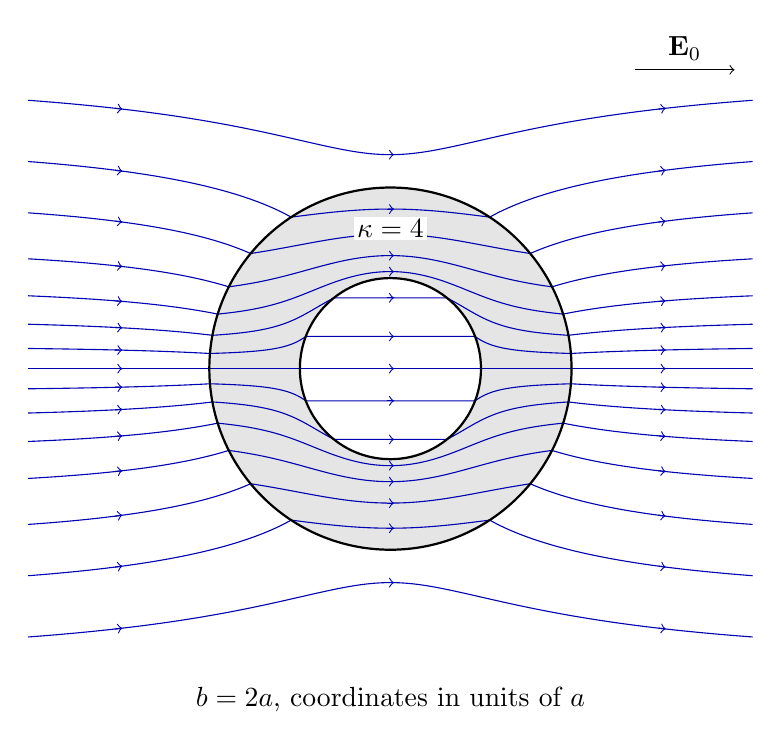
\begin{tikzpicture}[scale=1.15]
\fill[gray!20] (0,0) circle (2);
\fill[white] (0,0) circle (1);
\draw[blue!70!black,thin] plot coordinates {(-4.0000,-2.96347) (-3.9800,-2.96197) (-3.9600,-2.96046) (-3.9400,-2.95893) (-3.9200,-2.95740) (-3.9000,-2.95585) (-3.8800,-2.95429) (-3.8600,-2.95271) (-3.8400,-2.95112) (-3.8200,-2.94952) (-3.8000,-2.94790) (-3.7800,-2.94627) (-3.7600,-2.94463) (-3.7400,-2.94298) (-3.7200,-2.94131) (-3.7000,-2.93962) (-3.6800,-2.93792) (-3.6600,-2.93621) (-3.6400,-2.93448) (-3.6200,-2.93274) (-3.6000,-2.93098) (-3.5800,-2.92921) (-3.5600,-2.92742) (-3.5400,-2.92562) (-3.5200,-2.92380) (-3.5000,-2.92197) (-3.4800,-2.92012) (-3.4600,-2.91825) (-3.4400,-2.91637) (-3.4200,-2.91448) (-3.4000,-2.91256) (-3.3800,-2.91063) (-3.3600,-2.90869) (-3.3400,-2.90672) (-3.3200,-2.90474) (-3.3000,-2.90275) (-3.2800,-2.90073) (-3.2600,-2.89870) (-3.2400,-2.89665) (-3.2200,-2.89459) (-3.2000,-2.89250) (-3.1800,-2.89040) (-3.1600,-2.88828) (-3.1400,-2.88614) (-3.1200,-2.88399) (-3.1000,-2.88181) (-3.0800,-2.87962) (-3.0600,-2.87740) (-3.0400,-2.87517) (-3.0200,-2.87292) (-3.0000,-2.87065) (-2.9800,-2.86836) (-2.9600,-2.86605) (-2.9400,-2.86372) (-2.9200,-2.86137) (-2.9000,-2.85900) (-2.8800,-2.85660) (-2.8600,-2.85419) (-2.8400,-2.85176) (-2.8200,-2.84931) (-2.8000,-2.84683) (-2.7800,-2.84433) (-2.7600,-2.84182) (-2.7400,-2.83928) (-2.7200,-2.83671) (-2.7000,-2.83413) (-2.6800,-2.83152) (-2.6600,-2.82889) (-2.6400,-2.82624) (-2.6200,-2.82357) (-2.6000,-2.82087) (-2.5800,-2.81815) (-2.5600,-2.81541) (-2.5400,-2.81264) (-2.5200,-2.80985) (-2.5000,-2.80704) (-2.4800,-2.80420) (-2.4600,-2.80133) (-2.4400,-2.79845) (-2.4200,-2.79553) (-2.4000,-2.79260) (-2.3800,-2.78963) (-2.3600,-2.78665) (-2.3400,-2.78364) (-2.3200,-2.78060) (-2.3000,-2.77754) (-2.2800,-2.77445) (-2.2600,-2.77133) (-2.2400,-2.76819) (-2.2200,-2.76502) (-2.2000,-2.76183) (-2.1800,-2.75861) (-2.1600,-2.75537) (-2.1400,-2.75209) (-2.1200,-2.74879) (-2.1000,-2.74547) (-2.0800,-2.74211) (-2.0600,-2.73873) (-2.0400,-2.73532) (-2.0200,-2.73189) (-2.0000,-2.72842) (-1.9800,-2.72493) (-1.9600,-2.72141) (-1.9400,-2.71786) (-1.9200,-2.71429) (-1.9000,-2.71069) (-1.8800,-2.70706) (-1.8600,-2.70340) (-1.8400,-2.69971) (-1.8200,-2.69600) (-1.8000,-2.69226) (-1.7800,-2.68849) (-1.7600,-2.68469) (-1.7400,-2.68086) (-1.7200,-2.67701) (-1.7000,-2.67313) (-1.6800,-2.66922) (-1.6600,-2.66528) (-1.6400,-2.66131) (-1.6200,-2.65732) (-1.6000,-2.65330) (-1.5800,-2.64926) (-1.5600,-2.64519) (-1.5400,-2.64109) (-1.5200,-2.63696) (-1.5000,-2.63281) (-1.4800,-2.62863) (-1.4600,-2.62443) (-1.4400,-2.62021) (-1.4200,-2.61596) (-1.4000,-2.61168) (-1.3800,-2.60738) (-1.3600,-2.60306) (-1.3400,-2.59872) (-1.3200,-2.59435) (-1.3000,-2.58997) (-1.2800,-2.58556) (-1.2600,-2.58114) (-1.2400,-2.57669) (-1.2200,-2.57223) (-1.2000,-2.56775) (-1.1800,-2.56326) (-1.1600,-2.55875) (-1.1400,-2.55423) (-1.1200,-2.54969) (-1.1000,-2.54515) (-1.0800,-2.54059) (-1.0600,-2.53603) (-1.0400,-2.53146) (-1.0200,-2.52689) (-1.0000,-2.52231) (-0.9800,-2.51773) (-0.9600,-2.51315) (-0.9400,-2.50858) (-0.9200,-2.50401) (-0.9000,-2.49945) (-0.8800,-2.49490) (-0.8600,-2.49036) (-0.8400,-2.48583) (-0.8200,-2.48132) (-0.8000,-2.47684) (-0.7800,-2.47237) (-0.7600,-2.46794) (-0.7400,-2.46353) (-0.7200,-2.45916) (-0.7000,-2.45482) (-0.6800,-2.45053) (-0.6600,-2.44628) (-0.6400,-2.44208) (-0.6200,-2.43794) (-0.6000,-2.43385) (-0.5800,-2.42982) (-0.5600,-2.42587) (-0.5400,-2.42198) (-0.5200,-2.41817) (-0.5000,-2.41444) (-0.4800,-2.41080) (-0.4600,-2.40726) (-0.4400,-2.40381) (-0.4200,-2.40046) (-0.4000,-2.39722) (-0.3800,-2.39409) (-0.3600,-2.39109) (-0.3400,-2.38821) (-0.3200,-2.38546) (-0.3000,-2.38284) (-0.2800,-2.38037) (-0.2600,-2.37804) (-0.2400,-2.37586) (-0.2200,-2.37384) (-0.2000,-2.37197) (-0.1800,-2.37027) (-0.1600,-2.36874) (-0.1400,-2.36738) (-0.1200,-2.36619) (-0.1000,-2.36518) (-0.0800,-2.36436) (-0.0600,-2.36371) (-0.0400,-2.36325) (-0.0200,-2.36297) (0.0000,-2.36287) (0.0200,-2.36297) (0.0400,-2.36325) (0.0600,-2.36371) (0.0800,-2.36436) (0.1000,-2.36518) (0.1200,-2.36619) (0.1400,-2.36738) (0.1600,-2.36874) (0.1800,-2.37027) (0.2000,-2.37197) (0.2200,-2.37384) (0.2400,-2.37586) (0.2600,-2.37804) (0.2800,-2.38037) (0.3000,-2.38284) (0.3200,-2.38546) (0.3400,-2.38821) (0.3600,-2.39109) (0.3800,-2.39409) (0.4000,-2.39722) (0.4200,-2.40046) (0.4400,-2.40381) (0.4600,-2.40726) (0.4800,-2.41080) (0.5000,-2.41444) (0.5200,-2.41817) (0.5400,-2.42198) (0.5600,-2.42587) (0.5800,-2.42982) (0.6000,-2.43385) (0.6200,-2.43794) (0.6400,-2.44208) (0.6600,-2.44628) (0.6800,-2.45053) (0.7000,-2.45482) (0.7200,-2.45916) (0.7400,-2.46353) (0.7600,-2.46794) (0.7800,-2.47237) (0.8000,-2.47684) (0.8200,-2.48132) (0.8400,-2.48583) (0.8600,-2.49036) (0.8800,-2.49490) (0.9000,-2.49945) (0.9200,-2.50401) (0.9400,-2.50858) (0.9600,-2.51315) (0.9800,-2.51773) (1.0000,-2.52231) (1.0200,-2.52689) (1.0400,-2.53146) (1.0600,-2.53603) (1.0800,-2.54059) (1.1000,-2.54515) (1.1200,-2.54969) (1.1400,-2.55423) (1.1600,-2.55875) (1.1800,-2.56326) (1.2000,-2.56775) (1.2200,-2.57223) (1.2400,-2.57669) (1.2600,-2.58114) (1.2800,-2.58556) (1.3000,-2.58997) (1.3200,-2.59435) (1.3400,-2.59872) (1.3600,-2.60306) (1.3800,-2.60738) (1.4000,-2.61168) (1.4200,-2.61596) (1.4400,-2.62021) (1.4600,-2.62443) (1.4800,-2.62863) (1.5000,-2.63281) (1.5200,-2.63696) (1.5400,-2.64109) (1.5600,-2.64519) (1.5800,-2.64926) (1.6000,-2.65330) (1.6200,-2.65732) (1.6400,-2.66131) (1.6600,-2.66528) (1.6800,-2.66922) (1.7000,-2.67313) (1.7200,-2.67701) (1.7400,-2.68086) (1.7600,-2.68469) (1.7800,-2.68849) (1.8000,-2.69226) (1.8200,-2.69600) (1.8400,-2.69971) (1.8600,-2.70340) (1.8800,-2.70706) (1.9000,-2.71069) (1.9200,-2.71429) (1.9400,-2.71786) (1.9600,-2.72141) (1.9800,-2.72493) (2.0000,-2.72842) (2.0200,-2.73189) (2.0400,-2.73532) (2.0600,-2.73873) (2.0800,-2.74211) (2.1000,-2.74547) (2.1200,-2.74879) (2.1400,-2.75209) (2.1600,-2.75537) (2.1800,-2.75861) (2.2000,-2.76183) (2.2200,-2.76502) (2.2400,-2.76819) (2.2600,-2.77133) (2.2800,-2.77445) (2.3000,-2.77754) (2.3200,-2.78060) (2.3400,-2.78364) (2.3600,-2.78665) (2.3800,-2.78963) (2.4000,-2.79260) (2.4200,-2.79553) (2.4400,-2.79845) (2.4600,-2.80133) (2.4800,-2.80420) (2.5000,-2.80704) (2.5200,-2.80985) (2.5400,-2.81264) (2.5600,-2.81541) (2.5800,-2.81815) (2.6000,-2.82087) (2.6200,-2.82357) (2.6400,-2.82624) (2.6600,-2.82889) (2.6800,-2.83152) (2.7000,-2.83413) (2.7200,-2.83671) (2.7400,-2.83928) (2.7600,-2.84182) (2.7800,-2.84433) (2.8000,-2.84683) (2.8200,-2.84931) (2.8400,-2.85176) (2.8600,-2.85419) (2.8800,-2.85660) (2.9000,-2.85900) (2.9200,-2.86137) (2.9400,-2.86372) (2.9600,-2.86605) (2.9800,-2.86836) (3.0000,-2.87065) (3.0200,-2.87292) (3.0400,-2.87517) (3.0600,-2.87740) (3.0800,-2.87962) (3.1000,-2.88181) (3.1200,-2.88399) (3.1400,-2.88614) (3.1600,-2.88828) (3.1800,-2.89040) (3.2000,-2.89250) (3.2200,-2.89459) (3.2400,-2.89665) (3.2600,-2.89870) (3.2800,-2.90073) (3.3000,-2.90275) (3.3200,-2.90474) (3.3400,-2.90672) (3.3600,-2.90869) (3.3800,-2.91063) (3.4000,-2.91256) (3.4200,-2.91448) (3.4400,-2.91637) (3.4600,-2.91825) (3.4800,-2.92012) (3.5000,-2.92197) (3.5200,-2.92380) (3.5400,-2.92562) (3.5600,-2.92742) (3.5800,-2.92921) (3.6000,-2.93098) (3.6200,-2.93274) (3.6400,-2.93448) (3.6600,-2.93621) (3.6800,-2.93792) (3.7000,-2.93962) (3.7200,-2.94131) (3.7400,-2.94298) (3.7600,-2.94463) (3.7800,-2.94627) (3.8000,-2.94790) (3.8200,-2.94952) (3.8400,-2.95112) (3.8600,-2.95271) (3.8800,-2.95429) (3.9000,-2.95585) (3.9200,-2.95740) (3.9400,-2.95893) (3.9600,-2.96046) (3.9800,-2.96197) (4.0000,-2.96347)};
\draw[blue!70!black,->] (-3.0400,-2.87517) -- (-2.9600,-2.86605);
\draw[blue!70!black,->] (-0.0400,-2.36325) -- (0.0400,-2.36325);
\draw[blue!70!black,->] (2.9600,-2.86605) -- (3.0400,-2.87517);
\draw[blue!70!black,thin] plot coordinates {(-4.0000,-2.28692) (-3.9800,-2.28538) (-3.9600,-2.28383) (-3.9400,-2.28226) (-3.9200,-2.28067) (-3.9000,-2.27906) (-3.8800,-2.27744) (-3.8600,-2.27580) (-3.8400,-2.27415) (-3.8200,-2.27248) (-3.8000,-2.27079) (-3.7800,-2.26909) (-3.7600,-2.26736) (-3.7400,-2.26562) (-3.7200,-2.26386) (-3.7000,-2.26209) (-3.6800,-2.26029) (-3.6600,-2.25848) (-3.6400,-2.25664) (-3.6200,-2.25479) (-3.6000,-2.25292) (-3.5800,-2.25102) (-3.5600,-2.24911) (-3.5400,-2.24718) (-3.5200,-2.24522) (-3.5000,-2.24325) (-3.4800,-2.24125) (-3.4600,-2.23924) (-3.4400,-2.23720) (-3.4200,-2.23514) (-3.4000,-2.23305) (-3.3800,-2.23095) (-3.3600,-2.22882) (-3.3400,-2.22667) (-3.3200,-2.22449) (-3.3000,-2.22229) (-3.2800,-2.22007) (-3.2600,-2.21782) (-3.2400,-2.21554) (-3.2200,-2.21324) (-3.2000,-2.21092) (-3.1800,-2.20857) (-3.1600,-2.20619) (-3.1400,-2.20379) (-3.1200,-2.20136) (-3.1000,-2.19890) (-3.0800,-2.19641) (-3.0600,-2.19390) (-3.0400,-2.19135) (-3.0200,-2.18878) (-3.0000,-2.18618) (-2.9800,-2.18354) (-2.9600,-2.18088) (-2.9400,-2.17818) (-2.9200,-2.17546) (-2.9000,-2.17270) (-2.8800,-2.16991) (-2.8600,-2.16709) (-2.8400,-2.16423) (-2.8200,-2.16134) (-2.8000,-2.15841) (-2.7800,-2.15545) (-2.7600,-2.15246) (-2.7400,-2.14943) (-2.7200,-2.14636) (-2.7000,-2.14325) (-2.6800,-2.14011) (-2.6600,-2.13693) (-2.6400,-2.13371) (-2.6200,-2.13045) (-2.6000,-2.12715) (-2.5800,-2.12381) (-2.5600,-2.12042) (-2.5400,-2.11700) (-2.5200,-2.11353) (-2.5000,-2.11002) (-2.4800,-2.10646) (-2.4600,-2.10286) (-2.4400,-2.09921) (-2.4200,-2.09552) (-2.4000,-2.09177) (-2.3800,-2.08798) (-2.3600,-2.08414) (-2.3400,-2.08025) (-2.3200,-2.07631) (-2.3000,-2.07232) (-2.2800,-2.06828) (-2.2600,-2.06418) (-2.2400,-2.06002) (-2.2200,-2.05581) (-2.2000,-2.05154) (-2.1800,-2.04722) (-2.1600,-2.04284) (-2.1400,-2.03839) (-2.1200,-2.03389) (-2.1000,-2.02932) (-2.0800,-2.02469) (-2.0600,-2.01999) (-2.0400,-2.01523) (-2.0200,-2.01040) (-2.0000,-2.00550) (-1.9800,-2.00053) (-1.9600,-1.99548) (-1.9400,-1.99037) (-1.9200,-1.98518) (-1.9000,-1.97991) (-1.8800,-1.97456) (-1.8600,-1.96914) (-1.8400,-1.96363) (-1.8200,-1.95804) (-1.8000,-1.95236) (-1.7800,-1.94659) (-1.7600,-1.94074) (-1.7400,-1.93479) (-1.7200,-1.92875) (-1.7000,-1.92261) (-1.6800,-1.91637) (-1.6600,-1.91003) (-1.6400,-1.90358) (-1.6200,-1.89703) (-1.6000,-1.89037) (-1.5800,-1.88359) (-1.5600,-1.87670) (-1.5400,-1.86968) (-1.5200,-1.86254) (-1.5000,-1.85528) (-1.4800,-1.84788) (-1.4600,-1.84035) (-1.4400,-1.83268) (-1.4200,-1.82487) (-1.4000,-1.81690) (-1.3800,-1.80878) (-1.3600,-1.80050) (-1.3400,-1.79205) (-1.3200,-1.78344) (-1.3000,-1.77464) (-1.2800,-1.76565) (-1.2600,-1.75648) (-1.2400,-1.74709) (-1.2200,-1.73750) (-1.2000,-1.72769) (-1.1800,-1.71764) (-1.1600,-1.70736) (-1.1400,-1.69681) (-1.1200,-1.68600) (-1.1000,-1.67491) (-1.0800,-1.67490) (-1.0600,-1.67749) (-1.0400,-1.68007) (-1.0200,-1.68264) (-1.0000,-1.68519) (-0.9800,-1.68774) (-0.9600,-1.69027) (-0.9400,-1.69278) (-0.9200,-1.69528) (-0.9000,-1.69776) (-0.8800,-1.70021) (-0.8600,-1.70264) (-0.8400,-1.70504) (-0.8200,-1.70742) (-0.8000,-1.70977) (-0.7800,-1.71209) (-0.7600,-1.71437) (-0.7400,-1.71663) (-0.7200,-1.71884) (-0.7000,-1.72102) (-0.6800,-1.72316) (-0.6600,-1.72525) (-0.6400,-1.72731) (-0.6200,-1.72932) (-0.6000,-1.73128) (-0.5800,-1.73319) (-0.5600,-1.73506) (-0.5400,-1.73687) (-0.5200,-1.73864) (-0.5000,-1.74035) (-0.4800,-1.74200) (-0.4600,-1.74360) (-0.4400,-1.74514) (-0.4200,-1.74662) (-0.4000,-1.74804) (-0.3800,-1.74940) (-0.3600,-1.75069) (-0.3400,-1.75192) (-0.3200,-1.75309) (-0.3000,-1.75419) (-0.2800,-1.75523) (-0.2600,-1.75620) (-0.2400,-1.75709) (-0.2200,-1.75792) (-0.2000,-1.75868) (-0.1800,-1.75937) (-0.1600,-1.75999) (-0.1400,-1.76054) (-0.1200,-1.76101) (-0.1000,-1.76142) (-0.0800,-1.76175) (-0.0600,-1.76200) (-0.0400,-1.76219) (-0.0200,-1.76230) (0.0000,-1.76233) (0.0200,-1.76230) (0.0400,-1.76219) (0.0600,-1.76200) (0.0800,-1.76175) (0.1000,-1.76142) (0.1200,-1.76101) (0.1400,-1.76054) (0.1600,-1.75999) (0.1800,-1.75937) (0.2000,-1.75868) (0.2200,-1.75792) (0.2400,-1.75709) (0.2600,-1.75620) (0.2800,-1.75523) (0.3000,-1.75419) (0.3200,-1.75309) (0.3400,-1.75192) (0.3600,-1.75069) (0.3800,-1.74940) (0.4000,-1.74804) (0.4200,-1.74662) (0.4400,-1.74514) (0.4600,-1.74360) (0.4800,-1.74200) (0.5000,-1.74035) (0.5200,-1.73864) (0.5400,-1.73687) (0.5600,-1.73506) (0.5800,-1.73319) (0.6000,-1.73128) (0.6200,-1.72932) (0.6400,-1.72731) (0.6600,-1.72525) (0.6800,-1.72316) (0.7000,-1.72102) (0.7200,-1.71884) (0.7400,-1.71663) (0.7600,-1.71437) (0.7800,-1.71209) (0.8000,-1.70977) (0.8200,-1.70742) (0.8400,-1.70504) (0.8600,-1.70264) (0.8800,-1.70021) (0.9000,-1.69776) (0.9200,-1.69528) (0.9400,-1.69278) (0.9600,-1.69027) (0.9800,-1.68774) (1.0000,-1.68519) (1.0200,-1.68264) (1.0400,-1.68007) (1.0600,-1.67749) (1.0800,-1.67490) (1.1000,-1.67491) (1.1200,-1.68600) (1.1400,-1.69681) (1.1600,-1.70736) (1.1800,-1.71764) (1.2000,-1.72769) (1.2200,-1.73750) (1.2400,-1.74709) (1.2600,-1.75648) (1.2800,-1.76565) (1.3000,-1.77464) (1.3200,-1.78344) (1.3400,-1.79205) (1.3600,-1.80050) (1.3800,-1.80878) (1.4000,-1.81690) (1.4200,-1.82487) (1.4400,-1.83268) (1.4600,-1.84035) (1.4800,-1.84788) (1.5000,-1.85528) (1.5200,-1.86254) (1.5400,-1.86968) (1.5600,-1.87670) (1.5800,-1.88359) (1.6000,-1.89037) (1.6200,-1.89703) (1.6400,-1.90358) (1.6600,-1.91003) (1.6800,-1.91637) (1.7000,-1.92261) (1.7200,-1.92875) (1.7400,-1.93479) (1.7600,-1.94074) (1.7800,-1.94659) (1.8000,-1.95236) (1.8200,-1.95804) (1.8400,-1.96363) (1.8600,-1.96914) (1.8800,-1.97456) (1.9000,-1.97991) (1.9200,-1.98518) (1.9400,-1.99037) (1.9600,-1.99548) (1.9800,-2.00053) (2.0000,-2.00550) (2.0200,-2.01040) (2.0400,-2.01523) (2.0600,-2.01999) (2.0800,-2.02469) (2.1000,-2.02932) (2.1200,-2.03389) (2.1400,-2.03839) (2.1600,-2.04284) (2.1800,-2.04722) (2.2000,-2.05154) (2.2200,-2.05581) (2.2400,-2.06002) (2.2600,-2.06418) (2.2800,-2.06828) (2.3000,-2.07232) (2.3200,-2.07631) (2.3400,-2.08025) (2.3600,-2.08414) (2.3800,-2.08798) (2.4000,-2.09177) (2.4200,-2.09552) (2.4400,-2.09921) (2.4600,-2.10286) (2.4800,-2.10646) (2.5000,-2.11002) (2.5200,-2.11353) (2.5400,-2.11700) (2.5600,-2.12042) (2.5800,-2.12381) (2.6000,-2.12715) (2.6200,-2.13045) (2.6400,-2.13371) (2.6600,-2.13693) (2.6800,-2.14011) (2.7000,-2.14325) (2.7200,-2.14636) (2.7400,-2.14943) (2.7600,-2.15246) (2.7800,-2.15545) (2.8000,-2.15841) (2.8200,-2.16134) (2.8400,-2.16423) (2.8600,-2.16709) (2.8800,-2.16991) (2.9000,-2.17270) (2.9200,-2.17546) (2.9400,-2.17818) (2.9600,-2.18088) (2.9800,-2.18354) (3.0000,-2.18618) (3.0200,-2.18878) (3.0400,-2.19135) (3.0600,-2.19390) (3.0800,-2.19641) (3.1000,-2.19890) (3.1200,-2.20136) (3.1400,-2.20379) (3.1600,-2.20619) (3.1800,-2.20857) (3.2000,-2.21092) (3.2200,-2.21324) (3.2400,-2.21554) (3.2600,-2.21782) (3.2800,-2.22007) (3.3000,-2.22229) (3.3200,-2.22449) (3.3400,-2.22667) (3.3600,-2.22882) (3.3800,-2.23095) (3.4000,-2.23305) (3.4200,-2.23514) (3.4400,-2.23720) (3.4600,-2.23924) (3.4800,-2.24125) (3.5000,-2.24325) (3.5200,-2.24522) (3.5400,-2.24718) (3.5600,-2.24911) (3.5800,-2.25102) (3.6000,-2.25292) (3.6200,-2.25479) (3.6400,-2.25664) (3.6600,-2.25848) (3.6800,-2.26029) (3.7000,-2.26209) (3.7200,-2.26386) (3.7400,-2.26562) (3.7600,-2.26736) (3.7800,-2.26909) (3.8000,-2.27079) (3.8200,-2.27248) (3.8400,-2.27415) (3.8600,-2.27580) (3.8800,-2.27744) (3.9000,-2.27906) (3.9200,-2.28067) (3.9400,-2.28226) (3.9600,-2.28383) (3.9800,-2.28538) (4.0000,-2.28692)};
\draw[blue!70!black,->] (-3.0400,-2.19135) -- (-2.9600,-2.18088);
\draw[blue!70!black,->] (-0.0400,-1.76219) -- (0.0400,-1.76219);
\draw[blue!70!black,->] (2.9600,-2.18088) -- (3.0400,-2.19135);
\draw[blue!70!black,thin] plot coordinates {(-4.0000,-1.72051) (-3.9800,-1.71909) (-3.9600,-1.71765) (-3.9400,-1.71620) (-3.9200,-1.71473) (-3.9000,-1.71324) (-3.8800,-1.71173) (-3.8600,-1.71021) (-3.8400,-1.70867) (-3.8200,-1.70712) (-3.8000,-1.70554) (-3.7800,-1.70395) (-3.7600,-1.70234) (-3.7400,-1.70071) (-3.7200,-1.69906) (-3.7000,-1.69739) (-3.6800,-1.69570) (-3.6600,-1.69399) (-3.6400,-1.69226) (-3.6200,-1.69051) (-3.6000,-1.68874) (-3.5800,-1.68695) (-3.5600,-1.68514) (-3.5400,-1.68330) (-3.5200,-1.68144) (-3.5000,-1.67956) (-3.4800,-1.67766) (-3.4600,-1.67573) (-3.4400,-1.67378) (-3.4200,-1.67180) (-3.4000,-1.66980) (-3.3800,-1.66778) (-3.3600,-1.66573) (-3.3400,-1.66365) (-3.3200,-1.66155) (-3.3000,-1.65942) (-3.2800,-1.65727) (-3.2600,-1.65508) (-3.2400,-1.65287) (-3.2200,-1.65063) (-3.2000,-1.64836) (-3.1800,-1.64606) (-3.1600,-1.64374) (-3.1400,-1.64138) (-3.1200,-1.63899) (-3.1000,-1.63657) (-3.0800,-1.63411) (-3.0600,-1.63163) (-3.0400,-1.62911) (-3.0200,-1.62656) (-3.0000,-1.62397) (-2.9800,-1.62135) (-2.9600,-1.61869) (-2.9400,-1.61600) (-2.9200,-1.61327) (-2.9000,-1.61050) (-2.8800,-1.60769) (-2.8600,-1.60485) (-2.8400,-1.60196) (-2.8200,-1.59904) (-2.8000,-1.59607) (-2.7800,-1.59306) (-2.7600,-1.59001) (-2.7400,-1.58692) (-2.7200,-1.58378) (-2.7000,-1.58059) (-2.6800,-1.57736) (-2.6600,-1.57409) (-2.6400,-1.57076) (-2.6200,-1.56739) (-2.6000,-1.56396) (-2.5800,-1.56049) (-2.5600,-1.55696) (-2.5400,-1.55338) (-2.5200,-1.54975) (-2.5000,-1.54606) (-2.4800,-1.54232) (-2.4600,-1.53851) (-2.4400,-1.53465) (-2.4200,-1.53073) (-2.4000,-1.52675) (-2.3800,-1.52271) (-2.3600,-1.51860) (-2.3400,-1.51442) (-2.3200,-1.51018) (-2.3000,-1.50588) (-2.2800,-1.50150) (-2.2600,-1.49705) (-2.2400,-1.49253) (-2.2200,-1.48793) (-2.2000,-1.48325) (-2.1800,-1.47850) (-2.1600,-1.47367) (-2.1400,-1.46875) (-2.1200,-1.46376) (-2.1000,-1.45867) (-2.0800,-1.45350) (-2.0600,-1.44823) (-2.0400,-1.44288) (-2.0200,-1.43743) (-2.0000,-1.43188) (-1.9800,-1.42622) (-1.9600,-1.42047) (-1.9400,-1.41461) (-1.9200,-1.40864) (-1.9000,-1.40256) (-1.8800,-1.39637) (-1.8600,-1.39005) (-1.8400,-1.38362) (-1.8200,-1.37706) (-1.8000,-1.37037) (-1.7800,-1.36354) (-1.7600,-1.35658) (-1.7400,-1.34948) (-1.7200,-1.34223) (-1.7000,-1.33483) (-1.6800,-1.32728) (-1.6600,-1.31957) (-1.6400,-1.31168) (-1.6200,-1.30363) (-1.6000,-1.29540) (-1.5800,-1.28699) (-1.5600,-1.27838) (-1.5400,-1.27192) (-1.5200,-1.27498) (-1.5000,-1.27809) (-1.4800,-1.28124) (-1.4600,-1.28443) (-1.4400,-1.28766) (-1.4200,-1.29094) (-1.4000,-1.29425) (-1.3800,-1.29760) (-1.3600,-1.30100) (-1.3400,-1.30442) (-1.3200,-1.30789) (-1.3000,-1.31139) (-1.2800,-1.31492) (-1.2600,-1.31848) (-1.2400,-1.32206) (-1.2200,-1.32568) (-1.2000,-1.32932) (-1.1800,-1.33298) (-1.1600,-1.33667) (-1.1400,-1.34037) (-1.1200,-1.34409) (-1.1000,-1.34782) (-1.0800,-1.35156) (-1.0600,-1.35531) (-1.0400,-1.35906) (-1.0200,-1.36281) (-1.0000,-1.36657) (-0.9800,-1.37032) (-0.9600,-1.37406) (-0.9400,-1.37779) (-0.9200,-1.38150) (-0.9000,-1.38520) (-0.8800,-1.38888) (-0.8600,-1.39253) (-0.8400,-1.39616) (-0.8200,-1.39975) (-0.8000,-1.40331) (-0.7800,-1.40684) (-0.7600,-1.41032) (-0.7400,-1.41376) (-0.7200,-1.41715) (-0.7000,-1.42048) (-0.6800,-1.42377) (-0.6600,-1.42699) (-0.6400,-1.43016) (-0.6200,-1.43326) (-0.6000,-1.43630) (-0.5800,-1.43926) (-0.5600,-1.44216) (-0.5400,-1.44497) (-0.5200,-1.44771) (-0.5000,-1.45037) (-0.4800,-1.45294) (-0.4600,-1.45543) (-0.4400,-1.45783) (-0.4200,-1.46014) (-0.4000,-1.46236) (-0.3800,-1.46448) (-0.3600,-1.46651) (-0.3400,-1.46843) (-0.3200,-1.47026) (-0.3000,-1.47198) (-0.2800,-1.47360) (-0.2600,-1.47512) (-0.2400,-1.47652) (-0.2200,-1.47782) (-0.2000,-1.47902) (-0.1800,-1.48010) (-0.1600,-1.48107) (-0.1400,-1.48192) (-0.1200,-1.48267) (-0.1000,-1.48330) (-0.0800,-1.48382) (-0.0600,-1.48422) (-0.0400,-1.48451) (-0.0200,-1.48468) (0.0000,-1.48474) (0.0200,-1.48468) (0.0400,-1.48451) (0.0600,-1.48422) (0.0800,-1.48382) (0.1000,-1.48330) (0.1200,-1.48267) (0.1400,-1.48192) (0.1600,-1.48107) (0.1800,-1.48010) (0.2000,-1.47902) (0.2200,-1.47782) (0.2400,-1.47652) (0.2600,-1.47512) (0.2800,-1.47360) (0.3000,-1.47198) (0.3200,-1.47026) (0.3400,-1.46843) (0.3600,-1.46651) (0.3800,-1.46448) (0.4000,-1.46236) (0.4200,-1.46014) (0.4400,-1.45783) (0.4600,-1.45543) (0.4800,-1.45294) (0.5000,-1.45037) (0.5200,-1.44771) (0.5400,-1.44497) (0.5600,-1.44216) (0.5800,-1.43926) (0.6000,-1.43630) (0.6200,-1.43326) (0.6400,-1.43016) (0.6600,-1.42699) (0.6800,-1.42377) (0.7000,-1.42048) (0.7200,-1.41715) (0.7400,-1.41376) (0.7600,-1.41032) (0.7800,-1.40684) (0.8000,-1.40331) (0.8200,-1.39975) (0.8400,-1.39616) (0.8600,-1.39253) (0.8800,-1.38888) (0.9000,-1.38520) (0.9200,-1.38150) (0.9400,-1.37779) (0.9600,-1.37406) (0.9800,-1.37032) (1.0000,-1.36657) (1.0200,-1.36281) (1.0400,-1.35906) (1.0600,-1.35531) (1.0800,-1.35156) (1.1000,-1.34782) (1.1200,-1.34409) (1.1400,-1.34037) (1.1600,-1.33667) (1.1800,-1.33298) (1.2000,-1.32932) (1.2200,-1.32568) (1.2400,-1.32206) (1.2600,-1.31848) (1.2800,-1.31492) (1.3000,-1.31139) (1.3200,-1.30789) (1.3400,-1.30442) (1.3600,-1.30100) (1.3800,-1.29760) (1.4000,-1.29425) (1.4200,-1.29094) (1.4400,-1.28766) (1.4600,-1.28443) (1.4800,-1.28124) (1.5000,-1.27809) (1.5200,-1.27498) (1.5400,-1.27192) (1.5600,-1.27838) (1.5800,-1.28699) (1.6000,-1.29540) (1.6200,-1.30363) (1.6400,-1.31168) (1.6600,-1.31957) (1.6800,-1.32728) (1.7000,-1.33483) (1.7200,-1.34223) (1.7400,-1.34948) (1.7600,-1.35658) (1.7800,-1.36354) (1.8000,-1.37037) (1.8200,-1.37706) (1.8400,-1.38362) (1.8600,-1.39005) (1.8800,-1.39637) (1.9000,-1.40256) (1.9200,-1.40864) (1.9400,-1.41461) (1.9600,-1.42047) (1.9800,-1.42622) (2.0000,-1.43188) (2.0200,-1.43743) (2.0400,-1.44288) (2.0600,-1.44823) (2.0800,-1.45350) (2.1000,-1.45867) (2.1200,-1.46376) (2.1400,-1.46875) (2.1600,-1.47367) (2.1800,-1.47850) (2.2000,-1.48325) (2.2200,-1.48793) (2.2400,-1.49253) (2.2600,-1.49705) (2.2800,-1.50150) (2.3000,-1.50588) (2.3200,-1.51018) (2.3400,-1.51442) (2.3600,-1.51860) (2.3800,-1.52271) (2.4000,-1.52675) (2.4200,-1.53073) (2.4400,-1.53465) (2.4600,-1.53851) (2.4800,-1.54232) (2.5000,-1.54606) (2.5200,-1.54975) (2.5400,-1.55338) (2.5600,-1.55696) (2.5800,-1.56049) (2.6000,-1.56396) (2.6200,-1.56739) (2.6400,-1.57076) (2.6600,-1.57409) (2.6800,-1.57736) (2.7000,-1.58059) (2.7200,-1.58378) (2.7400,-1.58692) (2.7600,-1.59001) (2.7800,-1.59306) (2.8000,-1.59607) (2.8200,-1.59904) (2.8400,-1.60196) (2.8600,-1.60485) (2.8800,-1.60769) (2.9000,-1.61050) (2.9200,-1.61327) (2.9400,-1.61600) (2.9600,-1.61869) (2.9800,-1.62135) (3.0000,-1.62397) (3.0200,-1.62656) (3.0400,-1.62911) (3.0600,-1.63163) (3.0800,-1.63411) (3.1000,-1.63657) (3.1200,-1.63899) (3.1400,-1.64138) (3.1600,-1.64374) (3.1800,-1.64606) (3.2000,-1.64836) (3.2200,-1.65063) (3.2400,-1.65287) (3.2600,-1.65508) (3.2800,-1.65727) (3.3000,-1.65942) (3.3200,-1.66155) (3.3400,-1.66365) (3.3600,-1.66573) (3.3800,-1.66778) (3.4000,-1.66980) (3.4200,-1.67180) (3.4400,-1.67378) (3.4600,-1.67573) (3.4800,-1.67766) (3.5000,-1.67956) (3.5200,-1.68144) (3.5400,-1.68330) (3.5600,-1.68514) (3.5800,-1.68695) (3.6000,-1.68874) (3.6200,-1.69051) (3.6400,-1.69226) (3.6600,-1.69399) (3.6800,-1.69570) (3.7000,-1.69739) (3.7200,-1.69906) (3.7400,-1.70071) (3.7600,-1.70234) (3.7800,-1.70395) (3.8000,-1.70554) (3.8200,-1.70712) (3.8400,-1.70867) (3.8600,-1.71021) (3.8800,-1.71173) (3.9000,-1.71324) (3.9200,-1.71473) (3.9400,-1.71620) (3.9600,-1.71765) (3.9800,-1.71909) (4.0000,-1.72051)};
\draw[blue!70!black,->] (-3.0400,-1.62911) -- (-2.9600,-1.61869);
\draw[blue!70!black,->] (-0.0400,-1.48451) -- (0.0400,-1.48451);
\draw[blue!70!black,->] (2.9600,-1.61869) -- (3.0400,-1.62911);
\draw[blue!70!black,thin] plot coordinates {(-4.0000,-1.21270) (-3.9800,-1.21154) (-3.9600,-1.21037) (-3.9400,-1.20919) (-3.9200,-1.20799) (-3.9000,-1.20678) (-3.8800,-1.20555) (-3.8600,-1.20430) (-3.8400,-1.20304) (-3.8200,-1.20177) (-3.8000,-1.20048) (-3.7800,-1.19917) (-3.7600,-1.19785) (-3.7400,-1.19651) (-3.7200,-1.19515) (-3.7000,-1.19378) (-3.6800,-1.19239) (-3.6600,-1.19098) (-3.6400,-1.18955) (-3.6200,-1.18810) (-3.6000,-1.18664) (-3.5800,-1.18515) (-3.5600,-1.18365) (-3.5400,-1.18213) (-3.5200,-1.18059) (-3.5000,-1.17902) (-3.4800,-1.17744) (-3.4600,-1.17584) (-3.4400,-1.17421) (-3.4200,-1.17256) (-3.4000,-1.17089) (-3.3800,-1.16920) (-3.3600,-1.16748) (-3.3400,-1.16575) (-3.3200,-1.16398) (-3.3000,-1.16220) (-3.2800,-1.16039) (-3.2600,-1.15855) (-3.2400,-1.15669) (-3.2200,-1.15480) (-3.2000,-1.15289) (-3.1800,-1.15095) (-3.1600,-1.14898) (-3.1400,-1.14698) (-3.1200,-1.14496) (-3.1000,-1.14291) (-3.0800,-1.14082) (-3.0600,-1.13871) (-3.0400,-1.13657) (-3.0200,-1.13439) (-3.0000,-1.13219) (-2.9800,-1.12995) (-2.9600,-1.12768) (-2.9400,-1.12538) (-2.9200,-1.12304) (-2.9000,-1.12067) (-2.8800,-1.11826) (-2.8600,-1.11582) (-2.8400,-1.11333) (-2.8200,-1.11082) (-2.8000,-1.10826) (-2.7800,-1.10566) (-2.7600,-1.10303) (-2.7400,-1.10035) (-2.7200,-1.09764) (-2.7000,-1.09488) (-2.6800,-1.09207) (-2.6600,-1.08923) (-2.6400,-1.08634) (-2.6200,-1.08340) (-2.6000,-1.08041) (-2.5800,-1.07738) (-2.5600,-1.07430) (-2.5400,-1.07117) (-2.5200,-1.06799) (-2.5000,-1.06476) (-2.4800,-1.06148) (-2.4600,-1.05814) (-2.4400,-1.05474) (-2.4200,-1.05129) (-2.4000,-1.04779) (-2.3800,-1.04422) (-2.3600,-1.04059) (-2.3400,-1.03690) (-2.3200,-1.03315) (-2.3000,-1.02934) (-2.2800,-1.02546) (-2.2600,-1.02151) (-2.2400,-1.01749) (-2.2200,-1.01341) (-2.2000,-1.00925) (-2.1800,-1.00502) (-2.1600,-1.00071) (-2.1400,-0.99633) (-2.1200,-0.99187) (-2.1000,-0.98732) (-2.0800,-0.98270) (-2.0600,-0.97799) (-2.0400,-0.97319) (-2.0200,-0.96831) (-2.0000,-0.96333) (-1.9800,-0.95827) (-1.9600,-0.95310) (-1.9400,-0.94784) (-1.9200,-0.94248) (-1.9000,-0.93702) (-1.8800,-0.93146) (-1.8600,-0.92578) (-1.8400,-0.92000) (-1.8200,-0.91410) (-1.8000,-0.90809) (-1.7800,-0.90389) (-1.7600,-0.90659) (-1.7400,-0.90936) (-1.7200,-0.91221) (-1.7000,-0.91512) (-1.6800,-0.91810) (-1.6600,-0.92116) (-1.6400,-0.92430) (-1.6200,-0.92751) (-1.6000,-0.93081) (-1.5800,-0.93418) (-1.5600,-0.93763) (-1.5400,-0.94117) (-1.5200,-0.94479) (-1.5000,-0.94850) (-1.4800,-0.95229) (-1.4600,-0.95617) (-1.4400,-0.96013) (-1.4200,-0.96418) (-1.4000,-0.96832) (-1.3800,-0.97254) (-1.3600,-0.97685) (-1.3400,-0.98125) (-1.3200,-0.98573) (-1.3000,-0.99029) (-1.2800,-0.99494) (-1.2600,-0.99967) (-1.2400,-1.00448) (-1.2200,-1.00936) (-1.2000,-1.01432) (-1.1800,-1.01935) (-1.1600,-1.02445) (-1.1400,-1.02961) (-1.1200,-1.03483) (-1.1000,-1.04011) (-1.0800,-1.04544) (-1.0600,-1.05082) (-1.0400,-1.05624) (-1.0200,-1.06169) (-1.0000,-1.06718) (-0.9800,-1.07269) (-0.9600,-1.07822) (-0.9400,-1.08376) (-0.9200,-1.08930) (-0.9000,-1.09485) (-0.8800,-1.10038) (-0.8600,-1.10590) (-0.8400,-1.11140) (-0.8200,-1.11687) (-0.8000,-1.12231) (-0.7800,-1.12770) (-0.7600,-1.13304) (-0.7400,-1.13832) (-0.7200,-1.14355) (-0.7000,-1.14870) (-0.6800,-1.15378) (-0.6600,-1.15877) (-0.6400,-1.16368) (-0.6200,-1.16849) (-0.6000,-1.17320) (-0.5800,-1.17781) (-0.5600,-1.18231) (-0.5400,-1.18669) (-0.5200,-1.19095) (-0.5000,-1.19508) (-0.4800,-1.19909) (-0.4600,-1.20296) (-0.4400,-1.20669) (-0.4200,-1.21028) (-0.4000,-1.21373) (-0.3800,-1.21702) (-0.3600,-1.22017) (-0.3400,-1.22316) (-0.3200,-1.22600) (-0.3000,-1.22867) (-0.2800,-1.23118) (-0.2600,-1.23353) (-0.2400,-1.23571) (-0.2200,-1.23773) (-0.2000,-1.23957) (-0.1800,-1.24124) (-0.1600,-1.24274) (-0.1400,-1.24407) (-0.1200,-1.24522) (-0.1000,-1.24620) (-0.0800,-1.24700) (-0.0600,-1.24762) (-0.0400,-1.24806) (-0.0200,-1.24833) (0.0000,-1.24842) (0.0200,-1.24833) (0.0400,-1.24806) (0.0600,-1.24762) (0.0800,-1.24700) (0.1000,-1.24620) (0.1200,-1.24522) (0.1400,-1.24407) (0.1600,-1.24274) (0.1800,-1.24124) (0.2000,-1.23957) (0.2200,-1.23773) (0.2400,-1.23571) (0.2600,-1.23353) (0.2800,-1.23118) (0.3000,-1.22867) (0.3200,-1.22600) (0.3400,-1.22316) (0.3600,-1.22017) (0.3800,-1.21702) (0.4000,-1.21373) (0.4200,-1.21028) (0.4400,-1.20669) (0.4600,-1.20296) (0.4800,-1.19909) (0.5000,-1.19508) (0.5200,-1.19095) (0.5400,-1.18669) (0.5600,-1.18231) (0.5800,-1.17781) (0.6000,-1.17320) (0.6200,-1.16849) (0.6400,-1.16368) (0.6600,-1.15877) (0.6800,-1.15378) (0.7000,-1.14870) (0.7200,-1.14355) (0.7400,-1.13832) (0.7600,-1.13304) (0.7800,-1.12770) (0.8000,-1.12231) (0.8200,-1.11687) (0.8400,-1.11140) (0.8600,-1.10590) (0.8800,-1.10038) (0.9000,-1.09485) (0.9200,-1.08930) (0.9400,-1.08376) (0.9600,-1.07822) (0.9800,-1.07269) (1.0000,-1.06718) (1.0200,-1.06169) (1.0400,-1.05624) (1.0600,-1.05082) (1.0800,-1.04544) (1.1000,-1.04011) (1.1200,-1.03483) (1.1400,-1.02961) (1.1600,-1.02445) (1.1800,-1.01935) (1.2000,-1.01432) (1.2200,-1.00936) (1.2400,-1.00448) (1.2600,-0.99967) (1.2800,-0.99494) (1.3000,-0.99029) (1.3200,-0.98573) (1.3400,-0.98125) (1.3600,-0.97685) (1.3800,-0.97254) (1.4000,-0.96832) (1.4200,-0.96418) (1.4400,-0.96013) (1.4600,-0.95617) (1.4800,-0.95229) (1.5000,-0.94850) (1.5200,-0.94479) (1.5400,-0.94117) (1.5600,-0.93763) (1.5800,-0.93418) (1.6000,-0.93081) (1.6200,-0.92751) (1.6400,-0.92430) (1.6600,-0.92116) (1.6800,-0.91810) (1.7000,-0.91512) (1.7200,-0.91221) (1.7400,-0.90936) (1.7600,-0.90659) (1.7800,-0.90389) (1.8000,-0.90809) (1.8200,-0.91410) (1.8400,-0.92000) (1.8600,-0.92578) (1.8800,-0.93146) (1.9000,-0.93702) (1.9200,-0.94248) (1.9400,-0.94784) (1.9600,-0.95310) (1.9800,-0.95827) (2.0000,-0.96333) (2.0200,-0.96831) (2.0400,-0.97319) (2.0600,-0.97799) (2.0800,-0.98270) (2.1000,-0.98732) (2.1200,-0.99187) (2.1400,-0.99633) (2.1600,-1.00071) (2.1800,-1.00502) (2.2000,-1.00925) (2.2200,-1.01341) (2.2400,-1.01749) (2.2600,-1.02151) (2.2800,-1.02546) (2.3000,-1.02934) (2.3200,-1.03315) (2.3400,-1.03690) (2.3600,-1.04059) (2.3800,-1.04422) (2.4000,-1.04779) (2.4200,-1.05129) (2.4400,-1.05474) (2.4600,-1.05814) (2.4800,-1.06148) (2.5000,-1.06476) (2.5200,-1.06799) (2.5400,-1.07117) (2.5600,-1.07430) (2.5800,-1.07738) (2.6000,-1.08041) (2.6200,-1.08340) (2.6400,-1.08634) (2.6600,-1.08923) (2.6800,-1.09207) (2.7000,-1.09488) (2.7200,-1.09764) (2.7400,-1.10035) (2.7600,-1.10303) (2.7800,-1.10566) (2.8000,-1.10826) (2.8200,-1.11082) (2.8400,-1.11333) (2.8600,-1.11582) (2.8800,-1.11826) (2.9000,-1.12067) (2.9200,-1.12304) (2.9400,-1.12538) (2.9600,-1.12768) (2.9800,-1.12995) (3.0000,-1.13219) (3.0200,-1.13439) (3.0400,-1.13657) (3.0600,-1.13871) (3.0800,-1.14082) (3.1000,-1.14291) (3.1200,-1.14496) (3.1400,-1.14698) (3.1600,-1.14898) (3.1800,-1.15095) (3.2000,-1.15289) (3.2200,-1.15480) (3.2400,-1.15669) (3.2600,-1.15855) (3.2800,-1.16039) (3.3000,-1.16220) (3.3200,-1.16398) (3.3400,-1.16575) (3.3600,-1.16748) (3.3800,-1.16920) (3.4000,-1.17089) (3.4200,-1.17256) (3.4400,-1.17421) (3.4600,-1.17584) (3.4800,-1.17744) (3.5000,-1.17902) (3.5200,-1.18059) (3.5400,-1.18213) (3.5600,-1.18365) (3.5800,-1.18515) (3.6000,-1.18664) (3.6200,-1.18810) (3.6400,-1.18955) (3.6600,-1.19098) (3.6800,-1.19239) (3.7000,-1.19378) (3.7200,-1.19515) (3.7400,-1.19651) (3.7600,-1.19785) (3.7800,-1.19917) (3.8000,-1.20048) (3.8200,-1.20177) (3.8400,-1.20304) (3.8600,-1.20430) (3.8800,-1.20555) (3.9000,-1.20678) (3.9200,-1.20799) (3.9400,-1.20919) (3.9600,-1.21037) (3.9800,-1.21154) (4.0000,-1.21270)};
\draw[blue!70!black,->] (-3.0400,-1.13657) -- (-2.9600,-1.12768);
\draw[blue!70!black,->] (-0.0400,-1.24806) -- (0.0400,-1.24806);
\draw[blue!70!black,->] (2.9600,-1.12768) -- (3.0400,-1.13657);
\draw[blue!70!black,thin] plot coordinates {(-4.0000,-0.80442) (-3.9800,-0.80359) (-3.9600,-0.80274) (-3.9400,-0.80189) (-3.9200,-0.80102) (-3.9000,-0.80015) (-3.8800,-0.79926) (-3.8600,-0.79836) (-3.8400,-0.79745) (-3.8200,-0.79653) (-3.8000,-0.79559) (-3.7800,-0.79465) (-3.7600,-0.79369) (-3.7400,-0.79272) (-3.7200,-0.79174) (-3.7000,-0.79074) (-3.6800,-0.78973) (-3.6600,-0.78871) (-3.6400,-0.78767) (-3.6200,-0.78662) (-3.6000,-0.78555) (-3.5800,-0.78448) (-3.5600,-0.78338) (-3.5400,-0.78227) (-3.5200,-0.78115) (-3.5000,-0.78001) (-3.4800,-0.77886) (-3.4600,-0.77769) (-3.4400,-0.77650) (-3.4200,-0.77530) (-3.4000,-0.77408) (-3.3800,-0.77284) (-3.3600,-0.77158) (-3.3400,-0.77031) (-3.3200,-0.76902) (-3.3000,-0.76771) (-3.2800,-0.76639) (-3.2600,-0.76504) (-3.2400,-0.76368) (-3.2200,-0.76229) (-3.2000,-0.76089) (-3.1800,-0.75946) (-3.1600,-0.75802) (-3.1400,-0.75655) (-3.1200,-0.75506) (-3.1000,-0.75355) (-3.0800,-0.75202) (-3.0600,-0.75046) (-3.0400,-0.74888) (-3.0200,-0.74728) (-3.0000,-0.74565) (-2.9800,-0.74400) (-2.9600,-0.74233) (-2.9400,-0.74063) (-2.9200,-0.73890) (-2.9000,-0.73715) (-2.8800,-0.73537) (-2.8600,-0.73356) (-2.8400,-0.73172) (-2.8200,-0.72986) (-2.8000,-0.72796) (-2.7800,-0.72604) (-2.7600,-0.72409) (-2.7400,-0.72210) (-2.7200,-0.72009) (-2.7000,-0.71804) (-2.6800,-0.71596) (-2.6600,-0.71385) (-2.6400,-0.71170) (-2.6200,-0.70952) (-2.6000,-0.70730) (-2.5800,-0.70505) (-2.5600,-0.70276) (-2.5400,-0.70043) (-2.5200,-0.69806) (-2.5000,-0.69566) (-2.4800,-0.69321) (-2.4600,-0.69073) (-2.4400,-0.68820) (-2.4200,-0.68563) (-2.4000,-0.68302) (-2.3800,-0.68036) (-2.3600,-0.67766) (-2.3400,-0.67492) (-2.3200,-0.67212) (-2.3000,-0.66928) (-2.2800,-0.66639) (-2.2600,-0.66345) (-2.2400,-0.66046) (-2.2200,-0.65742) (-2.2000,-0.65432) (-2.1800,-0.65117) (-2.1600,-0.64797) (-2.1400,-0.64471) (-2.1200,-0.64139) (-2.1000,-0.63801) (-2.0800,-0.63458) (-2.0600,-0.63108) (-2.0400,-0.62752) (-2.0200,-0.62390) (-2.0000,-0.62021) (-1.9800,-0.61646) (-1.9600,-0.61263) (-1.9400,-0.60874) (-1.9200,-0.60478) (-1.9000,-0.60292) (-1.8800,-0.60493) (-1.8600,-0.60702) (-1.8400,-0.60917) (-1.8200,-0.61139) (-1.8000,-0.61369) (-1.7800,-0.61606) (-1.7600,-0.61851) (-1.7400,-0.62104) (-1.7200,-0.62366) (-1.7000,-0.62637) (-1.6800,-0.62918) (-1.6600,-0.63207) (-1.6400,-0.63507) (-1.6200,-0.63818) (-1.6000,-0.64139) (-1.5800,-0.64471) (-1.5600,-0.64815) (-1.5400,-0.65171) (-1.5200,-0.65540) (-1.5000,-0.65921) (-1.4800,-0.66316) (-1.4600,-0.66724) (-1.4400,-0.67146) (-1.4200,-0.67584) (-1.4000,-0.68036) (-1.3800,-0.68503) (-1.3600,-0.68987) (-1.3400,-0.69486) (-1.3200,-0.70002) (-1.3000,-0.70534) (-1.2800,-0.71083) (-1.2600,-0.71649) (-1.2400,-0.72233) (-1.2200,-0.72833) (-1.2000,-0.73451) (-1.1800,-0.74086) (-1.1600,-0.74737) (-1.1400,-0.75405) (-1.1200,-0.76089) (-1.1000,-0.76789) (-1.0800,-0.77503) (-1.0600,-0.78232) (-1.0400,-0.78974) (-1.0200,-0.79729) (-1.0000,-0.80495) (-0.9800,-0.81271) (-0.9600,-0.82057) (-0.9400,-0.82850) (-0.9200,-0.83649) (-0.9000,-0.84454) (-0.8800,-0.85261) (-0.8600,-0.86071) (-0.8400,-0.86881) (-0.8200,-0.87691) (-0.8000,-0.88497) (-0.7800,-0.89300) (-0.7600,-0.90097) (-0.7400,-0.90886) (-0.7200,-0.91668) (-0.7000,-0.92440) (-0.6800,-0.93200) (-0.6600,-0.93949) (-0.6400,-0.94684) (-0.6200,-0.95404) (-0.6000,-0.96109) (-0.5800,-0.96797) (-0.5600,-0.97468) (-0.5400,-0.98121) (-0.5200,-0.98755) (-0.5000,-0.99369) (-0.4800,-0.99963) (-0.4600,-1.00536) (-0.4400,-1.01088) (-0.4200,-1.01618) (-0.4000,-1.02125) (-0.3800,-1.02609) (-0.3600,-1.03071) (-0.3400,-1.03509) (-0.3200,-1.03923) (-0.3000,-1.04313) (-0.2800,-1.04679) (-0.2600,-1.05020) (-0.2400,-1.05337) (-0.2200,-1.05629) (-0.2000,-1.05896) (-0.1800,-1.06138) (-0.1600,-1.06354) (-0.1400,-1.06546) (-0.1200,-1.06712) (-0.1000,-1.06852) (-0.0800,-1.06967) (-0.0600,-1.07057) (-0.0400,-1.07121) (-0.0200,-1.07159) (0.0000,-1.07172) (0.0200,-1.07159) (0.0400,-1.07121) (0.0600,-1.07057) (0.0800,-1.06967) (0.1000,-1.06852) (0.1200,-1.06712) (0.1400,-1.06546) (0.1600,-1.06354) (0.1800,-1.06138) (0.2000,-1.05896) (0.2200,-1.05629) (0.2400,-1.05337) (0.2600,-1.05020) (0.2800,-1.04679) (0.3000,-1.04313) (0.3200,-1.03923) (0.3400,-1.03509) (0.3600,-1.03071) (0.3800,-1.02609) (0.4000,-1.02125) (0.4200,-1.01618) (0.4400,-1.01088) (0.4600,-1.00536) (0.4800,-0.99963) (0.5000,-0.99369) (0.5200,-0.98755) (0.5400,-0.98121) (0.5600,-0.97468) (0.5800,-0.96797) (0.6000,-0.96109) (0.6200,-0.95404) (0.6400,-0.94684) (0.6600,-0.93949) (0.6800,-0.93200) (0.7000,-0.92440) (0.7200,-0.91668) (0.7400,-0.90886) (0.7600,-0.90097) (0.7800,-0.89300) (0.8000,-0.88497) (0.8200,-0.87691) (0.8400,-0.86881) (0.8600,-0.86071) (0.8800,-0.85261) (0.9000,-0.84454) (0.9200,-0.83649) (0.9400,-0.82850) (0.9600,-0.82057) (0.9800,-0.81271) (1.0000,-0.80495) (1.0200,-0.79729) (1.0400,-0.78974) (1.0600,-0.78232) (1.0800,-0.77503) (1.1000,-0.76789) (1.1200,-0.76089) (1.1400,-0.75405) (1.1600,-0.74737) (1.1800,-0.74086) (1.2000,-0.73451) (1.2200,-0.72833) (1.2400,-0.72233) (1.2600,-0.71649) (1.2800,-0.71083) (1.3000,-0.70534) (1.3200,-0.70002) (1.3400,-0.69486) (1.3600,-0.68987) (1.3800,-0.68503) (1.4000,-0.68036) (1.4200,-0.67584) (1.4400,-0.67146) (1.4600,-0.66724) (1.4800,-0.66316) (1.5000,-0.65921) (1.5200,-0.65540) (1.5400,-0.65171) (1.5600,-0.64815) (1.5800,-0.64471) (1.6000,-0.64139) (1.6200,-0.63818) (1.6400,-0.63507) (1.6600,-0.63207) (1.6800,-0.62918) (1.7000,-0.62637) (1.7200,-0.62366) (1.7400,-0.62104) (1.7600,-0.61851) (1.7800,-0.61606) (1.8000,-0.61369) (1.8200,-0.61139) (1.8400,-0.60917) (1.8600,-0.60702) (1.8800,-0.60493) (1.9000,-0.60292) (1.9200,-0.60478) (1.9400,-0.60874) (1.9600,-0.61263) (1.9800,-0.61646) (2.0000,-0.62021) (2.0200,-0.62390) (2.0400,-0.62752) (2.0600,-0.63108) (2.0800,-0.63458) (2.1000,-0.63801) (2.1200,-0.64139) (2.1400,-0.64471) (2.1600,-0.64797) (2.1800,-0.65117) (2.2000,-0.65432) (2.2200,-0.65742) (2.2400,-0.66046) (2.2600,-0.66345) (2.2800,-0.66639) (2.3000,-0.66928) (2.3200,-0.67212) (2.3400,-0.67492) (2.3600,-0.67766) (2.3800,-0.68036) (2.4000,-0.68302) (2.4200,-0.68563) (2.4400,-0.68820) (2.4600,-0.69073) (2.4800,-0.69321) (2.5000,-0.69566) (2.5200,-0.69806) (2.5400,-0.70043) (2.5600,-0.70276) (2.5800,-0.70505) (2.6000,-0.70730) (2.6200,-0.70952) (2.6400,-0.71170) (2.6600,-0.71385) (2.6800,-0.71596) (2.7000,-0.71804) (2.7200,-0.72009) (2.7400,-0.72210) (2.7600,-0.72409) (2.7800,-0.72604) (2.8000,-0.72796) (2.8200,-0.72986) (2.8400,-0.73172) (2.8600,-0.73356) (2.8800,-0.73537) (2.9000,-0.73715) (2.9200,-0.73890) (2.9400,-0.74063) (2.9600,-0.74233) (2.9800,-0.74400) (3.0000,-0.74565) (3.0200,-0.74728) (3.0400,-0.74888) (3.0600,-0.75046) (3.0800,-0.75202) (3.1000,-0.75355) (3.1200,-0.75506) (3.1400,-0.75655) (3.1600,-0.75802) (3.1800,-0.75946) (3.2000,-0.76089) (3.2200,-0.76229) (3.2400,-0.76368) (3.2600,-0.76504) (3.2800,-0.76639) (3.3000,-0.76771) (3.3200,-0.76902) (3.3400,-0.77031) (3.3600,-0.77158) (3.3800,-0.77284) (3.4000,-0.77408) (3.4200,-0.77530) (3.4400,-0.77650) (3.4600,-0.77769) (3.4800,-0.77886) (3.5000,-0.78001) (3.5200,-0.78115) (3.5400,-0.78227) (3.5600,-0.78338) (3.5800,-0.78448) (3.6000,-0.78555) (3.6200,-0.78662) (3.6400,-0.78767) (3.6600,-0.78871) (3.6800,-0.78973) (3.7000,-0.79074) (3.7200,-0.79174) (3.7400,-0.79272) (3.7600,-0.79369) (3.7800,-0.79465) (3.8000,-0.79559) (3.8200,-0.79653) (3.8400,-0.79745) (3.8600,-0.79836) (3.8800,-0.79926) (3.9000,-0.80015) (3.9200,-0.80102) (3.9400,-0.80189) (3.9600,-0.80274) (3.9800,-0.80359) (4.0000,-0.80442)};
\draw[blue!70!black,->] (-3.0400,-0.74888) -- (-2.9600,-0.74233);
\draw[blue!70!black,->] (-0.0400,-1.07121) -- (0.0400,-1.07121);
\draw[blue!70!black,->] (2.9600,-0.74233) -- (3.0400,-0.74888);
\draw[blue!70!black,thin] plot coordinates {(-4.0000,-0.49028) (-3.9800,-0.48976) (-3.9600,-0.48922) (-3.9400,-0.48868) (-3.9200,-0.48813) (-3.9000,-0.48757) (-3.8800,-0.48700) (-3.8600,-0.48643) (-3.8400,-0.48585) (-3.8200,-0.48527) (-3.8000,-0.48467) (-3.7800,-0.48407) (-3.7600,-0.48346) (-3.7400,-0.48284) (-3.7200,-0.48221) (-3.7000,-0.48158) (-3.6800,-0.48093) (-3.6600,-0.48028) (-3.6400,-0.47962) (-3.6200,-0.47895) (-3.6000,-0.47827) (-3.5800,-0.47758) (-3.5600,-0.47688) (-3.5400,-0.47618) (-3.5200,-0.47546) (-3.5000,-0.47473) (-3.4800,-0.47399) (-3.4600,-0.47324) (-3.4400,-0.47249) (-3.4200,-0.47172) (-3.4000,-0.47094) (-3.3800,-0.47014) (-3.3600,-0.46934) (-3.3400,-0.46853) (-3.3200,-0.46770) (-3.3000,-0.46686) (-3.2800,-0.46601) (-3.2600,-0.46515) (-3.2400,-0.46428) (-3.2200,-0.46339) (-3.2000,-0.46249) (-3.1800,-0.46158) (-3.1600,-0.46065) (-3.1400,-0.45971) (-3.1200,-0.45875) (-3.1000,-0.45779) (-3.0800,-0.45680) (-3.0600,-0.45580) (-3.0400,-0.45479) (-3.0200,-0.45376) (-3.0000,-0.45272) (-2.9800,-0.45166) (-2.9600,-0.45058) (-2.9400,-0.44949) (-2.9200,-0.44838) (-2.9000,-0.44725) (-2.8800,-0.44611) (-2.8600,-0.44494) (-2.8400,-0.44376) (-2.8200,-0.44257) (-2.8000,-0.44135) (-2.7800,-0.44011) (-2.7600,-0.43885) (-2.7400,-0.43758) (-2.7200,-0.43628) (-2.7000,-0.43496) (-2.6800,-0.43363) (-2.6600,-0.43227) (-2.6400,-0.43088) (-2.6200,-0.42948) (-2.6000,-0.42805) (-2.5800,-0.42660) (-2.5600,-0.42513) (-2.5400,-0.42363) (-2.5200,-0.42211) (-2.5000,-0.42056) (-2.4800,-0.41899) (-2.4600,-0.41739) (-2.4400,-0.41576) (-2.4200,-0.41411) (-2.4000,-0.41243) (-2.3800,-0.41072) (-2.3600,-0.40899) (-2.3400,-0.40722) (-2.3200,-0.40542) (-2.3000,-0.40360) (-2.2800,-0.40174) (-2.2600,-0.39985) (-2.2400,-0.39793) (-2.2200,-0.39598) (-2.2000,-0.39399) (-2.1800,-0.39197) (-2.1600,-0.38991) (-2.1400,-0.38782) (-2.1200,-0.38569) (-2.1000,-0.38353) (-2.0800,-0.38133) (-2.0600,-0.37909) (-2.0400,-0.37681) (-2.0200,-0.37449) (-2.0000,-0.37214) (-1.9800,-0.36974) (-1.9600,-0.36839) (-1.9400,-0.36968) (-1.9200,-0.37103) (-1.9000,-0.37242) (-1.8800,-0.37387) (-1.8600,-0.37536) (-1.8400,-0.37692) (-1.8200,-0.37854) (-1.8000,-0.38022) (-1.7800,-0.38196) (-1.7600,-0.38377) (-1.7400,-0.38566) (-1.7200,-0.38763) (-1.7000,-0.38968) (-1.6800,-0.39181) (-1.6600,-0.39403) (-1.6400,-0.39635) (-1.6200,-0.39877) (-1.6000,-0.40130) (-1.5800,-0.40394) (-1.5600,-0.40670) (-1.5400,-0.40959) (-1.5200,-0.41261) (-1.5000,-0.41578) (-1.4800,-0.41909) (-1.4600,-0.42256) (-1.4400,-0.42620) (-1.4200,-0.43002) (-1.4000,-0.43403) (-1.3800,-0.43823) (-1.3600,-0.44265) (-1.3400,-0.44729) (-1.3200,-0.45217) (-1.3000,-0.45729) (-1.2800,-0.46267) (-1.2600,-0.46832) (-1.2400,-0.47426) (-1.2200,-0.48050) (-1.2000,-0.48705) (-1.1800,-0.49392) (-1.1600,-0.50112) (-1.1400,-0.50866) (-1.1200,-0.51655) (-1.1000,-0.52479) (-1.0800,-0.53339) (-1.0600,-0.54234) (-1.0400,-0.55163) (-1.0200,-0.56127) (-1.0000,-0.57123) (-0.9800,-0.58150) (-0.9600,-0.59206) (-0.9400,-0.60288) (-0.9200,-0.61393) (-0.9000,-0.62518) (-0.8800,-0.63660) (-0.8600,-0.64815) (-0.8400,-0.65979) (-0.8200,-0.67148) (-0.8000,-0.68319) (-0.7800,-0.69487) (-0.7600,-0.70650) (-0.7400,-0.71803) (-0.7200,-0.72944) (-0.7000,-0.74070) (-0.6800,-0.75178) (-0.6600,-0.76265) (-0.6400,-0.77330) (-0.6200,-0.78203) (-0.6000,-0.78203) (-0.5800,-0.78203) (-0.5600,-0.78203) (-0.5400,-0.78203) (-0.5200,-0.78203) (-0.5000,-0.78203) (-0.4800,-0.78203) (-0.4600,-0.78203) (-0.4400,-0.78203) (-0.4200,-0.78203) (-0.4000,-0.78203) (-0.3800,-0.78203) (-0.3600,-0.78203) (-0.3400,-0.78203) (-0.3200,-0.78203) (-0.3000,-0.78203) (-0.2800,-0.78203) (-0.2600,-0.78203) (-0.2400,-0.78203) (-0.2200,-0.78203) (-0.2000,-0.78203) (-0.1800,-0.78203) (-0.1600,-0.78203) (-0.1400,-0.78203) (-0.1200,-0.78203) (-0.1000,-0.78203) (-0.0800,-0.78203) (-0.0600,-0.78203) (-0.0400,-0.78203) (-0.0200,-0.78203) (0.0000,-0.78203) (0.0200,-0.78203) (0.0400,-0.78203) (0.0600,-0.78203) (0.0800,-0.78203) (0.1000,-0.78203) (0.1200,-0.78203) (0.1400,-0.78203) (0.1600,-0.78203) (0.1800,-0.78203) (0.2000,-0.78203) (0.2200,-0.78203) (0.2400,-0.78203) (0.2600,-0.78203) (0.2800,-0.78203) (0.3000,-0.78203) (0.3200,-0.78203) (0.3400,-0.78203) (0.3600,-0.78203) (0.3800,-0.78203) (0.4000,-0.78203) (0.4200,-0.78203) (0.4400,-0.78203) (0.4600,-0.78203) (0.4800,-0.78203) (0.5000,-0.78203) (0.5200,-0.78203) (0.5400,-0.78203) (0.5600,-0.78203) (0.5800,-0.78203) (0.6000,-0.78203) (0.6200,-0.78203) (0.6400,-0.77330) (0.6600,-0.76265) (0.6800,-0.75178) (0.7000,-0.74070) (0.7200,-0.72944) (0.7400,-0.71803) (0.7600,-0.70650) (0.7800,-0.69487) (0.8000,-0.68319) (0.8200,-0.67148) (0.8400,-0.65979) (0.8600,-0.64815) (0.8800,-0.63660) (0.9000,-0.62518) (0.9200,-0.61393) (0.9400,-0.60288) (0.9600,-0.59206) (0.9800,-0.58150) (1.0000,-0.57123) (1.0200,-0.56127) (1.0400,-0.55163) (1.0600,-0.54234) (1.0800,-0.53339) (1.1000,-0.52479) (1.1200,-0.51655) (1.1400,-0.50866) (1.1600,-0.50112) (1.1800,-0.49392) (1.2000,-0.48705) (1.2200,-0.48050) (1.2400,-0.47426) (1.2600,-0.46832) (1.2800,-0.46267) (1.3000,-0.45729) (1.3200,-0.45217) (1.3400,-0.44729) (1.3600,-0.44265) (1.3800,-0.43823) (1.4000,-0.43403) (1.4200,-0.43002) (1.4400,-0.42620) (1.4600,-0.42256) (1.4800,-0.41909) (1.5000,-0.41578) (1.5200,-0.41261) (1.5400,-0.40959) (1.5600,-0.40670) (1.5800,-0.40394) (1.6000,-0.40130) (1.6200,-0.39877) (1.6400,-0.39635) (1.6600,-0.39403) (1.6800,-0.39181) (1.7000,-0.38968) (1.7200,-0.38763) (1.7400,-0.38566) (1.7600,-0.38377) (1.7800,-0.38196) (1.8000,-0.38022) (1.8200,-0.37854) (1.8400,-0.37692) (1.8600,-0.37536) (1.8800,-0.37387) (1.9000,-0.37242) (1.9200,-0.37103) (1.9400,-0.36968) (1.9600,-0.36839) (1.9800,-0.36974) (2.0000,-0.37214) (2.0200,-0.37449) (2.0400,-0.37681) (2.0600,-0.37909) (2.0800,-0.38133) (2.1000,-0.38353) (2.1200,-0.38569) (2.1400,-0.38782) (2.1600,-0.38991) (2.1800,-0.39197) (2.2000,-0.39399) (2.2200,-0.39598) (2.2400,-0.39793) (2.2600,-0.39985) (2.2800,-0.40174) (2.3000,-0.40360) (2.3200,-0.40542) (2.3400,-0.40722) (2.3600,-0.40899) (2.3800,-0.41072) (2.4000,-0.41243) (2.4200,-0.41411) (2.4400,-0.41576) (2.4600,-0.41739) (2.4800,-0.41899) (2.5000,-0.42056) (2.5200,-0.42211) (2.5400,-0.42363) (2.5600,-0.42513) (2.5800,-0.42660) (2.6000,-0.42805) (2.6200,-0.42948) (2.6400,-0.43088) (2.6600,-0.43227) (2.6800,-0.43363) (2.7000,-0.43496) (2.7200,-0.43628) (2.7400,-0.43758) (2.7600,-0.43885) (2.7800,-0.44011) (2.8000,-0.44135) (2.8200,-0.44257) (2.8400,-0.44376) (2.8600,-0.44494) (2.8800,-0.44611) (2.9000,-0.44725) (2.9200,-0.44838) (2.9400,-0.44949) (2.9600,-0.45058) (2.9800,-0.45166) (3.0000,-0.45272) (3.0200,-0.45376) (3.0400,-0.45479) (3.0600,-0.45580) (3.0800,-0.45680) (3.1000,-0.45779) (3.1200,-0.45875) (3.1400,-0.45971) (3.1600,-0.46065) (3.1800,-0.46158) (3.2000,-0.46249) (3.2200,-0.46339) (3.2400,-0.46428) (3.2600,-0.46515) (3.2800,-0.46601) (3.3000,-0.46686) (3.3200,-0.46770) (3.3400,-0.46853) (3.3600,-0.46934) (3.3800,-0.47014) (3.4000,-0.47094) (3.4200,-0.47172) (3.4400,-0.47249) (3.4600,-0.47324) (3.4800,-0.47399) (3.5000,-0.47473) (3.5200,-0.47546) (3.5400,-0.47618) (3.5600,-0.47688) (3.5800,-0.47758) (3.6000,-0.47827) (3.6200,-0.47895) (3.6400,-0.47962) (3.6600,-0.48028) (3.6800,-0.48093) (3.7000,-0.48158) (3.7200,-0.48221) (3.7400,-0.48284) (3.7600,-0.48346) (3.7800,-0.48407) (3.8000,-0.48467) (3.8200,-0.48527) (3.8400,-0.48585) (3.8600,-0.48643) (3.8800,-0.48700) (3.9000,-0.48757) (3.9200,-0.48813) (3.9400,-0.48868) (3.9600,-0.48922) (3.9800,-0.48976) (4.0000,-0.49028)};
\draw[blue!70!black,->] (-3.0400,-0.45479) -- (-2.9600,-0.45058);
\draw[blue!70!black,->] (-0.0400,-0.78203) -- (0.0400,-0.78203);
\draw[blue!70!black,->] (2.9600,-0.45058) -- (3.0400,-0.45479);
\draw[blue!70!black,thin] plot coordinates {(-4.0000,-0.22257) (-3.9800,-0.22232) (-3.9600,-0.22208) (-3.9400,-0.22182) (-3.9200,-0.22157) (-3.9000,-0.22131) (-3.8800,-0.22105) (-3.8600,-0.22078) (-3.8400,-0.22052) (-3.8200,-0.22024) (-3.8000,-0.21997) (-3.7800,-0.21969) (-3.7600,-0.21941) (-3.7400,-0.21912) (-3.7200,-0.21883) (-3.7000,-0.21853) (-3.6800,-0.21824) (-3.6600,-0.21793) (-3.6400,-0.21763) (-3.6200,-0.21732) (-3.6000,-0.21700) (-3.5800,-0.21668) (-3.5600,-0.21636) (-3.5400,-0.21603) (-3.5200,-0.21569) (-3.5000,-0.21536) (-3.4800,-0.21501) (-3.4600,-0.21467) (-3.4400,-0.21432) (-3.4200,-0.21396) (-3.4000,-0.21360) (-3.3800,-0.21323) (-3.3600,-0.21286) (-3.3400,-0.21248) (-3.3200,-0.21209) (-3.3000,-0.21170) (-3.2800,-0.21131) (-3.2600,-0.21091) (-3.2400,-0.21050) (-3.2200,-0.21009) (-3.2000,-0.20967) (-3.1800,-0.20925) (-3.1600,-0.20882) (-3.1400,-0.20838) (-3.1200,-0.20793) (-3.1000,-0.20748) (-3.0800,-0.20703) (-3.0600,-0.20656) (-3.0400,-0.20609) (-3.0200,-0.20561) (-3.0000,-0.20513) (-2.9800,-0.20463) (-2.9600,-0.20413) (-2.9400,-0.20362) (-2.9200,-0.20311) (-2.9000,-0.20258) (-2.8800,-0.20205) (-2.8600,-0.20151) (-2.8400,-0.20096) (-2.8200,-0.20040) (-2.8000,-0.19984) (-2.7800,-0.19926) (-2.7600,-0.19868) (-2.7400,-0.19808) (-2.7200,-0.19748) (-2.7000,-0.19687) (-2.6800,-0.19624) (-2.6600,-0.19561) (-2.6400,-0.19497) (-2.6200,-0.19431) (-2.6000,-0.19365) (-2.5800,-0.19297) (-2.5600,-0.19229) (-2.5400,-0.19159) (-2.5200,-0.19088) (-2.5000,-0.19016) (-2.4800,-0.18943) (-2.4600,-0.18869) (-2.4400,-0.18793) (-2.4200,-0.18716) (-2.4000,-0.18638) (-2.3800,-0.18558) (-2.3600,-0.18478) (-2.3400,-0.18396) (-2.3200,-0.18312) (-2.3000,-0.18227) (-2.2800,-0.18141) (-2.2600,-0.18053) (-2.2400,-0.17964) (-2.2200,-0.17873) (-2.2000,-0.17781) (-2.1800,-0.17687) (-2.1600,-0.17591) (-2.1400,-0.17494) (-2.1200,-0.17395) (-2.1000,-0.17295) (-2.0800,-0.17193) (-2.0600,-0.17089) (-2.0400,-0.16983) (-2.0200,-0.16876) (-2.0000,-0.16767) (-1.9800,-0.16767) (-1.9600,-0.16828) (-1.9400,-0.16891) (-1.9200,-0.16957) (-1.9000,-0.17026) (-1.8800,-0.17097) (-1.8600,-0.17172) (-1.8400,-0.17249) (-1.8200,-0.17330) (-1.8000,-0.17414) (-1.7800,-0.17501) (-1.7600,-0.17593) (-1.7400,-0.17688) (-1.7200,-0.17788) (-1.7000,-0.17893) (-1.6800,-0.18002) (-1.6600,-0.18117) (-1.6400,-0.18238) (-1.6200,-0.18364) (-1.6000,-0.18497) (-1.5800,-0.18636) (-1.5600,-0.18784) (-1.5400,-0.18939) (-1.5200,-0.19102) (-1.5000,-0.19275) (-1.4800,-0.19458) (-1.4600,-0.19652) (-1.4400,-0.19857) (-1.4200,-0.20075) (-1.4000,-0.20307) (-1.3800,-0.20554) (-1.3600,-0.20817) (-1.3400,-0.21098) (-1.3200,-0.21399) (-1.3000,-0.21721) (-1.2800,-0.22067) (-1.2600,-0.22438) (-1.2400,-0.22838) (-1.2200,-0.23270) (-1.2000,-0.23737) (-1.1800,-0.24242) (-1.1600,-0.24790) (-1.1400,-0.25385) (-1.1200,-0.26032) (-1.1000,-0.26737) (-1.0800,-0.27506) (-1.0600,-0.28345) (-1.0400,-0.29259) (-1.0200,-0.30257) (-1.0000,-0.31342) (-0.9800,-0.32520) (-0.9600,-0.33795) (-0.9400,-0.35166) (-0.9200,-0.35547) (-0.9000,-0.35547) (-0.8800,-0.35547) (-0.8600,-0.35547) (-0.8400,-0.35547) (-0.8200,-0.35547) (-0.8000,-0.35547) (-0.7800,-0.35547) (-0.7600,-0.35547) (-0.7400,-0.35547) (-0.7200,-0.35547) (-0.7000,-0.35547) (-0.6800,-0.35547) (-0.6600,-0.35547) (-0.6400,-0.35547) (-0.6200,-0.35547) (-0.6000,-0.35547) (-0.5800,-0.35547) (-0.5600,-0.35547) (-0.5400,-0.35547) (-0.5200,-0.35547) (-0.5000,-0.35547) (-0.4800,-0.35547) (-0.4600,-0.35547) (-0.4400,-0.35547) (-0.4200,-0.35547) (-0.4000,-0.35547) (-0.3800,-0.35547) (-0.3600,-0.35547) (-0.3400,-0.35547) (-0.3200,-0.35547) (-0.3000,-0.35547) (-0.2800,-0.35547) (-0.2600,-0.35547) (-0.2400,-0.35547) (-0.2200,-0.35547) (-0.2000,-0.35547) (-0.1800,-0.35547) (-0.1600,-0.35547) (-0.1400,-0.35547) (-0.1200,-0.35547) (-0.1000,-0.35547) (-0.0800,-0.35547) (-0.0600,-0.35547) (-0.0400,-0.35547) (-0.0200,-0.35547) (0.0000,-0.35547) (0.0200,-0.35547) (0.0400,-0.35547) (0.0600,-0.35547) (0.0800,-0.35547) (0.1000,-0.35547) (0.1200,-0.35547) (0.1400,-0.35547) (0.1600,-0.35547) (0.1800,-0.35547) (0.2000,-0.35547) (0.2200,-0.35547) (0.2400,-0.35547) (0.2600,-0.35547) (0.2800,-0.35547) (0.3000,-0.35547) (0.3200,-0.35547) (0.3400,-0.35547) (0.3600,-0.35547) (0.3800,-0.35547) (0.4000,-0.35547) (0.4200,-0.35547) (0.4400,-0.35547) (0.4600,-0.35547) (0.4800,-0.35547) (0.5000,-0.35547) (0.5200,-0.35547) (0.5400,-0.35547) (0.5600,-0.35547) (0.5800,-0.35547) (0.6000,-0.35547) (0.6200,-0.35547) (0.6400,-0.35547) (0.6600,-0.35547) (0.6800,-0.35547) (0.7000,-0.35547) (0.7200,-0.35547) (0.7400,-0.35547) (0.7600,-0.35547) (0.7800,-0.35547) (0.8000,-0.35547) (0.8200,-0.35547) (0.8400,-0.35547) (0.8600,-0.35547) (0.8800,-0.35547) (0.9000,-0.35547) (0.9200,-0.35547) (0.9400,-0.35166) (0.9600,-0.33795) (0.9800,-0.32520) (1.0000,-0.31342) (1.0200,-0.30257) (1.0400,-0.29259) (1.0600,-0.28345) (1.0800,-0.27506) (1.1000,-0.26737) (1.1200,-0.26032) (1.1400,-0.25385) (1.1600,-0.24790) (1.1800,-0.24242) (1.2000,-0.23737) (1.2200,-0.23270) (1.2400,-0.22838) (1.2600,-0.22438) (1.2800,-0.22067) (1.3000,-0.21721) (1.3200,-0.21399) (1.3400,-0.21098) (1.3600,-0.20817) (1.3800,-0.20554) (1.4000,-0.20307) (1.4200,-0.20075) (1.4400,-0.19857) (1.4600,-0.19652) (1.4800,-0.19458) (1.5000,-0.19275) (1.5200,-0.19102) (1.5400,-0.18939) (1.5600,-0.18784) (1.5800,-0.18636) (1.6000,-0.18497) (1.6200,-0.18364) (1.6400,-0.18238) (1.6600,-0.18117) (1.6800,-0.18002) (1.7000,-0.17893) (1.7200,-0.17788) (1.7400,-0.17688) (1.7600,-0.17593) (1.7800,-0.17501) (1.8000,-0.17414) (1.8200,-0.17330) (1.8400,-0.17249) (1.8600,-0.17172) (1.8800,-0.17097) (1.9000,-0.17026) (1.9200,-0.16957) (1.9400,-0.16891) (1.9600,-0.16828) (1.9800,-0.16767) (2.0000,-0.16767) (2.0200,-0.16876) (2.0400,-0.16983) (2.0600,-0.17089) (2.0800,-0.17193) (2.1000,-0.17295) (2.1200,-0.17395) (2.1400,-0.17494) (2.1600,-0.17591) (2.1800,-0.17687) (2.2000,-0.17781) (2.2200,-0.17873) (2.2400,-0.17964) (2.2600,-0.18053) (2.2800,-0.18141) (2.3000,-0.18227) (2.3200,-0.18312) (2.3400,-0.18396) (2.3600,-0.18478) (2.3800,-0.18558) (2.4000,-0.18638) (2.4200,-0.18716) (2.4400,-0.18793) (2.4600,-0.18869) (2.4800,-0.18943) (2.5000,-0.19016) (2.5200,-0.19088) (2.5400,-0.19159) (2.5600,-0.19229) (2.5800,-0.19297) (2.6000,-0.19365) (2.6200,-0.19431) (2.6400,-0.19497) (2.6600,-0.19561) (2.6800,-0.19624) (2.7000,-0.19687) (2.7200,-0.19748) (2.7400,-0.19808) (2.7600,-0.19868) (2.7800,-0.19926) (2.8000,-0.19984) (2.8200,-0.20040) (2.8400,-0.20096) (2.8600,-0.20151) (2.8800,-0.20205) (2.9000,-0.20258) (2.9200,-0.20311) (2.9400,-0.20362) (2.9600,-0.20413) (2.9800,-0.20463) (3.0000,-0.20513) (3.0200,-0.20561) (3.0400,-0.20609) (3.0600,-0.20656) (3.0800,-0.20703) (3.1000,-0.20748) (3.1200,-0.20793) (3.1400,-0.20838) (3.1600,-0.20882) (3.1800,-0.20925) (3.2000,-0.20967) (3.2200,-0.21009) (3.2400,-0.21050) (3.2600,-0.21091) (3.2800,-0.21131) (3.3000,-0.21170) (3.3200,-0.21209) (3.3400,-0.21248) (3.3600,-0.21286) (3.3800,-0.21323) (3.4000,-0.21360) (3.4200,-0.21396) (3.4400,-0.21432) (3.4600,-0.21467) (3.4800,-0.21501) (3.5000,-0.21536) (3.5200,-0.21569) (3.5400,-0.21603) (3.5600,-0.21636) (3.5800,-0.21668) (3.6000,-0.21700) (3.6200,-0.21732) (3.6400,-0.21763) (3.6600,-0.21793) (3.6800,-0.21824) (3.7000,-0.21853) (3.7200,-0.21883) (3.7400,-0.21912) (3.7600,-0.21941) (3.7800,-0.21969) (3.8000,-0.21997) (3.8200,-0.22024) (3.8400,-0.22052) (3.8600,-0.22078) (3.8800,-0.22105) (3.9000,-0.22131) (3.9200,-0.22157) (3.9400,-0.22182) (3.9600,-0.22208) (3.9800,-0.22232) (4.0000,-0.22257)};
\draw[blue!70!black,->] (-3.0400,-0.20609) -- (-2.9600,-0.20413);
\draw[blue!70!black,->] (-0.0400,-0.35547) -- (0.0400,-0.35547);
\draw[blue!70!black,->] (2.9600,-0.20413) -- (3.0400,-0.20609);
\draw[blue!70!black,thin] plot coordinates {(-4.0000,0.00000) (-3.9800,0.00000) (-3.9600,0.00000) (-3.9400,0.00000) (-3.9200,0.00000) (-3.9000,0.00000) (-3.8800,0.00000) (-3.8600,0.00000) (-3.8400,0.00000) (-3.8200,0.00000) (-3.8000,0.00000) (-3.7800,0.00000) (-3.7600,0.00000) (-3.7400,0.00000) (-3.7200,0.00000) (-3.7000,0.00000) (-3.6800,0.00000) (-3.6600,0.00000) (-3.6400,0.00000) (-3.6200,0.00000) (-3.6000,0.00000) (-3.5800,0.00000) (-3.5600,0.00000) (-3.5400,0.00000) (-3.5200,0.00000) (-3.5000,0.00000) (-3.4800,0.00000) (-3.4600,0.00000) (-3.4400,0.00000) (-3.4200,0.00000) (-3.4000,0.00000) (-3.3800,0.00000) (-3.3600,0.00000) (-3.3400,0.00000) (-3.3200,0.00000) (-3.3000,0.00000) (-3.2800,0.00000) (-3.2600,0.00000) (-3.2400,0.00000) (-3.2200,0.00000) (-3.2000,0.00000) (-3.1800,0.00000) (-3.1600,0.00000) (-3.1400,0.00000) (-3.1200,0.00000) (-3.1000,0.00000) (-3.0800,0.00000) (-3.0600,0.00000) (-3.0400,0.00000) (-3.0200,0.00000) (-3.0000,0.00000) (-2.9800,0.00000) (-2.9600,0.00000) (-2.9400,0.00000) (-2.9200,0.00000) (-2.9000,0.00000) (-2.8800,0.00000) (-2.8600,0.00000) (-2.8400,0.00000) (-2.8200,0.00000) (-2.8000,0.00000) (-2.7800,0.00000) (-2.7600,0.00000) (-2.7400,0.00000) (-2.7200,0.00000) (-2.7000,0.00000) (-2.6800,0.00000) (-2.6600,0.00000) (-2.6400,0.00000) (-2.6200,0.00000) (-2.6000,0.00000) (-2.5800,0.00000) (-2.5600,0.00000) (-2.5400,0.00000) (-2.5200,0.00000) (-2.5000,0.00000) (-2.4800,0.00000) (-2.4600,0.00000) (-2.4400,0.00000) (-2.4200,0.00000) (-2.4000,0.00000) (-2.3800,0.00000) (-2.3600,0.00000) (-2.3400,0.00000) (-2.3200,0.00000) (-2.3000,0.00000) (-2.2800,0.00000) (-2.2600,0.00000) (-2.2400,0.00000) (-2.2200,0.00000) (-2.2000,0.00000) (-2.1800,0.00000) (-2.1600,0.00000) (-2.1400,0.00000) (-2.1200,0.00000) (-2.1000,0.00000) (-2.0800,0.00000) (-2.0600,0.00000) (-2.0400,0.00000) (-2.0200,0.00000) (-2.0000,0.00000) (-1.9800,0.00000) (-1.9600,0.00000) (-1.9400,0.00000) (-1.9200,0.00000) (-1.9000,0.00000) (-1.8800,0.00000) (-1.8600,0.00000) (-1.8400,0.00000) (-1.8200,0.00000) (-1.8000,0.00000) (-1.7800,0.00000) (-1.7600,0.00000) (-1.7400,0.00000) (-1.7200,0.00000) (-1.7000,0.00000) (-1.6800,0.00000) (-1.6600,0.00000) (-1.6400,0.00000) (-1.6200,0.00000) (-1.6000,0.00000) (-1.5800,0.00000) (-1.5600,0.00000) (-1.5400,0.00000) (-1.5200,0.00000) (-1.5000,0.00000) (-1.4800,0.00000) (-1.4600,0.00000) (-1.4400,0.00000) (-1.4200,0.00000) (-1.4000,0.00000) (-1.3800,0.00000) (-1.3600,0.00000) (-1.3400,0.00000) (-1.3200,0.00000) (-1.3000,0.00000) (-1.2800,0.00000) (-1.2600,0.00000) (-1.2400,0.00000) (-1.2200,0.00000) (-1.2000,0.00000) (-1.1800,0.00000) (-1.1600,0.00000) (-1.1400,0.00000) (-1.1200,0.00000) (-1.1000,0.00000) (-1.0800,0.00000) (-1.0600,0.00000) (-1.0400,0.00000) (-1.0200,0.00000) (-1.0000,0.00000) (-0.9800,0.00000) (-0.9600,0.00000) (-0.9400,0.00000) (-0.9200,0.00000) (-0.9000,0.00000) (-0.8800,0.00000) (-0.8600,0.00000) (-0.8400,0.00000) (-0.8200,0.00000) (-0.8000,0.00000) (-0.7800,0.00000) (-0.7600,0.00000) (-0.7400,0.00000) (-0.7200,0.00000) (-0.7000,0.00000) (-0.6800,0.00000) (-0.6600,0.00000) (-0.6400,0.00000) (-0.6200,0.00000) (-0.6000,0.00000) (-0.5800,0.00000) (-0.5600,0.00000) (-0.5400,0.00000) (-0.5200,0.00000) (-0.5000,0.00000) (-0.4800,0.00000) (-0.4600,0.00000) (-0.4400,0.00000) (-0.4200,0.00000) (-0.4000,0.00000) (-0.3800,0.00000) (-0.3600,0.00000) (-0.3400,0.00000) (-0.3200,0.00000) (-0.3000,0.00000) (-0.2800,0.00000) (-0.2600,0.00000) (-0.2400,0.00000) (-0.2200,0.00000) (-0.2000,0.00000) (-0.1800,0.00000) (-0.1600,0.00000) (-0.1400,0.00000) (-0.1200,0.00000) (-0.1000,0.00000) (-0.0800,0.00000) (-0.0600,0.00000) (-0.0400,0.00000) (-0.0200,0.00000) (0.0000,0.00000) (0.0200,0.00000) (0.0400,0.00000) (0.0600,0.00000) (0.0800,0.00000) (0.1000,0.00000) (0.1200,0.00000) (0.1400,0.00000) (0.1600,0.00000) (0.1800,0.00000) (0.2000,0.00000) (0.2200,0.00000) (0.2400,0.00000) (0.2600,0.00000) (0.2800,0.00000) (0.3000,0.00000) (0.3200,0.00000) (0.3400,0.00000) (0.3600,0.00000) (0.3800,0.00000) (0.4000,0.00000) (0.4200,0.00000) (0.4400,0.00000) (0.4600,0.00000) (0.4800,0.00000) (0.5000,0.00000) (0.5200,0.00000) (0.5400,0.00000) (0.5600,0.00000) (0.5800,0.00000) (0.6000,0.00000) (0.6200,0.00000) (0.6400,0.00000) (0.6600,0.00000) (0.6800,0.00000) (0.7000,0.00000) (0.7200,0.00000) (0.7400,0.00000) (0.7600,0.00000) (0.7800,0.00000) (0.8000,0.00000) (0.8200,0.00000) (0.8400,0.00000) (0.8600,0.00000) (0.8800,0.00000) (0.9000,0.00000) (0.9200,0.00000) (0.9400,0.00000) (0.9600,0.00000) (0.9800,0.00000) (1.0000,0.00000) (1.0200,0.00000) (1.0400,0.00000) (1.0600,0.00000) (1.0800,0.00000) (1.1000,0.00000) (1.1200,0.00000) (1.1400,0.00000) (1.1600,0.00000) (1.1800,0.00000) (1.2000,0.00000) (1.2200,0.00000) (1.2400,0.00000) (1.2600,0.00000) (1.2800,0.00000) (1.3000,0.00000) (1.3200,0.00000) (1.3400,0.00000) (1.3600,0.00000) (1.3800,0.00000) (1.4000,0.00000) (1.4200,0.00000) (1.4400,0.00000) (1.4600,0.00000) (1.4800,0.00000) (1.5000,0.00000) (1.5200,0.00000) (1.5400,0.00000) (1.5600,0.00000) (1.5800,0.00000) (1.6000,0.00000) (1.6200,0.00000) (1.6400,0.00000) (1.6600,0.00000) (1.6800,0.00000) (1.7000,0.00000) (1.7200,0.00000) (1.7400,0.00000) (1.7600,0.00000) (1.7800,0.00000) (1.8000,0.00000) (1.8200,0.00000) (1.8400,0.00000) (1.8600,0.00000) (1.8800,0.00000) (1.9000,0.00000) (1.9200,0.00000) (1.9400,0.00000) (1.9600,0.00000) (1.9800,0.00000) (2.0000,0.00000) (2.0200,0.00000) (2.0400,0.00000) (2.0600,0.00000) (2.0800,0.00000) (2.1000,0.00000) (2.1200,0.00000) (2.1400,0.00000) (2.1600,0.00000) (2.1800,0.00000) (2.2000,0.00000) (2.2200,0.00000) (2.2400,0.00000) (2.2600,0.00000) (2.2800,0.00000) (2.3000,0.00000) (2.3200,0.00000) (2.3400,0.00000) (2.3600,0.00000) (2.3800,0.00000) (2.4000,0.00000) (2.4200,0.00000) (2.4400,0.00000) (2.4600,0.00000) (2.4800,0.00000) (2.5000,0.00000) (2.5200,0.00000) (2.5400,0.00000) (2.5600,0.00000) (2.5800,0.00000) (2.6000,0.00000) (2.6200,0.00000) (2.6400,0.00000) (2.6600,0.00000) (2.6800,0.00000) (2.7000,0.00000) (2.7200,0.00000) (2.7400,0.00000) (2.7600,0.00000) (2.7800,0.00000) (2.8000,0.00000) (2.8200,0.00000) (2.8400,0.00000) (2.8600,0.00000) (2.8800,0.00000) (2.9000,0.00000) (2.9200,0.00000) (2.9400,0.00000) (2.9600,0.00000) (2.9800,0.00000) (3.0000,0.00000) (3.0200,0.00000) (3.0400,0.00000) (3.0600,0.00000) (3.0800,0.00000) (3.1000,0.00000) (3.1200,0.00000) (3.1400,0.00000) (3.1600,0.00000) (3.1800,0.00000) (3.2000,0.00000) (3.2200,0.00000) (3.2400,0.00000) (3.2600,0.00000) (3.2800,0.00000) (3.3000,0.00000) (3.3200,0.00000) (3.3400,0.00000) (3.3600,0.00000) (3.3800,0.00000) (3.4000,0.00000) (3.4200,0.00000) (3.4400,0.00000) (3.4600,0.00000) (3.4800,0.00000) (3.5000,0.00000) (3.5200,0.00000) (3.5400,0.00000) (3.5600,0.00000) (3.5800,0.00000) (3.6000,0.00000) (3.6200,0.00000) (3.6400,0.00000) (3.6600,0.00000) (3.6800,0.00000) (3.7000,0.00000) (3.7200,0.00000) (3.7400,0.00000) (3.7600,0.00000) (3.7800,0.00000) (3.8000,0.00000) (3.8200,0.00000) (3.8400,0.00000) (3.8600,0.00000) (3.8800,0.00000) (3.9000,0.00000) (3.9200,0.00000) (3.9400,0.00000) (3.9600,0.00000) (3.9800,0.00000) (4.0000,0.00000)};
\draw[blue!70!black,->] (-3.0400,0.00000) -- (-2.9600,0.00000);
\draw[blue!70!black,->] (-0.0400,0.00000) -- (0.0400,0.00000);
\draw[blue!70!black,->] (2.9600,0.00000) -- (3.0400,0.00000);
\draw[blue!70!black,thin] plot coordinates {(-4.0000,0.22257) (-3.9800,0.22232) (-3.9600,0.22208) (-3.9400,0.22182) (-3.9200,0.22157) (-3.9000,0.22131) (-3.8800,0.22105) (-3.8600,0.22078) (-3.8400,0.22052) (-3.8200,0.22024) (-3.8000,0.21997) (-3.7800,0.21969) (-3.7600,0.21941) (-3.7400,0.21912) (-3.7200,0.21883) (-3.7000,0.21853) (-3.6800,0.21824) (-3.6600,0.21793) (-3.6400,0.21763) (-3.6200,0.21732) (-3.6000,0.21700) (-3.5800,0.21668) (-3.5600,0.21636) (-3.5400,0.21603) (-3.5200,0.21569) (-3.5000,0.21536) (-3.4800,0.21501) (-3.4600,0.21467) (-3.4400,0.21432) (-3.4200,0.21396) (-3.4000,0.21360) (-3.3800,0.21323) (-3.3600,0.21286) (-3.3400,0.21248) (-3.3200,0.21209) (-3.3000,0.21170) (-3.2800,0.21131) (-3.2600,0.21091) (-3.2400,0.21050) (-3.2200,0.21009) (-3.2000,0.20967) (-3.1800,0.20925) (-3.1600,0.20882) (-3.1400,0.20838) (-3.1200,0.20793) (-3.1000,0.20748) (-3.0800,0.20703) (-3.0600,0.20656) (-3.0400,0.20609) (-3.0200,0.20561) (-3.0000,0.20513) (-2.9800,0.20463) (-2.9600,0.20413) (-2.9400,0.20362) (-2.9200,0.20311) (-2.9000,0.20258) (-2.8800,0.20205) (-2.8600,0.20151) (-2.8400,0.20096) (-2.8200,0.20040) (-2.8000,0.19984) (-2.7800,0.19926) (-2.7600,0.19868) (-2.7400,0.19808) (-2.7200,0.19748) (-2.7000,0.19687) (-2.6800,0.19624) (-2.6600,0.19561) (-2.6400,0.19497) (-2.6200,0.19431) (-2.6000,0.19365) (-2.5800,0.19297) (-2.5600,0.19229) (-2.5400,0.19159) (-2.5200,0.19088) (-2.5000,0.19016) (-2.4800,0.18943) (-2.4600,0.18869) (-2.4400,0.18793) (-2.4200,0.18716) (-2.4000,0.18638) (-2.3800,0.18558) (-2.3600,0.18478) (-2.3400,0.18396) (-2.3200,0.18312) (-2.3000,0.18227) (-2.2800,0.18141) (-2.2600,0.18053) (-2.2400,0.17964) (-2.2200,0.17873) (-2.2000,0.17781) (-2.1800,0.17687) (-2.1600,0.17591) (-2.1400,0.17494) (-2.1200,0.17395) (-2.1000,0.17295) (-2.0800,0.17193) (-2.0600,0.17089) (-2.0400,0.16983) (-2.0200,0.16876) (-2.0000,0.16767) (-1.9800,0.16767) (-1.9600,0.16828) (-1.9400,0.16891) (-1.9200,0.16957) (-1.9000,0.17026) (-1.8800,0.17097) (-1.8600,0.17172) (-1.8400,0.17249) (-1.8200,0.17330) (-1.8000,0.17414) (-1.7800,0.17501) (-1.7600,0.17593) (-1.7400,0.17688) (-1.7200,0.17788) (-1.7000,0.17893) (-1.6800,0.18002) (-1.6600,0.18117) (-1.6400,0.18238) (-1.6200,0.18364) (-1.6000,0.18497) (-1.5800,0.18636) (-1.5600,0.18784) (-1.5400,0.18939) (-1.5200,0.19102) (-1.5000,0.19275) (-1.4800,0.19458) (-1.4600,0.19652) (-1.4400,0.19857) (-1.4200,0.20075) (-1.4000,0.20307) (-1.3800,0.20554) (-1.3600,0.20817) (-1.3400,0.21098) (-1.3200,0.21399) (-1.3000,0.21721) (-1.2800,0.22067) (-1.2600,0.22438) (-1.2400,0.22838) (-1.2200,0.23270) (-1.2000,0.23737) (-1.1800,0.24242) (-1.1600,0.24790) (-1.1400,0.25385) (-1.1200,0.26032) (-1.1000,0.26737) (-1.0800,0.27506) (-1.0600,0.28345) (-1.0400,0.29259) (-1.0200,0.30257) (-1.0000,0.31342) (-0.9800,0.32520) (-0.9600,0.33795) (-0.9400,0.35166) (-0.9200,0.35547) (-0.9000,0.35547) (-0.8800,0.35547) (-0.8600,0.35547) (-0.8400,0.35547) (-0.8200,0.35547) (-0.8000,0.35547) (-0.7800,0.35547) (-0.7600,0.35547) (-0.7400,0.35547) (-0.7200,0.35547) (-0.7000,0.35547) (-0.6800,0.35547) (-0.6600,0.35547) (-0.6400,0.35547) (-0.6200,0.35547) (-0.6000,0.35547) (-0.5800,0.35547) (-0.5600,0.35547) (-0.5400,0.35547) (-0.5200,0.35547) (-0.5000,0.35547) (-0.4800,0.35547) (-0.4600,0.35547) (-0.4400,0.35547) (-0.4200,0.35547) (-0.4000,0.35547) (-0.3800,0.35547) (-0.3600,0.35547) (-0.3400,0.35547) (-0.3200,0.35547) (-0.3000,0.35547) (-0.2800,0.35547) (-0.2600,0.35547) (-0.2400,0.35547) (-0.2200,0.35547) (-0.2000,0.35547) (-0.1800,0.35547) (-0.1600,0.35547) (-0.1400,0.35547) (-0.1200,0.35547) (-0.1000,0.35547) (-0.0800,0.35547) (-0.0600,0.35547) (-0.0400,0.35547) (-0.0200,0.35547) (0.0000,0.35547) (0.0200,0.35547) (0.0400,0.35547) (0.0600,0.35547) (0.0800,0.35547) (0.1000,0.35547) (0.1200,0.35547) (0.1400,0.35547) (0.1600,0.35547) (0.1800,0.35547) (0.2000,0.35547) (0.2200,0.35547) (0.2400,0.35547) (0.2600,0.35547) (0.2800,0.35547) (0.3000,0.35547) (0.3200,0.35547) (0.3400,0.35547) (0.3600,0.35547) (0.3800,0.35547) (0.4000,0.35547) (0.4200,0.35547) (0.4400,0.35547) (0.4600,0.35547) (0.4800,0.35547) (0.5000,0.35547) (0.5200,0.35547) (0.5400,0.35547) (0.5600,0.35547) (0.5800,0.35547) (0.6000,0.35547) (0.6200,0.35547) (0.6400,0.35547) (0.6600,0.35547) (0.6800,0.35547) (0.7000,0.35547) (0.7200,0.35547) (0.7400,0.35547) (0.7600,0.35547) (0.7800,0.35547) (0.8000,0.35547) (0.8200,0.35547) (0.8400,0.35547) (0.8600,0.35547) (0.8800,0.35547) (0.9000,0.35547) (0.9200,0.35547) (0.9400,0.35166) (0.9600,0.33795) (0.9800,0.32520) (1.0000,0.31342) (1.0200,0.30257) (1.0400,0.29259) (1.0600,0.28345) (1.0800,0.27506) (1.1000,0.26737) (1.1200,0.26032) (1.1400,0.25385) (1.1600,0.24790) (1.1800,0.24242) (1.2000,0.23737) (1.2200,0.23270) (1.2400,0.22838) (1.2600,0.22438) (1.2800,0.22067) (1.3000,0.21721) (1.3200,0.21399) (1.3400,0.21098) (1.3600,0.20817) (1.3800,0.20554) (1.4000,0.20307) (1.4200,0.20075) (1.4400,0.19857) (1.4600,0.19652) (1.4800,0.19458) (1.5000,0.19275) (1.5200,0.19102) (1.5400,0.18939) (1.5600,0.18784) (1.5800,0.18636) (1.6000,0.18497) (1.6200,0.18364) (1.6400,0.18238) (1.6600,0.18117) (1.6800,0.18002) (1.7000,0.17893) (1.7200,0.17788) (1.7400,0.17688) (1.7600,0.17593) (1.7800,0.17501) (1.8000,0.17414) (1.8200,0.17330) (1.8400,0.17249) (1.8600,0.17172) (1.8800,0.17097) (1.9000,0.17026) (1.9200,0.16957) (1.9400,0.16891) (1.9600,0.16828) (1.9800,0.16767) (2.0000,0.16767) (2.0200,0.16876) (2.0400,0.16983) (2.0600,0.17089) (2.0800,0.17193) (2.1000,0.17295) (2.1200,0.17395) (2.1400,0.17494) (2.1600,0.17591) (2.1800,0.17687) (2.2000,0.17781) (2.2200,0.17873) (2.2400,0.17964) (2.2600,0.18053) (2.2800,0.18141) (2.3000,0.18227) (2.3200,0.18312) (2.3400,0.18396) (2.3600,0.18478) (2.3800,0.18558) (2.4000,0.18638) (2.4200,0.18716) (2.4400,0.18793) (2.4600,0.18869) (2.4800,0.18943) (2.5000,0.19016) (2.5200,0.19088) (2.5400,0.19159) (2.5600,0.19229) (2.5800,0.19297) (2.6000,0.19365) (2.6200,0.19431) (2.6400,0.19497) (2.6600,0.19561) (2.6800,0.19624) (2.7000,0.19687) (2.7200,0.19748) (2.7400,0.19808) (2.7600,0.19868) (2.7800,0.19926) (2.8000,0.19984) (2.8200,0.20040) (2.8400,0.20096) (2.8600,0.20151) (2.8800,0.20205) (2.9000,0.20258) (2.9200,0.20311) (2.9400,0.20362) (2.9600,0.20413) (2.9800,0.20463) (3.0000,0.20513) (3.0200,0.20561) (3.0400,0.20609) (3.0600,0.20656) (3.0800,0.20703) (3.1000,0.20748) (3.1200,0.20793) (3.1400,0.20838) (3.1600,0.20882) (3.1800,0.20925) (3.2000,0.20967) (3.2200,0.21009) (3.2400,0.21050) (3.2600,0.21091) (3.2800,0.21131) (3.3000,0.21170) (3.3200,0.21209) (3.3400,0.21248) (3.3600,0.21286) (3.3800,0.21323) (3.4000,0.21360) (3.4200,0.21396) (3.4400,0.21432) (3.4600,0.21467) (3.4800,0.21501) (3.5000,0.21536) (3.5200,0.21569) (3.5400,0.21603) (3.5600,0.21636) (3.5800,0.21668) (3.6000,0.21700) (3.6200,0.21732) (3.6400,0.21763) (3.6600,0.21793) (3.6800,0.21824) (3.7000,0.21853) (3.7200,0.21883) (3.7400,0.21912) (3.7600,0.21941) (3.7800,0.21969) (3.8000,0.21997) (3.8200,0.22024) (3.8400,0.22052) (3.8600,0.22078) (3.8800,0.22105) (3.9000,0.22131) (3.9200,0.22157) (3.9400,0.22182) (3.9600,0.22208) (3.9800,0.22232) (4.0000,0.22257)};
\draw[blue!70!black,->] (-3.0400,0.20609) -- (-2.9600,0.20413);
\draw[blue!70!black,->] (-0.0400,0.35547) -- (0.0400,0.35547);
\draw[blue!70!black,->] (2.9600,0.20413) -- (3.0400,0.20609);
\draw[blue!70!black,thin] plot coordinates {(-4.0000,0.49028) (-3.9800,0.48976) (-3.9600,0.48922) (-3.9400,0.48868) (-3.9200,0.48813) (-3.9000,0.48757) (-3.8800,0.48700) (-3.8600,0.48643) (-3.8400,0.48585) (-3.8200,0.48527) (-3.8000,0.48467) (-3.7800,0.48407) (-3.7600,0.48346) (-3.7400,0.48284) (-3.7200,0.48221) (-3.7000,0.48158) (-3.6800,0.48093) (-3.6600,0.48028) (-3.6400,0.47962) (-3.6200,0.47895) (-3.6000,0.47827) (-3.5800,0.47758) (-3.5600,0.47688) (-3.5400,0.47618) (-3.5200,0.47546) (-3.5000,0.47473) (-3.4800,0.47399) (-3.4600,0.47324) (-3.4400,0.47249) (-3.4200,0.47172) (-3.4000,0.47094) (-3.3800,0.47014) (-3.3600,0.46934) (-3.3400,0.46853) (-3.3200,0.46770) (-3.3000,0.46686) (-3.2800,0.46601) (-3.2600,0.46515) (-3.2400,0.46428) (-3.2200,0.46339) (-3.2000,0.46249) (-3.1800,0.46158) (-3.1600,0.46065) (-3.1400,0.45971) (-3.1200,0.45875) (-3.1000,0.45779) (-3.0800,0.45680) (-3.0600,0.45580) (-3.0400,0.45479) (-3.0200,0.45376) (-3.0000,0.45272) (-2.9800,0.45166) (-2.9600,0.45058) (-2.9400,0.44949) (-2.9200,0.44838) (-2.9000,0.44725) (-2.8800,0.44611) (-2.8600,0.44494) (-2.8400,0.44376) (-2.8200,0.44257) (-2.8000,0.44135) (-2.7800,0.44011) (-2.7600,0.43885) (-2.7400,0.43758) (-2.7200,0.43628) (-2.7000,0.43496) (-2.6800,0.43363) (-2.6600,0.43227) (-2.6400,0.43088) (-2.6200,0.42948) (-2.6000,0.42805) (-2.5800,0.42660) (-2.5600,0.42513) (-2.5400,0.42363) (-2.5200,0.42211) (-2.5000,0.42056) (-2.4800,0.41899) (-2.4600,0.41739) (-2.4400,0.41576) (-2.4200,0.41411) (-2.4000,0.41243) (-2.3800,0.41072) (-2.3600,0.40899) (-2.3400,0.40722) (-2.3200,0.40542) (-2.3000,0.40360) (-2.2800,0.40174) (-2.2600,0.39985) (-2.2400,0.39793) (-2.2200,0.39598) (-2.2000,0.39399) (-2.1800,0.39197) (-2.1600,0.38991) (-2.1400,0.38782) (-2.1200,0.38569) (-2.1000,0.38353) (-2.0800,0.38133) (-2.0600,0.37909) (-2.0400,0.37681) (-2.0200,0.37449) (-2.0000,0.37214) (-1.9800,0.36974) (-1.9600,0.36839) (-1.9400,0.36968) (-1.9200,0.37103) (-1.9000,0.37242) (-1.8800,0.37387) (-1.8600,0.37536) (-1.8400,0.37692) (-1.8200,0.37854) (-1.8000,0.38022) (-1.7800,0.38196) (-1.7600,0.38377) (-1.7400,0.38566) (-1.7200,0.38763) (-1.7000,0.38968) (-1.6800,0.39181) (-1.6600,0.39403) (-1.6400,0.39635) (-1.6200,0.39877) (-1.6000,0.40130) (-1.5800,0.40394) (-1.5600,0.40670) (-1.5400,0.40959) (-1.5200,0.41261) (-1.5000,0.41578) (-1.4800,0.41909) (-1.4600,0.42256) (-1.4400,0.42620) (-1.4200,0.43002) (-1.4000,0.43403) (-1.3800,0.43823) (-1.3600,0.44265) (-1.3400,0.44729) (-1.3200,0.45217) (-1.3000,0.45729) (-1.2800,0.46267) (-1.2600,0.46832) (-1.2400,0.47426) (-1.2200,0.48050) (-1.2000,0.48705) (-1.1800,0.49392) (-1.1600,0.50112) (-1.1400,0.50866) (-1.1200,0.51655) (-1.1000,0.52479) (-1.0800,0.53339) (-1.0600,0.54234) (-1.0400,0.55163) (-1.0200,0.56127) (-1.0000,0.57123) (-0.9800,0.58150) (-0.9600,0.59206) (-0.9400,0.60288) (-0.9200,0.61393) (-0.9000,0.62518) (-0.8800,0.63660) (-0.8600,0.64815) (-0.8400,0.65979) (-0.8200,0.67148) (-0.8000,0.68319) (-0.7800,0.69487) (-0.7600,0.70650) (-0.7400,0.71803) (-0.7200,0.72944) (-0.7000,0.74070) (-0.6800,0.75178) (-0.6600,0.76265) (-0.6400,0.77330) (-0.6200,0.78203) (-0.6000,0.78203) (-0.5800,0.78203) (-0.5600,0.78203) (-0.5400,0.78203) (-0.5200,0.78203) (-0.5000,0.78203) (-0.4800,0.78203) (-0.4600,0.78203) (-0.4400,0.78203) (-0.4200,0.78203) (-0.4000,0.78203) (-0.3800,0.78203) (-0.3600,0.78203) (-0.3400,0.78203) (-0.3200,0.78203) (-0.3000,0.78203) (-0.2800,0.78203) (-0.2600,0.78203) (-0.2400,0.78203) (-0.2200,0.78203) (-0.2000,0.78203) (-0.1800,0.78203) (-0.1600,0.78203) (-0.1400,0.78203) (-0.1200,0.78203) (-0.1000,0.78203) (-0.0800,0.78203) (-0.0600,0.78203) (-0.0400,0.78203) (-0.0200,0.78203) (0.0000,0.78203) (0.0200,0.78203) (0.0400,0.78203) (0.0600,0.78203) (0.0800,0.78203) (0.1000,0.78203) (0.1200,0.78203) (0.1400,0.78203) (0.1600,0.78203) (0.1800,0.78203) (0.2000,0.78203) (0.2200,0.78203) (0.2400,0.78203) (0.2600,0.78203) (0.2800,0.78203) (0.3000,0.78203) (0.3200,0.78203) (0.3400,0.78203) (0.3600,0.78203) (0.3800,0.78203) (0.4000,0.78203) (0.4200,0.78203) (0.4400,0.78203) (0.4600,0.78203) (0.4800,0.78203) (0.5000,0.78203) (0.5200,0.78203) (0.5400,0.78203) (0.5600,0.78203) (0.5800,0.78203) (0.6000,0.78203) (0.6200,0.78203) (0.6400,0.77330) (0.6600,0.76265) (0.6800,0.75178) (0.7000,0.74070) (0.7200,0.72944) (0.7400,0.71803) (0.7600,0.70650) (0.7800,0.69487) (0.8000,0.68319) (0.8200,0.67148) (0.8400,0.65979) (0.8600,0.64815) (0.8800,0.63660) (0.9000,0.62518) (0.9200,0.61393) (0.9400,0.60288) (0.9600,0.59206) (0.9800,0.58150) (1.0000,0.57123) (1.0200,0.56127) (1.0400,0.55163) (1.0600,0.54234) (1.0800,0.53339) (1.1000,0.52479) (1.1200,0.51655) (1.1400,0.50866) (1.1600,0.50112) (1.1800,0.49392) (1.2000,0.48705) (1.2200,0.48050) (1.2400,0.47426) (1.2600,0.46832) (1.2800,0.46267) (1.3000,0.45729) (1.3200,0.45217) (1.3400,0.44729) (1.3600,0.44265) (1.3800,0.43823) (1.4000,0.43403) (1.4200,0.43002) (1.4400,0.42620) (1.4600,0.42256) (1.4800,0.41909) (1.5000,0.41578) (1.5200,0.41261) (1.5400,0.40959) (1.5600,0.40670) (1.5800,0.40394) (1.6000,0.40130) (1.6200,0.39877) (1.6400,0.39635) (1.6600,0.39403) (1.6800,0.39181) (1.7000,0.38968) (1.7200,0.38763) (1.7400,0.38566) (1.7600,0.38377) (1.7800,0.38196) (1.8000,0.38022) (1.8200,0.37854) (1.8400,0.37692) (1.8600,0.37536) (1.8800,0.37387) (1.9000,0.37242) (1.9200,0.37103) (1.9400,0.36968) (1.9600,0.36839) (1.9800,0.36974) (2.0000,0.37214) (2.0200,0.37449) (2.0400,0.37681) (2.0600,0.37909) (2.0800,0.38133) (2.1000,0.38353) (2.1200,0.38569) (2.1400,0.38782) (2.1600,0.38991) (2.1800,0.39197) (2.2000,0.39399) (2.2200,0.39598) (2.2400,0.39793) (2.2600,0.39985) (2.2800,0.40174) (2.3000,0.40360) (2.3200,0.40542) (2.3400,0.40722) (2.3600,0.40899) (2.3800,0.41072) (2.4000,0.41243) (2.4200,0.41411) (2.4400,0.41576) (2.4600,0.41739) (2.4800,0.41899) (2.5000,0.42056) (2.5200,0.42211) (2.5400,0.42363) (2.5600,0.42513) (2.5800,0.42660) (2.6000,0.42805) (2.6200,0.42948) (2.6400,0.43088) (2.6600,0.43227) (2.6800,0.43363) (2.7000,0.43496) (2.7200,0.43628) (2.7400,0.43758) (2.7600,0.43885) (2.7800,0.44011) (2.8000,0.44135) (2.8200,0.44257) (2.8400,0.44376) (2.8600,0.44494) (2.8800,0.44611) (2.9000,0.44725) (2.9200,0.44838) (2.9400,0.44949) (2.9600,0.45058) (2.9800,0.45166) (3.0000,0.45272) (3.0200,0.45376) (3.0400,0.45479) (3.0600,0.45580) (3.0800,0.45680) (3.1000,0.45779) (3.1200,0.45875) (3.1400,0.45971) (3.1600,0.46065) (3.1800,0.46158) (3.2000,0.46249) (3.2200,0.46339) (3.2400,0.46428) (3.2600,0.46515) (3.2800,0.46601) (3.3000,0.46686) (3.3200,0.46770) (3.3400,0.46853) (3.3600,0.46934) (3.3800,0.47014) (3.4000,0.47094) (3.4200,0.47172) (3.4400,0.47249) (3.4600,0.47324) (3.4800,0.47399) (3.5000,0.47473) (3.5200,0.47546) (3.5400,0.47618) (3.5600,0.47688) (3.5800,0.47758) (3.6000,0.47827) (3.6200,0.47895) (3.6400,0.47962) (3.6600,0.48028) (3.6800,0.48093) (3.7000,0.48158) (3.7200,0.48221) (3.7400,0.48284) (3.7600,0.48346) (3.7800,0.48407) (3.8000,0.48467) (3.8200,0.48527) (3.8400,0.48585) (3.8600,0.48643) (3.8800,0.48700) (3.9000,0.48757) (3.9200,0.48813) (3.9400,0.48868) (3.9600,0.48922) (3.9800,0.48976) (4.0000,0.49028)};
\draw[blue!70!black,->] (-3.0400,0.45479) -- (-2.9600,0.45058);
\draw[blue!70!black,->] (-0.0400,0.78203) -- (0.0400,0.78203);
\draw[blue!70!black,->] (2.9600,0.45058) -- (3.0400,0.45479);
\draw[blue!70!black,thin] plot coordinates {(-4.0000,0.80442) (-3.9800,0.80359) (-3.9600,0.80274) (-3.9400,0.80189) (-3.9200,0.80102) (-3.9000,0.80015) (-3.8800,0.79926) (-3.8600,0.79836) (-3.8400,0.79745) (-3.8200,0.79653) (-3.8000,0.79559) (-3.7800,0.79465) (-3.7600,0.79369) (-3.7400,0.79272) (-3.7200,0.79174) (-3.7000,0.79074) (-3.6800,0.78973) (-3.6600,0.78871) (-3.6400,0.78767) (-3.6200,0.78662) (-3.6000,0.78555) (-3.5800,0.78448) (-3.5600,0.78338) (-3.5400,0.78227) (-3.5200,0.78115) (-3.5000,0.78001) (-3.4800,0.77886) (-3.4600,0.77769) (-3.4400,0.77650) (-3.4200,0.77530) (-3.4000,0.77408) (-3.3800,0.77284) (-3.3600,0.77158) (-3.3400,0.77031) (-3.3200,0.76902) (-3.3000,0.76771) (-3.2800,0.76639) (-3.2600,0.76504) (-3.2400,0.76368) (-3.2200,0.76229) (-3.2000,0.76089) (-3.1800,0.75946) (-3.1600,0.75802) (-3.1400,0.75655) (-3.1200,0.75506) (-3.1000,0.75355) (-3.0800,0.75202) (-3.0600,0.75046) (-3.0400,0.74888) (-3.0200,0.74728) (-3.0000,0.74565) (-2.9800,0.74400) (-2.9600,0.74233) (-2.9400,0.74063) (-2.9200,0.73890) (-2.9000,0.73715) (-2.8800,0.73537) (-2.8600,0.73356) (-2.8400,0.73172) (-2.8200,0.72986) (-2.8000,0.72796) (-2.7800,0.72604) (-2.7600,0.72409) (-2.7400,0.72210) (-2.7200,0.72009) (-2.7000,0.71804) (-2.6800,0.71596) (-2.6600,0.71385) (-2.6400,0.71170) (-2.6200,0.70952) (-2.6000,0.70730) (-2.5800,0.70505) (-2.5600,0.70276) (-2.5400,0.70043) (-2.5200,0.69806) (-2.5000,0.69566) (-2.4800,0.69321) (-2.4600,0.69073) (-2.4400,0.68820) (-2.4200,0.68563) (-2.4000,0.68302) (-2.3800,0.68036) (-2.3600,0.67766) (-2.3400,0.67492) (-2.3200,0.67212) (-2.3000,0.66928) (-2.2800,0.66639) (-2.2600,0.66345) (-2.2400,0.66046) (-2.2200,0.65742) (-2.2000,0.65432) (-2.1800,0.65117) (-2.1600,0.64797) (-2.1400,0.64471) (-2.1200,0.64139) (-2.1000,0.63801) (-2.0800,0.63458) (-2.0600,0.63108) (-2.0400,0.62752) (-2.0200,0.62390) (-2.0000,0.62021) (-1.9800,0.61646) (-1.9600,0.61263) (-1.9400,0.60874) (-1.9200,0.60478) (-1.9000,0.60292) (-1.8800,0.60493) (-1.8600,0.60702) (-1.8400,0.60917) (-1.8200,0.61139) (-1.8000,0.61369) (-1.7800,0.61606) (-1.7600,0.61851) (-1.7400,0.62104) (-1.7200,0.62366) (-1.7000,0.62637) (-1.6800,0.62918) (-1.6600,0.63207) (-1.6400,0.63507) (-1.6200,0.63818) (-1.6000,0.64139) (-1.5800,0.64471) (-1.5600,0.64815) (-1.5400,0.65171) (-1.5200,0.65540) (-1.5000,0.65921) (-1.4800,0.66316) (-1.4600,0.66724) (-1.4400,0.67146) (-1.4200,0.67584) (-1.4000,0.68036) (-1.3800,0.68503) (-1.3600,0.68987) (-1.3400,0.69486) (-1.3200,0.70002) (-1.3000,0.70534) (-1.2800,0.71083) (-1.2600,0.71649) (-1.2400,0.72233) (-1.2200,0.72833) (-1.2000,0.73451) (-1.1800,0.74086) (-1.1600,0.74737) (-1.1400,0.75405) (-1.1200,0.76089) (-1.1000,0.76789) (-1.0800,0.77503) (-1.0600,0.78232) (-1.0400,0.78974) (-1.0200,0.79729) (-1.0000,0.80495) (-0.9800,0.81271) (-0.9600,0.82057) (-0.9400,0.82850) (-0.9200,0.83649) (-0.9000,0.84454) (-0.8800,0.85261) (-0.8600,0.86071) (-0.8400,0.86881) (-0.8200,0.87691) (-0.8000,0.88497) (-0.7800,0.89300) (-0.7600,0.90097) (-0.7400,0.90886) (-0.7200,0.91668) (-0.7000,0.92440) (-0.6800,0.93200) (-0.6600,0.93949) (-0.6400,0.94684) (-0.6200,0.95404) (-0.6000,0.96109) (-0.5800,0.96797) (-0.5600,0.97468) (-0.5400,0.98121) (-0.5200,0.98755) (-0.5000,0.99369) (-0.4800,0.99963) (-0.4600,1.00536) (-0.4400,1.01088) (-0.4200,1.01618) (-0.4000,1.02125) (-0.3800,1.02609) (-0.3600,1.03071) (-0.3400,1.03509) (-0.3200,1.03923) (-0.3000,1.04313) (-0.2800,1.04679) (-0.2600,1.05020) (-0.2400,1.05337) (-0.2200,1.05629) (-0.2000,1.05896) (-0.1800,1.06138) (-0.1600,1.06354) (-0.1400,1.06546) (-0.1200,1.06712) (-0.1000,1.06852) (-0.0800,1.06967) (-0.0600,1.07057) (-0.0400,1.07121) (-0.0200,1.07159) (0.0000,1.07172) (0.0200,1.07159) (0.0400,1.07121) (0.0600,1.07057) (0.0800,1.06967) (0.1000,1.06852) (0.1200,1.06712) (0.1400,1.06546) (0.1600,1.06354) (0.1800,1.06138) (0.2000,1.05896) (0.2200,1.05629) (0.2400,1.05337) (0.2600,1.05020) (0.2800,1.04679) (0.3000,1.04313) (0.3200,1.03923) (0.3400,1.03509) (0.3600,1.03071) (0.3800,1.02609) (0.4000,1.02125) (0.4200,1.01618) (0.4400,1.01088) (0.4600,1.00536) (0.4800,0.99963) (0.5000,0.99369) (0.5200,0.98755) (0.5400,0.98121) (0.5600,0.97468) (0.5800,0.96797) (0.6000,0.96109) (0.6200,0.95404) (0.6400,0.94684) (0.6600,0.93949) (0.6800,0.93200) (0.7000,0.92440) (0.7200,0.91668) (0.7400,0.90886) (0.7600,0.90097) (0.7800,0.89300) (0.8000,0.88497) (0.8200,0.87691) (0.8400,0.86881) (0.8600,0.86071) (0.8800,0.85261) (0.9000,0.84454) (0.9200,0.83649) (0.9400,0.82850) (0.9600,0.82057) (0.9800,0.81271) (1.0000,0.80495) (1.0200,0.79729) (1.0400,0.78974) (1.0600,0.78232) (1.0800,0.77503) (1.1000,0.76789) (1.1200,0.76089) (1.1400,0.75405) (1.1600,0.74737) (1.1800,0.74086) (1.2000,0.73451) (1.2200,0.72833) (1.2400,0.72233) (1.2600,0.71649) (1.2800,0.71083) (1.3000,0.70534) (1.3200,0.70002) (1.3400,0.69486) (1.3600,0.68987) (1.3800,0.68503) (1.4000,0.68036) (1.4200,0.67584) (1.4400,0.67146) (1.4600,0.66724) (1.4800,0.66316) (1.5000,0.65921) (1.5200,0.65540) (1.5400,0.65171) (1.5600,0.64815) (1.5800,0.64471) (1.6000,0.64139) (1.6200,0.63818) (1.6400,0.63507) (1.6600,0.63207) (1.6800,0.62918) (1.7000,0.62637) (1.7200,0.62366) (1.7400,0.62104) (1.7600,0.61851) (1.7800,0.61606) (1.8000,0.61369) (1.8200,0.61139) (1.8400,0.60917) (1.8600,0.60702) (1.8800,0.60493) (1.9000,0.60292) (1.9200,0.60478) (1.9400,0.60874) (1.9600,0.61263) (1.9800,0.61646) (2.0000,0.62021) (2.0200,0.62390) (2.0400,0.62752) (2.0600,0.63108) (2.0800,0.63458) (2.1000,0.63801) (2.1200,0.64139) (2.1400,0.64471) (2.1600,0.64797) (2.1800,0.65117) (2.2000,0.65432) (2.2200,0.65742) (2.2400,0.66046) (2.2600,0.66345) (2.2800,0.66639) (2.3000,0.66928) (2.3200,0.67212) (2.3400,0.67492) (2.3600,0.67766) (2.3800,0.68036) (2.4000,0.68302) (2.4200,0.68563) (2.4400,0.68820) (2.4600,0.69073) (2.4800,0.69321) (2.5000,0.69566) (2.5200,0.69806) (2.5400,0.70043) (2.5600,0.70276) (2.5800,0.70505) (2.6000,0.70730) (2.6200,0.70952) (2.6400,0.71170) (2.6600,0.71385) (2.6800,0.71596) (2.7000,0.71804) (2.7200,0.72009) (2.7400,0.72210) (2.7600,0.72409) (2.7800,0.72604) (2.8000,0.72796) (2.8200,0.72986) (2.8400,0.73172) (2.8600,0.73356) (2.8800,0.73537) (2.9000,0.73715) (2.9200,0.73890) (2.9400,0.74063) (2.9600,0.74233) (2.9800,0.74400) (3.0000,0.74565) (3.0200,0.74728) (3.0400,0.74888) (3.0600,0.75046) (3.0800,0.75202) (3.1000,0.75355) (3.1200,0.75506) (3.1400,0.75655) (3.1600,0.75802) (3.1800,0.75946) (3.2000,0.76089) (3.2200,0.76229) (3.2400,0.76368) (3.2600,0.76504) (3.2800,0.76639) (3.3000,0.76771) (3.3200,0.76902) (3.3400,0.77031) (3.3600,0.77158) (3.3800,0.77284) (3.4000,0.77408) (3.4200,0.77530) (3.4400,0.77650) (3.4600,0.77769) (3.4800,0.77886) (3.5000,0.78001) (3.5200,0.78115) (3.5400,0.78227) (3.5600,0.78338) (3.5800,0.78448) (3.6000,0.78555) (3.6200,0.78662) (3.6400,0.78767) (3.6600,0.78871) (3.6800,0.78973) (3.7000,0.79074) (3.7200,0.79174) (3.7400,0.79272) (3.7600,0.79369) (3.7800,0.79465) (3.8000,0.79559) (3.8200,0.79653) (3.8400,0.79745) (3.8600,0.79836) (3.8800,0.79926) (3.9000,0.80015) (3.9200,0.80102) (3.9400,0.80189) (3.9600,0.80274) (3.9800,0.80359) (4.0000,0.80442)};
\draw[blue!70!black,->] (-3.0400,0.74888) -- (-2.9600,0.74233);
\draw[blue!70!black,->] (-0.0400,1.07121) -- (0.0400,1.07121);
\draw[blue!70!black,->] (2.9600,0.74233) -- (3.0400,0.74888);
\draw[blue!70!black,thin] plot coordinates {(-4.0000,1.21270) (-3.9800,1.21154) (-3.9600,1.21037) (-3.9400,1.20919) (-3.9200,1.20799) (-3.9000,1.20678) (-3.8800,1.20555) (-3.8600,1.20430) (-3.8400,1.20304) (-3.8200,1.20177) (-3.8000,1.20048) (-3.7800,1.19917) (-3.7600,1.19785) (-3.7400,1.19651) (-3.7200,1.19515) (-3.7000,1.19378) (-3.6800,1.19239) (-3.6600,1.19098) (-3.6400,1.18955) (-3.6200,1.18810) (-3.6000,1.18664) (-3.5800,1.18515) (-3.5600,1.18365) (-3.5400,1.18213) (-3.5200,1.18059) (-3.5000,1.17902) (-3.4800,1.17744) (-3.4600,1.17584) (-3.4400,1.17421) (-3.4200,1.17256) (-3.4000,1.17089) (-3.3800,1.16920) (-3.3600,1.16748) (-3.3400,1.16575) (-3.3200,1.16398) (-3.3000,1.16220) (-3.2800,1.16039) (-3.2600,1.15855) (-3.2400,1.15669) (-3.2200,1.15480) (-3.2000,1.15289) (-3.1800,1.15095) (-3.1600,1.14898) (-3.1400,1.14698) (-3.1200,1.14496) (-3.1000,1.14291) (-3.0800,1.14082) (-3.0600,1.13871) (-3.0400,1.13657) (-3.0200,1.13439) (-3.0000,1.13219) (-2.9800,1.12995) (-2.9600,1.12768) (-2.9400,1.12538) (-2.9200,1.12304) (-2.9000,1.12067) (-2.8800,1.11826) (-2.8600,1.11582) (-2.8400,1.11333) (-2.8200,1.11082) (-2.8000,1.10826) (-2.7800,1.10566) (-2.7600,1.10303) (-2.7400,1.10035) (-2.7200,1.09764) (-2.7000,1.09488) (-2.6800,1.09207) (-2.6600,1.08923) (-2.6400,1.08634) (-2.6200,1.08340) (-2.6000,1.08041) (-2.5800,1.07738) (-2.5600,1.07430) (-2.5400,1.07117) (-2.5200,1.06799) (-2.5000,1.06476) (-2.4800,1.06148) (-2.4600,1.05814) (-2.4400,1.05474) (-2.4200,1.05129) (-2.4000,1.04779) (-2.3800,1.04422) (-2.3600,1.04059) (-2.3400,1.03690) (-2.3200,1.03315) (-2.3000,1.02934) (-2.2800,1.02546) (-2.2600,1.02151) (-2.2400,1.01749) (-2.2200,1.01341) (-2.2000,1.00925) (-2.1800,1.00502) (-2.1600,1.00071) (-2.1400,0.99633) (-2.1200,0.99187) (-2.1000,0.98732) (-2.0800,0.98270) (-2.0600,0.97799) (-2.0400,0.97319) (-2.0200,0.96831) (-2.0000,0.96333) (-1.9800,0.95827) (-1.9600,0.95310) (-1.9400,0.94784) (-1.9200,0.94248) (-1.9000,0.93702) (-1.8800,0.93146) (-1.8600,0.92578) (-1.8400,0.92000) (-1.8200,0.91410) (-1.8000,0.90809) (-1.7800,0.90389) (-1.7600,0.90659) (-1.7400,0.90936) (-1.7200,0.91221) (-1.7000,0.91512) (-1.6800,0.91810) (-1.6600,0.92116) (-1.6400,0.92430) (-1.6200,0.92751) (-1.6000,0.93081) (-1.5800,0.93418) (-1.5600,0.93763) (-1.5400,0.94117) (-1.5200,0.94479) (-1.5000,0.94850) (-1.4800,0.95229) (-1.4600,0.95617) (-1.4400,0.96013) (-1.4200,0.96418) (-1.4000,0.96832) (-1.3800,0.97254) (-1.3600,0.97685) (-1.3400,0.98125) (-1.3200,0.98573) (-1.3000,0.99029) (-1.2800,0.99494) (-1.2600,0.99967) (-1.2400,1.00448) (-1.2200,1.00936) (-1.2000,1.01432) (-1.1800,1.01935) (-1.1600,1.02445) (-1.1400,1.02961) (-1.1200,1.03483) (-1.1000,1.04011) (-1.0800,1.04544) (-1.0600,1.05082) (-1.0400,1.05624) (-1.0200,1.06169) (-1.0000,1.06718) (-0.9800,1.07269) (-0.9600,1.07822) (-0.9400,1.08376) (-0.9200,1.08930) (-0.9000,1.09485) (-0.8800,1.10038) (-0.8600,1.10590) (-0.8400,1.11140) (-0.8200,1.11687) (-0.8000,1.12231) (-0.7800,1.12770) (-0.7600,1.13304) (-0.7400,1.13832) (-0.7200,1.14355) (-0.7000,1.14870) (-0.6800,1.15378) (-0.6600,1.15877) (-0.6400,1.16368) (-0.6200,1.16849) (-0.6000,1.17320) (-0.5800,1.17781) (-0.5600,1.18231) (-0.5400,1.18669) (-0.5200,1.19095) (-0.5000,1.19508) (-0.4800,1.19909) (-0.4600,1.20296) (-0.4400,1.20669) (-0.4200,1.21028) (-0.4000,1.21373) (-0.3800,1.21702) (-0.3600,1.22017) (-0.3400,1.22316) (-0.3200,1.22600) (-0.3000,1.22867) (-0.2800,1.23118) (-0.2600,1.23353) (-0.2400,1.23571) (-0.2200,1.23773) (-0.2000,1.23957) (-0.1800,1.24124) (-0.1600,1.24274) (-0.1400,1.24407) (-0.1200,1.24522) (-0.1000,1.24620) (-0.0800,1.24700) (-0.0600,1.24762) (-0.0400,1.24806) (-0.0200,1.24833) (0.0000,1.24842) (0.0200,1.24833) (0.0400,1.24806) (0.0600,1.24762) (0.0800,1.24700) (0.1000,1.24620) (0.1200,1.24522) (0.1400,1.24407) (0.1600,1.24274) (0.1800,1.24124) (0.2000,1.23957) (0.2200,1.23773) (0.2400,1.23571) (0.2600,1.23353) (0.2800,1.23118) (0.3000,1.22867) (0.3200,1.22600) (0.3400,1.22316) (0.3600,1.22017) (0.3800,1.21702) (0.4000,1.21373) (0.4200,1.21028) (0.4400,1.20669) (0.4600,1.20296) (0.4800,1.19909) (0.5000,1.19508) (0.5200,1.19095) (0.5400,1.18669) (0.5600,1.18231) (0.5800,1.17781) (0.6000,1.17320) (0.6200,1.16849) (0.6400,1.16368) (0.6600,1.15877) (0.6800,1.15378) (0.7000,1.14870) (0.7200,1.14355) (0.7400,1.13832) (0.7600,1.13304) (0.7800,1.12770) (0.8000,1.12231) (0.8200,1.11687) (0.8400,1.11140) (0.8600,1.10590) (0.8800,1.10038) (0.9000,1.09485) (0.9200,1.08930) (0.9400,1.08376) (0.9600,1.07822) (0.9800,1.07269) (1.0000,1.06718) (1.0200,1.06169) (1.0400,1.05624) (1.0600,1.05082) (1.0800,1.04544) (1.1000,1.04011) (1.1200,1.03483) (1.1400,1.02961) (1.1600,1.02445) (1.1800,1.01935) (1.2000,1.01432) (1.2200,1.00936) (1.2400,1.00448) (1.2600,0.99967) (1.2800,0.99494) (1.3000,0.99029) (1.3200,0.98573) (1.3400,0.98125) (1.3600,0.97685) (1.3800,0.97254) (1.4000,0.96832) (1.4200,0.96418) (1.4400,0.96013) (1.4600,0.95617) (1.4800,0.95229) (1.5000,0.94850) (1.5200,0.94479) (1.5400,0.94117) (1.5600,0.93763) (1.5800,0.93418) (1.6000,0.93081) (1.6200,0.92751) (1.6400,0.92430) (1.6600,0.92116) (1.6800,0.91810) (1.7000,0.91512) (1.7200,0.91221) (1.7400,0.90936) (1.7600,0.90659) (1.7800,0.90389) (1.8000,0.90809) (1.8200,0.91410) (1.8400,0.92000) (1.8600,0.92578) (1.8800,0.93146) (1.9000,0.93702) (1.9200,0.94248) (1.9400,0.94784) (1.9600,0.95310) (1.9800,0.95827) (2.0000,0.96333) (2.0200,0.96831) (2.0400,0.97319) (2.0600,0.97799) (2.0800,0.98270) (2.1000,0.98732) (2.1200,0.99187) (2.1400,0.99633) (2.1600,1.00071) (2.1800,1.00502) (2.2000,1.00925) (2.2200,1.01341) (2.2400,1.01749) (2.2600,1.02151) (2.2800,1.02546) (2.3000,1.02934) (2.3200,1.03315) (2.3400,1.03690) (2.3600,1.04059) (2.3800,1.04422) (2.4000,1.04779) (2.4200,1.05129) (2.4400,1.05474) (2.4600,1.05814) (2.4800,1.06148) (2.5000,1.06476) (2.5200,1.06799) (2.5400,1.07117) (2.5600,1.07430) (2.5800,1.07738) (2.6000,1.08041) (2.6200,1.08340) (2.6400,1.08634) (2.6600,1.08923) (2.6800,1.09207) (2.7000,1.09488) (2.7200,1.09764) (2.7400,1.10035) (2.7600,1.10303) (2.7800,1.10566) (2.8000,1.10826) (2.8200,1.11082) (2.8400,1.11333) (2.8600,1.11582) (2.8800,1.11826) (2.9000,1.12067) (2.9200,1.12304) (2.9400,1.12538) (2.9600,1.12768) (2.9800,1.12995) (3.0000,1.13219) (3.0200,1.13439) (3.0400,1.13657) (3.0600,1.13871) (3.0800,1.14082) (3.1000,1.14291) (3.1200,1.14496) (3.1400,1.14698) (3.1600,1.14898) (3.1800,1.15095) (3.2000,1.15289) (3.2200,1.15480) (3.2400,1.15669) (3.2600,1.15855) (3.2800,1.16039) (3.3000,1.16220) (3.3200,1.16398) (3.3400,1.16575) (3.3600,1.16748) (3.3800,1.16920) (3.4000,1.17089) (3.4200,1.17256) (3.4400,1.17421) (3.4600,1.17584) (3.4800,1.17744) (3.5000,1.17902) (3.5200,1.18059) (3.5400,1.18213) (3.5600,1.18365) (3.5800,1.18515) (3.6000,1.18664) (3.6200,1.18810) (3.6400,1.18955) (3.6600,1.19098) (3.6800,1.19239) (3.7000,1.19378) (3.7200,1.19515) (3.7400,1.19651) (3.7600,1.19785) (3.7800,1.19917) (3.8000,1.20048) (3.8200,1.20177) (3.8400,1.20304) (3.8600,1.20430) (3.8800,1.20555) (3.9000,1.20678) (3.9200,1.20799) (3.9400,1.20919) (3.9600,1.21037) (3.9800,1.21154) (4.0000,1.21270)};
\draw[blue!70!black,->] (-3.0400,1.13657) -- (-2.9600,1.12768);
\draw[blue!70!black,->] (-0.0400,1.24806) -- (0.0400,1.24806);
\draw[blue!70!black,->] (2.9600,1.12768) -- (3.0400,1.13657);
\draw[blue!70!black,thin] plot coordinates {(-4.0000,1.72051) (-3.9800,1.71909) (-3.9600,1.71765) (-3.9400,1.71620) (-3.9200,1.71473) (-3.9000,1.71324) (-3.8800,1.71173) (-3.8600,1.71021) (-3.8400,1.70867) (-3.8200,1.70712) (-3.8000,1.70554) (-3.7800,1.70395) (-3.7600,1.70234) (-3.7400,1.70071) (-3.7200,1.69906) (-3.7000,1.69739) (-3.6800,1.69570) (-3.6600,1.69399) (-3.6400,1.69226) (-3.6200,1.69051) (-3.6000,1.68874) (-3.5800,1.68695) (-3.5600,1.68514) (-3.5400,1.68330) (-3.5200,1.68144) (-3.5000,1.67956) (-3.4800,1.67766) (-3.4600,1.67573) (-3.4400,1.67378) (-3.4200,1.67180) (-3.4000,1.66980) (-3.3800,1.66778) (-3.3600,1.66573) (-3.3400,1.66365) (-3.3200,1.66155) (-3.3000,1.65942) (-3.2800,1.65727) (-3.2600,1.65508) (-3.2400,1.65287) (-3.2200,1.65063) (-3.2000,1.64836) (-3.1800,1.64606) (-3.1600,1.64374) (-3.1400,1.64138) (-3.1200,1.63899) (-3.1000,1.63657) (-3.0800,1.63411) (-3.0600,1.63163) (-3.0400,1.62911) (-3.0200,1.62656) (-3.0000,1.62397) (-2.9800,1.62135) (-2.9600,1.61869) (-2.9400,1.61600) (-2.9200,1.61327) (-2.9000,1.61050) (-2.8800,1.60769) (-2.8600,1.60485) (-2.8400,1.60196) (-2.8200,1.59904) (-2.8000,1.59607) (-2.7800,1.59306) (-2.7600,1.59001) (-2.7400,1.58692) (-2.7200,1.58378) (-2.7000,1.58059) (-2.6800,1.57736) (-2.6600,1.57409) (-2.6400,1.57076) (-2.6200,1.56739) (-2.6000,1.56396) (-2.5800,1.56049) (-2.5600,1.55696) (-2.5400,1.55338) (-2.5200,1.54975) (-2.5000,1.54606) (-2.4800,1.54232) (-2.4600,1.53851) (-2.4400,1.53465) (-2.4200,1.53073) (-2.4000,1.52675) (-2.3800,1.52271) (-2.3600,1.51860) (-2.3400,1.51442) (-2.3200,1.51018) (-2.3000,1.50588) (-2.2800,1.50150) (-2.2600,1.49705) (-2.2400,1.49253) (-2.2200,1.48793) (-2.2000,1.48325) (-2.1800,1.47850) (-2.1600,1.47367) (-2.1400,1.46875) (-2.1200,1.46376) (-2.1000,1.45867) (-2.0800,1.45350) (-2.0600,1.44823) (-2.0400,1.44288) (-2.0200,1.43743) (-2.0000,1.43188) (-1.9800,1.42622) (-1.9600,1.42047) (-1.9400,1.41461) (-1.9200,1.40864) (-1.9000,1.40256) (-1.8800,1.39637) (-1.8600,1.39005) (-1.8400,1.38362) (-1.8200,1.37706) (-1.8000,1.37037) (-1.7800,1.36354) (-1.7600,1.35658) (-1.7400,1.34948) (-1.7200,1.34223) (-1.7000,1.33483) (-1.6800,1.32728) (-1.6600,1.31957) (-1.6400,1.31168) (-1.6200,1.30363) (-1.6000,1.29540) (-1.5800,1.28699) (-1.5600,1.27838) (-1.5400,1.27192) (-1.5200,1.27498) (-1.5000,1.27809) (-1.4800,1.28124) (-1.4600,1.28443) (-1.4400,1.28766) (-1.4200,1.29094) (-1.4000,1.29425) (-1.3800,1.29760) (-1.3600,1.30100) (-1.3400,1.30442) (-1.3200,1.30789) (-1.3000,1.31139) (-1.2800,1.31492) (-1.2600,1.31848) (-1.2400,1.32206) (-1.2200,1.32568) (-1.2000,1.32932) (-1.1800,1.33298) (-1.1600,1.33667) (-1.1400,1.34037) (-1.1200,1.34409) (-1.1000,1.34782) (-1.0800,1.35156) (-1.0600,1.35531) (-1.0400,1.35906) (-1.0200,1.36281) (-1.0000,1.36657) (-0.9800,1.37032) (-0.9600,1.37406) (-0.9400,1.37779) (-0.9200,1.38150) (-0.9000,1.38520) (-0.8800,1.38888) (-0.8600,1.39253) (-0.8400,1.39616) (-0.8200,1.39975) (-0.8000,1.40331) (-0.7800,1.40684) (-0.7600,1.41032) (-0.7400,1.41376) (-0.7200,1.41715) (-0.7000,1.42048) (-0.6800,1.42377) (-0.6600,1.42699) (-0.6400,1.43016) (-0.6200,1.43326) (-0.6000,1.43630) (-0.5800,1.43926) (-0.5600,1.44216) (-0.5400,1.44497) (-0.5200,1.44771) (-0.5000,1.45037) (-0.4800,1.45294) (-0.4600,1.45543) (-0.4400,1.45783) (-0.4200,1.46014) (-0.4000,1.46236) (-0.3800,1.46448) (-0.3600,1.46651) (-0.3400,1.46843) (-0.3200,1.47026) (-0.3000,1.47198) (-0.2800,1.47360) (-0.2600,1.47512) (-0.2400,1.47652) (-0.2200,1.47782) (-0.2000,1.47902) (-0.1800,1.48010) (-0.1600,1.48107) (-0.1400,1.48192) (-0.1200,1.48267) (-0.1000,1.48330) (-0.0800,1.48382) (-0.0600,1.48422) (-0.0400,1.48451) (-0.0200,1.48468) (0.0000,1.48474) (0.0200,1.48468) (0.0400,1.48451) (0.0600,1.48422) (0.0800,1.48382) (0.1000,1.48330) (0.1200,1.48267) (0.1400,1.48192) (0.1600,1.48107) (0.1800,1.48010) (0.2000,1.47902) (0.2200,1.47782) (0.2400,1.47652) (0.2600,1.47512) (0.2800,1.47360) (0.3000,1.47198) (0.3200,1.47026) (0.3400,1.46843) (0.3600,1.46651) (0.3800,1.46448) (0.4000,1.46236) (0.4200,1.46014) (0.4400,1.45783) (0.4600,1.45543) (0.4800,1.45294) (0.5000,1.45037) (0.5200,1.44771) (0.5400,1.44497) (0.5600,1.44216) (0.5800,1.43926) (0.6000,1.43630) (0.6200,1.43326) (0.6400,1.43016) (0.6600,1.42699) (0.6800,1.42377) (0.7000,1.42048) (0.7200,1.41715) (0.7400,1.41376) (0.7600,1.41032) (0.7800,1.40684) (0.8000,1.40331) (0.8200,1.39975) (0.8400,1.39616) (0.8600,1.39253) (0.8800,1.38888) (0.9000,1.38520) (0.9200,1.38150) (0.9400,1.37779) (0.9600,1.37406) (0.9800,1.37032) (1.0000,1.36657) (1.0200,1.36281) (1.0400,1.35906) (1.0600,1.35531) (1.0800,1.35156) (1.1000,1.34782) (1.1200,1.34409) (1.1400,1.34037) (1.1600,1.33667) (1.1800,1.33298) (1.2000,1.32932) (1.2200,1.32568) (1.2400,1.32206) (1.2600,1.31848) (1.2800,1.31492) (1.3000,1.31139) (1.3200,1.30789) (1.3400,1.30442) (1.3600,1.30100) (1.3800,1.29760) (1.4000,1.29425) (1.4200,1.29094) (1.4400,1.28766) (1.4600,1.28443) (1.4800,1.28124) (1.5000,1.27809) (1.5200,1.27498) (1.5400,1.27192) (1.5600,1.27838) (1.5800,1.28699) (1.6000,1.29540) (1.6200,1.30363) (1.6400,1.31168) (1.6600,1.31957) (1.6800,1.32728) (1.7000,1.33483) (1.7200,1.34223) (1.7400,1.34948) (1.7600,1.35658) (1.7800,1.36354) (1.8000,1.37037) (1.8200,1.37706) (1.8400,1.38362) (1.8600,1.39005) (1.8800,1.39637) (1.9000,1.40256) (1.9200,1.40864) (1.9400,1.41461) (1.9600,1.42047) (1.9800,1.42622) (2.0000,1.43188) (2.0200,1.43743) (2.0400,1.44288) (2.0600,1.44823) (2.0800,1.45350) (2.1000,1.45867) (2.1200,1.46376) (2.1400,1.46875) (2.1600,1.47367) (2.1800,1.47850) (2.2000,1.48325) (2.2200,1.48793) (2.2400,1.49253) (2.2600,1.49705) (2.2800,1.50150) (2.3000,1.50588) (2.3200,1.51018) (2.3400,1.51442) (2.3600,1.51860) (2.3800,1.52271) (2.4000,1.52675) (2.4200,1.53073) (2.4400,1.53465) (2.4600,1.53851) (2.4800,1.54232) (2.5000,1.54606) (2.5200,1.54975) (2.5400,1.55338) (2.5600,1.55696) (2.5800,1.56049) (2.6000,1.56396) (2.6200,1.56739) (2.6400,1.57076) (2.6600,1.57409) (2.6800,1.57736) (2.7000,1.58059) (2.7200,1.58378) (2.7400,1.58692) (2.7600,1.59001) (2.7800,1.59306) (2.8000,1.59607) (2.8200,1.59904) (2.8400,1.60196) (2.8600,1.60485) (2.8800,1.60769) (2.9000,1.61050) (2.9200,1.61327) (2.9400,1.61600) (2.9600,1.61869) (2.9800,1.62135) (3.0000,1.62397) (3.0200,1.62656) (3.0400,1.62911) (3.0600,1.63163) (3.0800,1.63411) (3.1000,1.63657) (3.1200,1.63899) (3.1400,1.64138) (3.1600,1.64374) (3.1800,1.64606) (3.2000,1.64836) (3.2200,1.65063) (3.2400,1.65287) (3.2600,1.65508) (3.2800,1.65727) (3.3000,1.65942) (3.3200,1.66155) (3.3400,1.66365) (3.3600,1.66573) (3.3800,1.66778) (3.4000,1.66980) (3.4200,1.67180) (3.4400,1.67378) (3.4600,1.67573) (3.4800,1.67766) (3.5000,1.67956) (3.5200,1.68144) (3.5400,1.68330) (3.5600,1.68514) (3.5800,1.68695) (3.6000,1.68874) (3.6200,1.69051) (3.6400,1.69226) (3.6600,1.69399) (3.6800,1.69570) (3.7000,1.69739) (3.7200,1.69906) (3.7400,1.70071) (3.7600,1.70234) (3.7800,1.70395) (3.8000,1.70554) (3.8200,1.70712) (3.8400,1.70867) (3.8600,1.71021) (3.8800,1.71173) (3.9000,1.71324) (3.9200,1.71473) (3.9400,1.71620) (3.9600,1.71765) (3.9800,1.71909) (4.0000,1.72051)};
\draw[blue!70!black,->] (-3.0400,1.62911) -- (-2.9600,1.61869);
\draw[blue!70!black,->] (-0.0400,1.48451) -- (0.0400,1.48451);
\draw[blue!70!black,->] (2.9600,1.61869) -- (3.0400,1.62911);
\draw[blue!70!black,thin] plot coordinates {(-4.0000,2.28692) (-3.9800,2.28538) (-3.9600,2.28383) (-3.9400,2.28226) (-3.9200,2.28067) (-3.9000,2.27906) (-3.8800,2.27744) (-3.8600,2.27580) (-3.8400,2.27415) (-3.8200,2.27248) (-3.8000,2.27079) (-3.7800,2.26909) (-3.7600,2.26736) (-3.7400,2.26562) (-3.7200,2.26386) (-3.7000,2.26209) (-3.6800,2.26029) (-3.6600,2.25848) (-3.6400,2.25664) (-3.6200,2.25479) (-3.6000,2.25292) (-3.5800,2.25102) (-3.5600,2.24911) (-3.5400,2.24718) (-3.5200,2.24522) (-3.5000,2.24325) (-3.4800,2.24125) (-3.4600,2.23924) (-3.4400,2.23720) (-3.4200,2.23514) (-3.4000,2.23305) (-3.3800,2.23095) (-3.3600,2.22882) (-3.3400,2.22667) (-3.3200,2.22449) (-3.3000,2.22229) (-3.2800,2.22007) (-3.2600,2.21782) (-3.2400,2.21554) (-3.2200,2.21324) (-3.2000,2.21092) (-3.1800,2.20857) (-3.1600,2.20619) (-3.1400,2.20379) (-3.1200,2.20136) (-3.1000,2.19890) (-3.0800,2.19641) (-3.0600,2.19390) (-3.0400,2.19135) (-3.0200,2.18878) (-3.0000,2.18618) (-2.9800,2.18354) (-2.9600,2.18088) (-2.9400,2.17818) (-2.9200,2.17546) (-2.9000,2.17270) (-2.8800,2.16991) (-2.8600,2.16709) (-2.8400,2.16423) (-2.8200,2.16134) (-2.8000,2.15841) (-2.7800,2.15545) (-2.7600,2.15246) (-2.7400,2.14943) (-2.7200,2.14636) (-2.7000,2.14325) (-2.6800,2.14011) (-2.6600,2.13693) (-2.6400,2.13371) (-2.6200,2.13045) (-2.6000,2.12715) (-2.5800,2.12381) (-2.5600,2.12042) (-2.5400,2.11700) (-2.5200,2.11353) (-2.5000,2.11002) (-2.4800,2.10646) (-2.4600,2.10286) (-2.4400,2.09921) (-2.4200,2.09552) (-2.4000,2.09177) (-2.3800,2.08798) (-2.3600,2.08414) (-2.3400,2.08025) (-2.3200,2.07631) (-2.3000,2.07232) (-2.2800,2.06828) (-2.2600,2.06418) (-2.2400,2.06002) (-2.2200,2.05581) (-2.2000,2.05154) (-2.1800,2.04722) (-2.1600,2.04284) (-2.1400,2.03839) (-2.1200,2.03389) (-2.1000,2.02932) (-2.0800,2.02469) (-2.0600,2.01999) (-2.0400,2.01523) (-2.0200,2.01040) (-2.0000,2.00550) (-1.9800,2.00053) (-1.9600,1.99548) (-1.9400,1.99037) (-1.9200,1.98518) (-1.9000,1.97991) (-1.8800,1.97456) (-1.8600,1.96914) (-1.8400,1.96363) (-1.8200,1.95804) (-1.8000,1.95236) (-1.7800,1.94659) (-1.7600,1.94074) (-1.7400,1.93479) (-1.7200,1.92875) (-1.7000,1.92261) (-1.6800,1.91637) (-1.6600,1.91003) (-1.6400,1.90358) (-1.6200,1.89703) (-1.6000,1.89037) (-1.5800,1.88359) (-1.5600,1.87670) (-1.5400,1.86968) (-1.5200,1.86254) (-1.5000,1.85528) (-1.4800,1.84788) (-1.4600,1.84035) (-1.4400,1.83268) (-1.4200,1.82487) (-1.4000,1.81690) (-1.3800,1.80878) (-1.3600,1.80050) (-1.3400,1.79205) (-1.3200,1.78344) (-1.3000,1.77464) (-1.2800,1.76565) (-1.2600,1.75648) (-1.2400,1.74709) (-1.2200,1.73750) (-1.2000,1.72769) (-1.1800,1.71764) (-1.1600,1.70736) (-1.1400,1.69681) (-1.1200,1.68600) (-1.1000,1.67491) (-1.0800,1.67490) (-1.0600,1.67749) (-1.0400,1.68007) (-1.0200,1.68264) (-1.0000,1.68519) (-0.9800,1.68774) (-0.9600,1.69027) (-0.9400,1.69278) (-0.9200,1.69528) (-0.9000,1.69776) (-0.8800,1.70021) (-0.8600,1.70264) (-0.8400,1.70504) (-0.8200,1.70742) (-0.8000,1.70977) (-0.7800,1.71209) (-0.7600,1.71437) (-0.7400,1.71663) (-0.7200,1.71884) (-0.7000,1.72102) (-0.6800,1.72316) (-0.6600,1.72525) (-0.6400,1.72731) (-0.6200,1.72932) (-0.6000,1.73128) (-0.5800,1.73319) (-0.5600,1.73506) (-0.5400,1.73687) (-0.5200,1.73864) (-0.5000,1.74035) (-0.4800,1.74200) (-0.4600,1.74360) (-0.4400,1.74514) (-0.4200,1.74662) (-0.4000,1.74804) (-0.3800,1.74940) (-0.3600,1.75069) (-0.3400,1.75192) (-0.3200,1.75309) (-0.3000,1.75419) (-0.2800,1.75523) (-0.2600,1.75620) (-0.2400,1.75709) (-0.2200,1.75792) (-0.2000,1.75868) (-0.1800,1.75937) (-0.1600,1.75999) (-0.1400,1.76054) (-0.1200,1.76101) (-0.1000,1.76142) (-0.0800,1.76175) (-0.0600,1.76200) (-0.0400,1.76219) (-0.0200,1.76230) (0.0000,1.76233) (0.0200,1.76230) (0.0400,1.76219) (0.0600,1.76200) (0.0800,1.76175) (0.1000,1.76142) (0.1200,1.76101) (0.1400,1.76054) (0.1600,1.75999) (0.1800,1.75937) (0.2000,1.75868) (0.2200,1.75792) (0.2400,1.75709) (0.2600,1.75620) (0.2800,1.75523) (0.3000,1.75419) (0.3200,1.75309) (0.3400,1.75192) (0.3600,1.75069) (0.3800,1.74940) (0.4000,1.74804) (0.4200,1.74662) (0.4400,1.74514) (0.4600,1.74360) (0.4800,1.74200) (0.5000,1.74035) (0.5200,1.73864) (0.5400,1.73687) (0.5600,1.73506) (0.5800,1.73319) (0.6000,1.73128) (0.6200,1.72932) (0.6400,1.72731) (0.6600,1.72525) (0.6800,1.72316) (0.7000,1.72102) (0.7200,1.71884) (0.7400,1.71663) (0.7600,1.71437) (0.7800,1.71209) (0.8000,1.70977) (0.8200,1.70742) (0.8400,1.70504) (0.8600,1.70264) (0.8800,1.70021) (0.9000,1.69776) (0.9200,1.69528) (0.9400,1.69278) (0.9600,1.69027) (0.9800,1.68774) (1.0000,1.68519) (1.0200,1.68264) (1.0400,1.68007) (1.0600,1.67749) (1.0800,1.67490) (1.1000,1.67491) (1.1200,1.68600) (1.1400,1.69681) (1.1600,1.70736) (1.1800,1.71764) (1.2000,1.72769) (1.2200,1.73750) (1.2400,1.74709) (1.2600,1.75648) (1.2800,1.76565) (1.3000,1.77464) (1.3200,1.78344) (1.3400,1.79205) (1.3600,1.80050) (1.3800,1.80878) (1.4000,1.81690) (1.4200,1.82487) (1.4400,1.83268) (1.4600,1.84035) (1.4800,1.84788) (1.5000,1.85528) (1.5200,1.86254) (1.5400,1.86968) (1.5600,1.87670) (1.5800,1.88359) (1.6000,1.89037) (1.6200,1.89703) (1.6400,1.90358) (1.6600,1.91003) (1.6800,1.91637) (1.7000,1.92261) (1.7200,1.92875) (1.7400,1.93479) (1.7600,1.94074) (1.7800,1.94659) (1.8000,1.95236) (1.8200,1.95804) (1.8400,1.96363) (1.8600,1.96914) (1.8800,1.97456) (1.9000,1.97991) (1.9200,1.98518) (1.9400,1.99037) (1.9600,1.99548) (1.9800,2.00053) (2.0000,2.00550) (2.0200,2.01040) (2.0400,2.01523) (2.0600,2.01999) (2.0800,2.02469) (2.1000,2.02932) (2.1200,2.03389) (2.1400,2.03839) (2.1600,2.04284) (2.1800,2.04722) (2.2000,2.05154) (2.2200,2.05581) (2.2400,2.06002) (2.2600,2.06418) (2.2800,2.06828) (2.3000,2.07232) (2.3200,2.07631) (2.3400,2.08025) (2.3600,2.08414) (2.3800,2.08798) (2.4000,2.09177) (2.4200,2.09552) (2.4400,2.09921) (2.4600,2.10286) (2.4800,2.10646) (2.5000,2.11002) (2.5200,2.11353) (2.5400,2.11700) (2.5600,2.12042) (2.5800,2.12381) (2.6000,2.12715) (2.6200,2.13045) (2.6400,2.13371) (2.6600,2.13693) (2.6800,2.14011) (2.7000,2.14325) (2.7200,2.14636) (2.7400,2.14943) (2.7600,2.15246) (2.7800,2.15545) (2.8000,2.15841) (2.8200,2.16134) (2.8400,2.16423) (2.8600,2.16709) (2.8800,2.16991) (2.9000,2.17270) (2.9200,2.17546) (2.9400,2.17818) (2.9600,2.18088) (2.9800,2.18354) (3.0000,2.18618) (3.0200,2.18878) (3.0400,2.19135) (3.0600,2.19390) (3.0800,2.19641) (3.1000,2.19890) (3.1200,2.20136) (3.1400,2.20379) (3.1600,2.20619) (3.1800,2.20857) (3.2000,2.21092) (3.2200,2.21324) (3.2400,2.21554) (3.2600,2.21782) (3.2800,2.22007) (3.3000,2.22229) (3.3200,2.22449) (3.3400,2.22667) (3.3600,2.22882) (3.3800,2.23095) (3.4000,2.23305) (3.4200,2.23514) (3.4400,2.23720) (3.4600,2.23924) (3.4800,2.24125) (3.5000,2.24325) (3.5200,2.24522) (3.5400,2.24718) (3.5600,2.24911) (3.5800,2.25102) (3.6000,2.25292) (3.6200,2.25479) (3.6400,2.25664) (3.6600,2.25848) (3.6800,2.26029) (3.7000,2.26209) (3.7200,2.26386) (3.7400,2.26562) (3.7600,2.26736) (3.7800,2.26909) (3.8000,2.27079) (3.8200,2.27248) (3.8400,2.27415) (3.8600,2.27580) (3.8800,2.27744) (3.9000,2.27906) (3.9200,2.28067) (3.9400,2.28226) (3.9600,2.28383) (3.9800,2.28538) (4.0000,2.28692)};
\draw[blue!70!black,->] (-3.0400,2.19135) -- (-2.9600,2.18088);
\draw[blue!70!black,->] (-0.0400,1.76219) -- (0.0400,1.76219);
\draw[blue!70!black,->] (2.9600,2.18088) -- (3.0400,2.19135);
\draw[blue!70!black,thin] plot coordinates {(-4.0000,2.96347) (-3.9800,2.96197) (-3.9600,2.96046) (-3.9400,2.95893) (-3.9200,2.95740) (-3.9000,2.95585) (-3.8800,2.95429) (-3.8600,2.95271) (-3.8400,2.95112) (-3.8200,2.94952) (-3.8000,2.94790) (-3.7800,2.94627) (-3.7600,2.94463) (-3.7400,2.94298) (-3.7200,2.94131) (-3.7000,2.93962) (-3.6800,2.93792) (-3.6600,2.93621) (-3.6400,2.93448) (-3.6200,2.93274) (-3.6000,2.93098) (-3.5800,2.92921) (-3.5600,2.92742) (-3.5400,2.92562) (-3.5200,2.92380) (-3.5000,2.92197) (-3.4800,2.92012) (-3.4600,2.91825) (-3.4400,2.91637) (-3.4200,2.91448) (-3.4000,2.91256) (-3.3800,2.91063) (-3.3600,2.90869) (-3.3400,2.90672) (-3.3200,2.90474) (-3.3000,2.90275) (-3.2800,2.90073) (-3.2600,2.89870) (-3.2400,2.89665) (-3.2200,2.89459) (-3.2000,2.89250) (-3.1800,2.89040) (-3.1600,2.88828) (-3.1400,2.88614) (-3.1200,2.88399) (-3.1000,2.88181) (-3.0800,2.87962) (-3.0600,2.87740) (-3.0400,2.87517) (-3.0200,2.87292) (-3.0000,2.87065) (-2.9800,2.86836) (-2.9600,2.86605) (-2.9400,2.86372) (-2.9200,2.86137) (-2.9000,2.85900) (-2.8800,2.85660) (-2.8600,2.85419) (-2.8400,2.85176) (-2.8200,2.84931) (-2.8000,2.84683) (-2.7800,2.84433) (-2.7600,2.84182) (-2.7400,2.83928) (-2.7200,2.83671) (-2.7000,2.83413) (-2.6800,2.83152) (-2.6600,2.82889) (-2.6400,2.82624) (-2.6200,2.82357) (-2.6000,2.82087) (-2.5800,2.81815) (-2.5600,2.81541) (-2.5400,2.81264) (-2.5200,2.80985) (-2.5000,2.80704) (-2.4800,2.80420) (-2.4600,2.80133) (-2.4400,2.79845) (-2.4200,2.79553) (-2.4000,2.79260) (-2.3800,2.78963) (-2.3600,2.78665) (-2.3400,2.78364) (-2.3200,2.78060) (-2.3000,2.77754) (-2.2800,2.77445) (-2.2600,2.77133) (-2.2400,2.76819) (-2.2200,2.76502) (-2.2000,2.76183) (-2.1800,2.75861) (-2.1600,2.75537) (-2.1400,2.75209) (-2.1200,2.74879) (-2.1000,2.74547) (-2.0800,2.74211) (-2.0600,2.73873) (-2.0400,2.73532) (-2.0200,2.73189) (-2.0000,2.72842) (-1.9800,2.72493) (-1.9600,2.72141) (-1.9400,2.71786) (-1.9200,2.71429) (-1.9000,2.71069) (-1.8800,2.70706) (-1.8600,2.70340) (-1.8400,2.69971) (-1.8200,2.69600) (-1.8000,2.69226) (-1.7800,2.68849) (-1.7600,2.68469) (-1.7400,2.68086) (-1.7200,2.67701) (-1.7000,2.67313) (-1.6800,2.66922) (-1.6600,2.66528) (-1.6400,2.66131) (-1.6200,2.65732) (-1.6000,2.65330) (-1.5800,2.64926) (-1.5600,2.64519) (-1.5400,2.64109) (-1.5200,2.63696) (-1.5000,2.63281) (-1.4800,2.62863) (-1.4600,2.62443) (-1.4400,2.62021) (-1.4200,2.61596) (-1.4000,2.61168) (-1.3800,2.60738) (-1.3600,2.60306) (-1.3400,2.59872) (-1.3200,2.59435) (-1.3000,2.58997) (-1.2800,2.58556) (-1.2600,2.58114) (-1.2400,2.57669) (-1.2200,2.57223) (-1.2000,2.56775) (-1.1800,2.56326) (-1.1600,2.55875) (-1.1400,2.55423) (-1.1200,2.54969) (-1.1000,2.54515) (-1.0800,2.54059) (-1.0600,2.53603) (-1.0400,2.53146) (-1.0200,2.52689) (-1.0000,2.52231) (-0.9800,2.51773) (-0.9600,2.51315) (-0.9400,2.50858) (-0.9200,2.50401) (-0.9000,2.49945) (-0.8800,2.49490) (-0.8600,2.49036) (-0.8400,2.48583) (-0.8200,2.48132) (-0.8000,2.47684) (-0.7800,2.47237) (-0.7600,2.46794) (-0.7400,2.46353) (-0.7200,2.45916) (-0.7000,2.45482) (-0.6800,2.45053) (-0.6600,2.44628) (-0.6400,2.44208) (-0.6200,2.43794) (-0.6000,2.43385) (-0.5800,2.42982) (-0.5600,2.42587) (-0.5400,2.42198) (-0.5200,2.41817) (-0.5000,2.41444) (-0.4800,2.41080) (-0.4600,2.40726) (-0.4400,2.40381) (-0.4200,2.40046) (-0.4000,2.39722) (-0.3800,2.39409) (-0.3600,2.39109) (-0.3400,2.38821) (-0.3200,2.38546) (-0.3000,2.38284) (-0.2800,2.38037) (-0.2600,2.37804) (-0.2400,2.37586) (-0.2200,2.37384) (-0.2000,2.37197) (-0.1800,2.37027) (-0.1600,2.36874) (-0.1400,2.36738) (-0.1200,2.36619) (-0.1000,2.36518) (-0.0800,2.36436) (-0.0600,2.36371) (-0.0400,2.36325) (-0.0200,2.36297) (0.0000,2.36287) (0.0200,2.36297) (0.0400,2.36325) (0.0600,2.36371) (0.0800,2.36436) (0.1000,2.36518) (0.1200,2.36619) (0.1400,2.36738) (0.1600,2.36874) (0.1800,2.37027) (0.2000,2.37197) (0.2200,2.37384) (0.2400,2.37586) (0.2600,2.37804) (0.2800,2.38037) (0.3000,2.38284) (0.3200,2.38546) (0.3400,2.38821) (0.3600,2.39109) (0.3800,2.39409) (0.4000,2.39722) (0.4200,2.40046) (0.4400,2.40381) (0.4600,2.40726) (0.4800,2.41080) (0.5000,2.41444) (0.5200,2.41817) (0.5400,2.42198) (0.5600,2.42587) (0.5800,2.42982) (0.6000,2.43385) (0.6200,2.43794) (0.6400,2.44208) (0.6600,2.44628) (0.6800,2.45053) (0.7000,2.45482) (0.7200,2.45916) (0.7400,2.46353) (0.7600,2.46794) (0.7800,2.47237) (0.8000,2.47684) (0.8200,2.48132) (0.8400,2.48583) (0.8600,2.49036) (0.8800,2.49490) (0.9000,2.49945) (0.9200,2.50401) (0.9400,2.50858) (0.9600,2.51315) (0.9800,2.51773) (1.0000,2.52231) (1.0200,2.52689) (1.0400,2.53146) (1.0600,2.53603) (1.0800,2.54059) (1.1000,2.54515) (1.1200,2.54969) (1.1400,2.55423) (1.1600,2.55875) (1.1800,2.56326) (1.2000,2.56775) (1.2200,2.57223) (1.2400,2.57669) (1.2600,2.58114) (1.2800,2.58556) (1.3000,2.58997) (1.3200,2.59435) (1.3400,2.59872) (1.3600,2.60306) (1.3800,2.60738) (1.4000,2.61168) (1.4200,2.61596) (1.4400,2.62021) (1.4600,2.62443) (1.4800,2.62863) (1.5000,2.63281) (1.5200,2.63696) (1.5400,2.64109) (1.5600,2.64519) (1.5800,2.64926) (1.6000,2.65330) (1.6200,2.65732) (1.6400,2.66131) (1.6600,2.66528) (1.6800,2.66922) (1.7000,2.67313) (1.7200,2.67701) (1.7400,2.68086) (1.7600,2.68469) (1.7800,2.68849) (1.8000,2.69226) (1.8200,2.69600) (1.8400,2.69971) (1.8600,2.70340) (1.8800,2.70706) (1.9000,2.71069) (1.9200,2.71429) (1.9400,2.71786) (1.9600,2.72141) (1.9800,2.72493) (2.0000,2.72842) (2.0200,2.73189) (2.0400,2.73532) (2.0600,2.73873) (2.0800,2.74211) (2.1000,2.74547) (2.1200,2.74879) (2.1400,2.75209) (2.1600,2.75537) (2.1800,2.75861) (2.2000,2.76183) (2.2200,2.76502) (2.2400,2.76819) (2.2600,2.77133) (2.2800,2.77445) (2.3000,2.77754) (2.3200,2.78060) (2.3400,2.78364) (2.3600,2.78665) (2.3800,2.78963) (2.4000,2.79260) (2.4200,2.79553) (2.4400,2.79845) (2.4600,2.80133) (2.4800,2.80420) (2.5000,2.80704) (2.5200,2.80985) (2.5400,2.81264) (2.5600,2.81541) (2.5800,2.81815) (2.6000,2.82087) (2.6200,2.82357) (2.6400,2.82624) (2.6600,2.82889) (2.6800,2.83152) (2.7000,2.83413) (2.7200,2.83671) (2.7400,2.83928) (2.7600,2.84182) (2.7800,2.84433) (2.8000,2.84683) (2.8200,2.84931) (2.8400,2.85176) (2.8600,2.85419) (2.8800,2.85660) (2.9000,2.85900) (2.9200,2.86137) (2.9400,2.86372) (2.9600,2.86605) (2.9800,2.86836) (3.0000,2.87065) (3.0200,2.87292) (3.0400,2.87517) (3.0600,2.87740) (3.0800,2.87962) (3.1000,2.88181) (3.1200,2.88399) (3.1400,2.88614) (3.1600,2.88828) (3.1800,2.89040) (3.2000,2.89250) (3.2200,2.89459) (3.2400,2.89665) (3.2600,2.89870) (3.2800,2.90073) (3.3000,2.90275) (3.3200,2.90474) (3.3400,2.90672) (3.3600,2.90869) (3.3800,2.91063) (3.4000,2.91256) (3.4200,2.91448) (3.4400,2.91637) (3.4600,2.91825) (3.4800,2.92012) (3.5000,2.92197) (3.5200,2.92380) (3.5400,2.92562) (3.5600,2.92742) (3.5800,2.92921) (3.6000,2.93098) (3.6200,2.93274) (3.6400,2.93448) (3.6600,2.93621) (3.6800,2.93792) (3.7000,2.93962) (3.7200,2.94131) (3.7400,2.94298) (3.7600,2.94463) (3.7800,2.94627) (3.8000,2.94790) (3.8200,2.94952) (3.8400,2.95112) (3.8600,2.95271) (3.8800,2.95429) (3.9000,2.95585) (3.9200,2.95740) (3.9400,2.95893) (3.9600,2.96046) (3.9800,2.96197) (4.0000,2.96347)};
\draw[blue!70!black,->] (-3.0400,2.87517) -- (-2.9600,2.86605);
\draw[blue!70!black,->] (-0.0400,2.36325) -- (0.0400,2.36325);
\draw[blue!70!black,->] (2.9600,2.86605) -- (3.0400,2.87517);
\draw[thick] (0,0) circle (1);
\draw[thick] (0,0) circle (2);
\node[fill=white,inner sep=1pt] at (0,1.55) {$\kappa=4$};
\node at (0,-3.65) {$b=2a$, coordinates in units of $a$};
\draw[->] (2.7,3.3)--(3.8,3.3) node[midway,above] {$\mathbf E_0$};
\end{tikzpicture}

\end{center}

\textbf{(c)} For a solid cylinder set $a\to0$, keeping $b$ fixed.
The shell becomes the entire interior, with
\[
\boxed{\Phi_{\rm in}=-\frac{2E_0}{\kappa+1}s\cos\phi,\qquad
\Phi_{\rm out}=-E_0\left(s-\frac{\kappa-1}{\kappa+1}\frac{b^2}{s}\right)\cos\phi.}
\]
For an isolated cylindrical cavity of radius $a$ in an infinite
dielectric, denote the prescribed field deep in the dielectric by
$E_\infty$. The cavity and dielectric potentials are
\[
\boxed{\Phi_{\rm cavity}=-\frac{2\kappa}{\kappa+1}E_\infty s\cos\phi,\qquad
\Phi_{\rm diel}=-E_\infty\left(s+\frac{\kappa-1}{\kappa+1}\frac{a^2}{s}\right)\cos\phi.}
\]
To see this limit in the shell solution, first let $b\to\infty$ at
fixed $s,a$. Then $B\to2/(\kappa+1)$ and
$A\to4\kappa/(\kappa+1)^2$, so the bulk dielectric field is
$E_\infty=2E_0/(\kappa+1)$. Expressing the result in terms of this
bulk field yields the boxed cavity formulas. Keeping the distant
\emph{vacuum} field $E_0$ fixed instead would retain this additional
outer-interface screening factor.

\Needspace{5\baselineskip}
\par\bigskip
\noindent\textbf{4.9}\quad A point charge $q$ is located in free space a distance $d$ from the center of a dielectric sphere of radius $a$ ($a<d$) and dielectric constant $\epsilon/\epsilon_{0}$.
\begin{enumerate}
\item[(a)] Find the potential at all points in space as an expansion in spherical harmonics.
\item[(b)] Calculate the rectangular components of the electric field \emph{near} the center of the sphere.
\item[(c)] Verify that, in the limit $\epsilon/\epsilon_{0}\to\infty$, your result is the same as that for the conducting sphere.
\end{enumerate}
\solution

\textbf{(a)} Choose the polar axis through the charge, so its position
is $d\hat{\mathbf z}$, and set $\kappa=\epsilon/\epsilon_0$.
For $r<d$ its vacuum potential has the expansion
\[
\frac{q}{4\pi\epsilon_0|\mathbf r-d\hat{\mathbf z}|}
=\frac{q}{4\pi\epsilon_0}\sum_{l=0}^\infty
\frac{r^l}{d^{l+1}}P_l(\cos\theta).
\]
Write the interior and exterior solutions as
\begin{align*}
\Phi_{\rm in}&=\frac{q}{4\pi\epsilon_0}\sum_{l=0}^\infty
A_l\frac{r^l}{d^{l+1}}P_l(\cos\theta),\\
\Phi_{\rm out}&=\frac{q}{4\pi\epsilon_0}\left[
\frac1{|\mathbf r-d\hat{\mathbf z}|}
+\sum_{l=0}^\infty B_l\frac{a^{2l+1}}{d^{l+1}r^{l+1}}P_l(\cos\theta)\right].
\end{align*}
At $r=a$, continuity of potential gives $A_l=1+B_l$.
Continuity of the normal displacement gives
$\kappa l A_l=l-(l+1)B_l$. Therefore
\[
[(\kappa+1)l+1]B_l=-(\kappa-1)l,
\qquad
\boxed{A_l=\frac{2l+1}{(\kappa+1)l+1},\quad
B_l=-\frac{(\kappa-1)l}{(\kappa+1)l+1}.}
\]
These coefficients in the preceding two formulas determine the potential
everywhere except at the point charge itself. In particular $A_0=1$
and $B_0=0$: the induced polarization has zero net charge.

These are spherical-harmonic expansions because
$P_l(\cos\theta)=\sqrt{4\pi/(2l+1)}Y_{l0}(\theta,\phi)$.
For a source in a general direction $\Omega_d$, replace each $P_l$ by
\[
P_l(\hat{\mathbf r}\cdot\hat{\mathbf d})
=\frac{4\pi}{2l+1}\sum_{m=-l}^lY_{lm}(\Omega)Y_{lm}^{*}(\Omega_d).
\]
If an expansion of the direct term is desired also outside $d$, use
\[
\frac1{|\mathbf r-\mathbf d|}
=\sum_{l=0}^\infty\frac{r_<^l}{r_>^{l+1}}
P_l(\hat{\mathbf r}\cdot\hat{\mathbf d}),\quad
r_<=\min(r,d),\quad r_>=\max(r,d).
\]
The exact Coulomb term avoids convergence qualifications on the sphere
$r=d$, while the induced series converges throughout $r\geq a$ since
$a<d$.

\textbf{(b)} Keep $l=0,1,2$ and use
$rP_1=z$, $r^2P_2=(2z^2-x^2-y^2)/2$. Near the center,
\[
\Phi_{\rm in}=\frac{q}{4\pi\epsilon_0}\left[
\frac1d+\frac{3z}{(\kappa+2)d^2}
+\frac{5(2z^2-x^2-y^2)}{2(2\kappa+3)d^3}
+O\!\left(\frac{r^3}{d^4}\right)\right].
\]
Taking the negative Cartesian gradient gives
\begin{align*}
\boxed{E_x}&=\boxed{\frac{q}{4\pi\epsilon_0}\frac{5x}{(2\kappa+3)d^3}
+O\!\left(\frac{qr^2}{4\pi\epsilon_0d^4}\right)},\\
\boxed{E_y}&=\boxed{\frac{q}{4\pi\epsilon_0}\frac{5y}{(2\kappa+3)d^3}
+O\!\left(\frac{qr^2}{4\pi\epsilon_0d^4}\right)},\\
\boxed{E_z}&=\boxed{-\frac{q}{4\pi\epsilon_0}\left[
\frac{3}{(\kappa+2)d^2}+\frac{10z}{(2\kappa+3)d^3}\right]
+O\!\left(\frac{qr^2}{4\pi\epsilon_0d^4}\right)}.
\end{align*}
In particular the central field is the applied vacuum field at the
center times $3/(\kappa+2)$.

\textbf{(c)} As $\kappa\to\infty$, $A_l\to0$ for $l\geq1$,
$A_0=1$, and $B_l\to-1$ for $l\geq1$ while $B_0=0$.
Thus the sphere is equipotential at $q/(4\pi\epsilon_0d)$.
Set $d'=a^2/d$. The exterior induced series sums to
\begin{align*}
-\frac{q}{4\pi\epsilon_0}\sum_{l=1}^\infty
\frac{a^{2l+1}}{d^{l+1}r^{l+1}}P_l
&=\frac1{4\pi\epsilon_0}\left[
-\frac{qa/d}{|\mathbf r-d'\hat{\mathbf z}|}+\frac{qa/d}{r}\right].
\end{align*}
These are the image charge $-qa/d$ at $d'$ and compensating charge
$+qa/d$ at the center. Their total is zero. The limit is therefore
an \emph{isolated neutral} conducting sphere, rather than a grounded
sphere; omitting the compensating central image would give the wrong
monopole and boundary potential for this dielectric problem.

\Needspace{5\baselineskip}
\par\bigskip
\noindent\textbf{4.10}\quad Two concentric conducting spheres of inner and outer radii $a$ and $b$, respectively, carry charges $\pm Q$. The empty space between the spheres is half-filled by a hemispherical shell of dielectric (of dielectric constant $\epsilon/\epsilon_{0}$), as shown in the figure.

\begin{center}
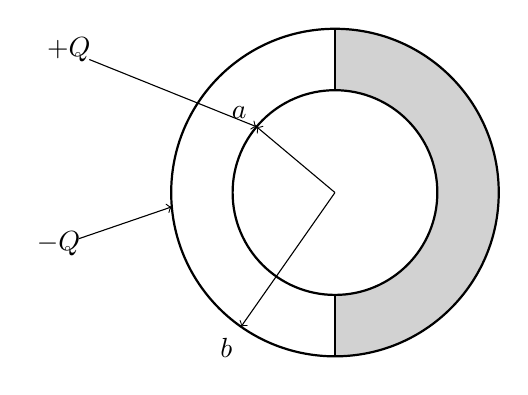
\begin{tikzpicture}[scale=1.3]
  % dielectric: right half of the annulus between r=a and r=b
  \fill[gray!35] (0,1.0) arc (90:-90:1.0) -- (0,-1.6) arc (-90:90:1.6) -- cycle;
  % spheres
  \draw[thick] (0,0) circle (1.0);
  \draw[thick] (0,0) circle (1.6);
  % interface line of dielectric halves
  \draw[thin] (0,1.0) -- (0,1.6);
  \draw[thin] (0,-1.0) -- (0,-1.6);
  % radii arrows a and b
  \draw[->] (0,0) -- (140:1.0);
  \node at (140:1.22) {$a$};
  \draw[->] (0,0) -- (235:1.6);
  \node at (235:1.85) {$b$};
  % +Q and -Q labels with arrows
  \node at (-2.6,1.4) {$+Q$};
  % Source p.172: +Q points to the inner conductor.
  \draw[->] (-2.4,1.3) -- (140:1.0);
  \node at (-2.7,-0.5) {$-Q$};
  \draw[->] (-2.5,-0.45) -- (185:1.6);
\end{tikzpicture}
\par\vspace{0.5em}\textbf{Problem 4.10}
\end{center}

\begin{enumerate}
\item[(a)] Find the electric field everywhere between the spheres.
\item[(b)] Calculate the surface-charge distribution on the inner sphere.
\item[(c)] Calculate the polarization-charge density induced on the surface of the dielectric at $r=a$.
\end{enumerate}
\solution

\textbf{(a)} Let the inner conductor carry $+Q$ and the outer one
$-Q$, as in the textbook figure. Seek a radial field
$\mathbf E=K\hat{\mathbf r}/r^2$. Its potential between the conductors,
with the outer one set to zero, is
\[
\Phi(r)=K\left(\frac1r-\frac1b\right).
\]
Both spherical conductors are equipotentials. On the plane separating
the two hemispheres, this radial field is tangential, so $E_t$ is
continuous and $D_n=0$ on both sides. Thus all interface conditions
are satisfied. A Gaussian sphere of radius $a<r<b$ gives
\[
Q=\oint\mathbf D\cdot d\mathbf a
=\epsilon_0\frac K{r^2}(2\pi r^2)
+\epsilon\frac K{r^2}(2\pi r^2)
=2\pi(\epsilon+\epsilon_0)K.
\]
Consequently, by uniqueness for positive permittivities,
\[
\boxed{\mathbf E(r)=\frac{Q}{2\pi(\epsilon+\epsilon_0)r^2}\hat{\mathbf r},
\qquad a<r<b.}
\]
For $\epsilon=\epsilon_0$ this reduces to the usual spherical-capacitor
field $Q/(4\pi\epsilon_0r^2)$.

\textbf{(b)} The free surface charge on the inner conductor is
$\sigma_f=D_r(a^+)$, since the field inside it is zero. Hence
\[
\boxed{\sigma_f=\begin{cases}
\displaystyle\frac{\epsilon Q}{2\pi(\epsilon+\epsilon_0)a^2},
&\text{hemisphere touching dielectric},\\[5pt]
\displaystyle\frac{\epsilon_0 Q}{2\pi(\epsilon+\epsilon_0)a^2},
&\text{hemisphere touching vacuum}.
\end{cases}}
\]
The two hemispheres carry $Q\epsilon/(\epsilon+\epsilon_0)$ and
$Q\epsilon_0/(\epsilon+\epsilon_0)$, respectively, which sum to $Q$.
The finite jump at the equator does not require an additional line
charge in this solution.

\textbf{(c)} In the dielectric
$\mathbf P=(\epsilon-\epsilon_0)\mathbf E$. Its outward unit normal
at its inner surface is $-\hat{\mathbf r}$, so
\[
\boxed{\sigma_{\rm pol}(a)=\mathbf P\cdot(-\hat{\mathbf r})
=-\frac{(\epsilon-\epsilon_0)Q}
{2\pi(\epsilon+\epsilon_0)a^2}.}
\]
This applies only on the dielectric hemisphere. As checks,
$\rho_{\rm pol}=-\nabla\cdot\mathbf P=0$ within the dielectric,
the flat interface has no polarization charge because $\mathbf P$
is tangential, and the bound charge at $r=b$ has opposite total
charge to that at $r=a$.

\Needspace{5\baselineskip}
\par\bigskip
\noindent\textbf{4.11}\quad The following data on the variation of dielectric constant with pressure are taken from the \emph{Smithsonian Physical Tables}, 9th ed., p.~424:

\begin{center}
\begin{tabular}{c@{\hspace{4em}}c@{\hspace{4em}}l}
\multicolumn{3}{c}{\textbf{Air at 292 K}}\\[2pt]
\toprule
\textbf{Pressure (atm)} & $\boldsymbol{\epsilon/\epsilon_{0}}$ &\\
\midrule
20 & 1.0108 & Relative density of air as a function of\\
40 & 1.0218 & pressure is given in \emph{AIP Handbook},\\
60 & 1.0333 & [3rd ed., McGraw-Hill, New York\\
80 & 1.0439 & (1972), p.~4-165].\\
100 & 1.0548 &\\
\bottomrule
\end{tabular}
\end{center}

\begin{center}
\begin{tabular}{c@{\hspace{3em}}c@{\hspace{4em}}c}
\multicolumn{3}{c}{\textbf{Pentane (C$_{5}$H$_{12}$) at 303 K}}\\[2pt]
\toprule
\textbf{Pressure (atm)} & \textbf{Density (g/cm$^{3}$)} & $\boldsymbol{\epsilon/\epsilon_{0}}$\\
\midrule
1 & 0.613 & 1.82\\
$10^{3}$ & 0.701 & 1.96\\
$4\times10^{3}$ & 0.796 & 2.12\\
$8\times10^{3}$ & 0.865 & 2.24\\
$12\times10^{3}$ & 0.907 & 2.33\\
\bottomrule
\end{tabular}
\end{center}

Test the Clausius--Mossotti relation between dielectric constants and density for air and pentane in the ranges tabulated. Does it hold exactly? Approximately? If approximately, discuss fractional variations in density and $(\epsilon/\epsilon_{0}-1)$. For pentane, compare the Clausius--Mossotti relation to the cruder relation, $(\epsilon/\epsilon_{0}-1)\propto{}$density.
\solution

Put $\kappa=\epsilon/\epsilon_0$ and
$F=(\kappa-1)/(\kappa+2)$. For fixed molecular mass and polarizability,
Clausius--Mossotti says
\[
F=\frac{N\gamma_{\rm mol}}{3}=K\rho,\qquad
\boxed{K=\frac{\kappa-1}{(\kappa+2)\rho}=\text{constant}.}
\]
It is $F$, rather than $\kappa$ or $\kappa-1$ itself, that should be
proportional to mass density.

\textbf{Air.} The pressure table alone does not specify real-gas
densities. To make the density input explicit, use the primary air
tables of Hilsenrath et al., \emph{NBS Circular 564} (1955),
Table 2-1, p.~31, for the compressibility factor
$Z_g=PV/(nRT)$.\footnote{\raggedright The source is available at
\texttt{https://nvlpubs.nist.gov/nistpubs/Legacy/circ/}\allowbreak
\texttt{nbscircular564.pdf}. The input rows, and the independent density
rows from Table 2-2, p.~37, are transcribed in
\texttt{supplementary/ch04-source/air\_reference.csv}.
This supplies a checked density source in place of the AIP reference
cited in the problem.}
The relevant rows are
\begin{center}
\begin{tabular}{rrrrr}
\toprule
$P\ (\mathrm{atm})$&10&40&70&100\\
\midrule
$Z_g(290\ \mathrm K)$&0.99623&0.98782&0.98420&0.98600\\
$Z_g(300\ \mathrm K)$&0.99717&0.99135&0.99000&0.99330\\
\bottomrule
\end{tabular}
\end{center}
Linearly interpolate in temperature,
$Z_g(292,P)=0.8Z_g(290,P)+0.2Z_g(300,P)$.
For the intervening pressures use the cubic interpolating polynomial
through the four pressure entries:
\[
Z_g(P)=\sum_{i=1}^4 Z_g(P_i)
\prod_{j\ne i}\frac{P-P_j}{P_i-P_j}.
\]
Since the temperature and composition are fixed,
$\rho\propto P/Z_g$, so the reference density cancels:
\[
\frac{\rho(P)}{\rho(20)}=\frac{PZ_g(20)}{20Z_g(P)},\qquad
\frac{K(P)}{K(20)}=
\frac{F(P)/F(20)}{\rho(P)/\rho(20)}.
\]
This gives
\begin{center}
\begin{tabular}{rrrrr}
\toprule
$P\ (\mathrm{atm})$ & $Z_g$ & $\rho/\rho(20)$ & $10^3F$ & $K/K(20)$\\
\midrule
20 & 0.99330 & 1.00000 & 3.58709 & 1.00000\\
40 & 0.98853 & 2.00965 & 7.21424 & 1.00076\\
60 & 0.98586 & 3.02264 & 10.97814 & 1.01251\\
80 & 0.98545 & 4.03185 & 14.42229 & 0.99721\\
100 & 0.98746 & 5.02955 & 17.93898 & 0.99432\\
\bottomrule
\end{tabular}
\end{center}
The ratio is approximately constant: its peak-to-peak spread is about
$1.8\%$ of its 20-atm value. Linear instead of cubic pressure
interpolation changes the normalized ratios by less than $0.05\%$,
so the percent-level conclusion does not depend on this interpolation
choice. These are approximate density-based comparisons, not a claim
of exact agreement. The dielectric data have no stated uncertainties,
so their scatter alone should not be assigned a definite microscopic
cause.

Across the range,
\[
\frac{\Delta\rho}{\rho_{20}}\simeq4.0295\quad(403.0\%),\qquad
\frac{\Delta(\kappa-1)}{\kappa_{20}-1}
=\frac{0.0548-0.0108}{0.0108}=4.0741\quad(407.4\%).
\]
Thus the density and susceptibility increase by almost the same
fraction even though each changes by roughly a factor of five.
This is expected because
$F=(\kappa-1)/[3+(\kappa-1)]\simeq(\kappa-1)/3$ for this gas.
If ideal-gas densities were used instead, $F/P$ would range from
$1.7935\times10^{-4}$ to $1.8297\times10^{-4}\ \mathrm{atm}^{-1}$,
again giving approximate agreement but omitting the real-gas correction.

\textbf{Pentane.} Here the actual densities are given. The two proposed
constant ratios are $K=F/\rho$ and the cruder
$J=(\kappa-1)/\rho$, both in $\mathrm{cm^3/g}$:
\begin{center}
\begin{tabular}{rrrrr}
\toprule
$P\ (\mathrm{atm})$ & $K$ & $K/K_1$ & $J$ & $J/J_1$\\
\midrule
1     & 0.350179 & 1.00000 & 1.337684 & 1.00000\\
1000  & 0.345826 & 0.98757 & 1.369472 & 1.02376\\
4000  & 0.341513 & 0.97525 & 1.407035 & 1.05184\\
8000  & 0.338096 & 0.96549 & 1.433526 & 1.07165\\
12000 & 0.338654 & 0.96709 & 1.466373 & 1.09620\\
\bottomrule
\end{tabular}
\end{center}
Clausius--Mossotti is again approximate: $K$ varies by about $3.45\%$
relative to its initial value, whereas $J$ rises by $9.62\%$.
It is therefore the better of the two proportionalities for these data,
but neither is exact. The endpoint fractional changes are
\[
\frac{\Delta\rho}{\rho_1}=\frac{0.907-0.613}{0.613}=0.47961,
\qquad
\frac{\Delta(\kappa-1)}{\kappa_1-1}
=\frac{1.33-0.82}{0.82}=0.62195.
\]
Density rises $47.96\%$, while susceptibility rises $62.20\%$.
The difference is consistent in direction with the local-field
correction: differentiating $F=(\kappa-1)/(\kappa+2)=K\rho$ at constant
$K$ gives
\[
\frac{d(\kappa-1)}{\kappa-1}
=\frac{\kappa+2}{3}\frac{d\rho}{\rho}.
\]
The multiplier is close to one for air, but is appreciably larger for
pentane. The tabulated residual variation of $K$ measures the remaining
failure of a strictly density-independent molecular-polarizability model.

\Needspace{5\baselineskip}
\par\bigskip
\noindent\textbf{4.12}\quad Water vapor is a polar gas whose dielectric constant exhibits an appreciable temperature dependence. The following table gives experimental data on this effect. Assuming that water vapor obeys the ideal gas law, calculate the molecular polarizability as a function of inverse temperature and plot it. From the slope of the curve, deduce a value for the permanent dipole moment of the H$_{2}$O molecule (express the dipole moment in coulomb-meters).

\begin{center}
\begin{tabular}{c@{\hspace{3em}}c@{\hspace{4em}}c}
\toprule
$\mathbf{T(K)}$ & \textbf{Pressure (cm Hg)} & $\boldsymbol{(\epsilon/\epsilon_{0}-1)\times10^{5}}$\\
\midrule
393 & 56.49 & 400.2\\
423 & 60.93 & 371.7\\
453 & 65.34 & 348.8\\
483 & 69.75 & 328.7\\
\bottomrule
\end{tabular}
\end{center}
\solution

Use Jackson's convention $\langle\mathbf p_{\rm mol}\rangle=\epsilon_0\gamma_{\rm mol}\mathbf
E_{\rm local}$, so the molecular polarizability $\gamma_{\rm mol}$ has units of
volume. Here $k$ denotes Boltzmann's constant, as in (4.81)--(4.82).
The alternative SI convention is
$\alpha=\epsilon_0\gamma_{\rm mol}$, with units $\mathrm{C\,m^2/V}$.
The ideal gas law gives $N=P/(kT)$. Applying the Clausius--Mossotti
relation (4.70) to each row, with $\delta=\epsilon/\epsilon_0-1$, yields
\[
\boxed{\gamma_{\rm mol}(T)=\frac{3kT}{P}\frac{\delta}{3+\delta},\qquad
\alpha(T)=\epsilon_0\gamma_{\rm mol}(T).}
\]
Here $P$ must be in pascals: $1\ \mathrm{cm\,Hg}=101325/76$
Pa. The resulting values are
\begin{center}
\begin{tabular}{rrrr}
\toprule
$T\ (\mathrm K)$ & $10^3/T\ (\mathrm{K}^{-1})$
& $\gamma_{\rm mol}/(10^{-28}\ \mathrm m^3)$
& $\alpha/(10^{-39}\ \mathrm{C\,m^2/V})$\\
\midrule
393 & 2.54453 & 2.87938 & 2.54946\\
423 & 2.36407 & 2.66897 & 2.36316\\
453 & 2.20751 & 2.50133 & 2.21473\\
483 & 2.07039 & 2.35455 & 2.08476\\
\bottomrule
\end{tabular}
\end{center}

For completeness, the inverse-temperature law follows by averaging the
permanent dipoles. If $p_0$ is the fixed molecular dipole magnitude and
$u$ its direction cosine with the local field, its orientation energy
is $-p_0Eu$. In a weak field $p_0E\ll kT$,
\begin{align*}
\langle p_\parallel\rangle
&=p_0\frac{\int_{-1}^1u\exp[p_0Eu/(kT)]\,du}
{\int_{-1}^1\exp[p_0Eu/(kT)]\,du}\\
&=p_0\frac{(p_0E/kT)\int_{-1}^1u^2\,du+O(E^3)}
{2+O(E^2)}
=\frac{p_0^2E}{3kT}+O(E^3).
\end{align*}
Adding a temperature-independent induced polarizability gives
\[
\gamma_{\rm mol}(T)=\gamma_i+\frac{p_0^2}{3\epsilon_0k}\frac1T.
\]
An unweighted straight-line fit $\gamma_{\rm mol}=A+B/T$ is obtained from
$x_i=1/T_i$, $y_i=\gamma_{\rm mol}(T_i)$ by
\[
B=\frac{\sum_i(x_i-\bar x)(y_i-\bar y)}{\sum_i(x_i-\bar x)^2},
\qquad A=\bar y-B\bar x.
\]
The four rows give
\[
A=6.3875\times10^{-30}\ \mathrm m^3,\qquad
B=1.10475\times10^{-25}\ \mathrm{m^3\,K}.
\]
Thus the requested dipole magnitude is
\[
\boxed{p_0=\sqrt{3\epsilon_0kB}=6.365\times10^{-30}\ \mathrm{C\,m}
\simeq6.4\times10^{-30}\ \mathrm{C\,m}.}
\]
The rounding of the data does not warrant interpreting the last digits
as an experimental precision. The largest deviation of a tabulated
polarizability from this fitted line is $0.25\%$.
\begin{center}
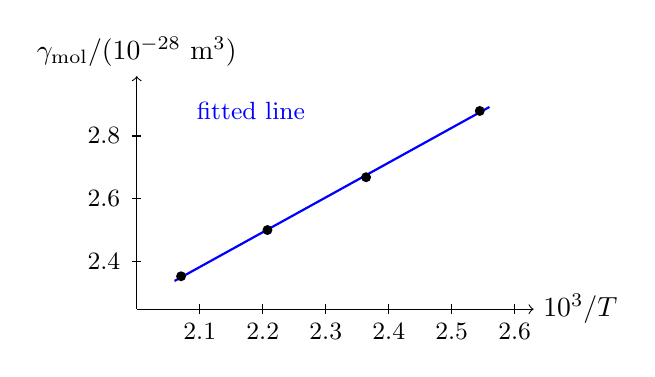
\begin{tikzpicture}[x=8cm,y=4cm]
\draw[->] (2.0,2.25)--(2.63,2.25) node[right] {$10^3/T$};
\draw[->] (2.0,2.25)--(2.0,2.99) node[above] {$\gamma_{\rm mol}/(10^{-28}\ \mathrm m^3)$};
\foreach \x in {2.1,2.2,2.3,2.4,2.5,2.6}
{\draw (\x,2.265)--(\x,2.235) node[below] {\small\x};}
\foreach \y in {2.4,2.6,2.8}
{\draw (1.993,\y)--(2.007,\y) node[left=4pt] {\small\y};}
\draw[blue,thick,domain=2.06:2.56] plot (\x,{0.0638746474+1.1047451447*\x});
\foreach \x/\y in {2.544529/2.879382,2.364066/2.668973,2.207506/2.501331,2.070393/2.354547}
{\fill (\x,\y) circle (1.8pt);}
\node[blue,anchor=west] at (2.08,2.88) {\small fitted line};
\end{tikzpicture}
\end{center}
Neglecting the small local-field correction would replace
$3\delta/(3+\delta)$ by $\delta$; retaining it as above is consistent
with the chapter's definition of molecular polarizability.

\Needspace{5\baselineskip}
\par\bigskip
\noindent\textbf{4.13}\quad Two long, coaxial, cylindrical conducting surfaces of radii $a$ and $b$ are lowered vertically into a liquid dielectric. If the liquid rises an average height $h$ between the electrodes when a potential difference $V$ is established between them, show that the susceptibility of the liquid is
\[
\chi_{e}=\frac{(b^{2}-a^{2})\rho gh\,\ln(b/a)}{\epsilon_{0}V^{2}}
\]
where $\rho$ is the density of the liquid, $g$ is the acceleration due to gravity, and the susceptibility of air is neglected.
\solution

Neglect end effects, surface tension, and changes of liquid density,
and take the external reservoir to be large enough that its level is
fixed. Write $\epsilon=\epsilon_0(1+\chi_e)$ and
$\Lambda=\ln(b/a)$. A homogeneous length $L$ of the coaxial capacitor
has radial field $E_r=V/(r\Lambda)$ and capacitance
\[
C=\frac{2\pi\epsilon L}{\Lambda}.
\]
Raising the dielectric by $dh$ replaces a length $dh$ of air, so
\[
\frac{dC}{dh}=\frac{2\pi(\epsilon-\epsilon_0)}{\Lambda}
=\frac{2\pi\epsilon_0\chi_e}{\Lambda}.
\]
At fixed voltage, the battery supplies $V\,dQ=V^2dC$, while the
field energy increases by $d(\tfrac12CV^2)=\tfrac12V^2dC$.
Their difference is available for mechanical work, hence
\[
F_{\rm electric}\,dh=\frac12V^2dC,\qquad
F_{\rm electric}=\frac{\pi\epsilon_0\chi_e V^2}{\Lambda}.
\]
Equivalently, the mechanical potential at fixed $V$ includes
$-CV^2/2$, not $+CV^2/2$.

The excess volume of liquid between the electrodes is
$\pi(b^2-a^2)h$, where $h$ is the area-averaged rise. Its weight,
after subtracting the hydrostatic support at the external free-surface
level, is
\[
F_g=\rho g\pi(b^2-a^2)h.
\]
Force balance gives
\[
\rho g\pi(b^2-a^2)h
=\frac{\pi\epsilon_0\chi_e V^2}{\ln(b/a)},\qquad
\boxed{\chi_e=\frac{(b^2-a^2)\rho gh\ln(b/a)}{\epsilon_0V^2}.}
\]
For a flat column the same result follows by minimizing
$\rho g\pi(b^2-a^2)h^2/2-C(h)V^2/2$.
The total electric force can also be checked by integrating the
leading local dielectric pressure over the annular cross section:
\[
\int_a^b\frac12(\epsilon-\epsilon_0)
\left[\frac{V}{r\ln(b/a)}\right]^2 2\pi r\,dr
=\frac{\pi\epsilon_0\chi_e V^2}{\ln(b/a)}.
\]
Thus use of the average rise is consistent with the varying radial
field. The susceptibility is positive for a liquid that rises, and
all dimensions cancel in the boxed expression.
